\documentclass{article}

% Language setting
% Replace `english' with e.g. `spanish' to change the document language
\usepackage[letterpaper,top=2cm,bottom=2cm,left=3cm,right=3cm,marginparwidth=1.75cm]{geometry}

% Useful packages
\usepackage{amsmath}
\usepackage{graphicx}
\usepackage[table]{xcolor}
\usepackage{enumerate}
\usepackage{tikz}
\usepackage{chngcntr}
\usepackage{tabularx}
\usepackage{colortbl}
\usepackage{booktabs}
\usepackage{fancyhdr}
\usepackage[a5paper,hmargin=3cm,vmargin=5cm]{geometry}
\usepackage{lscape,lipsum,graphicx}
\usepackage[absolute]{textpos}
\usepackage{fancyhdr}
\usepackage{pdflscape}
\usepackage{tocloft}
\usepackage{subcaption}
\usepackage{indentfirst}
\usepackage[colorlinks=true, allcolors=blue]{hyperref}
\usepackage{titlesec}
\titleformat{\section}{\normalfont\Large\bfseries}{}{0pt}{}

%----------------------------------Page style, header,footer--------------------------------------------
   \pagestyle{fancy}
   \fancyhf{} % clear all header and footer fields
   \fancyhead[L]{\leftmark}
   \fancyfoot[C]{\thepage}
   \renewcommand{\chaptermark}[1]{\markboth{\MakeUppercase{\chaptername\ \thechapter.\ #1}}{}}
%----------------------------------Page style, header,footer--------------------------------------------


%---------------------------------Header & Footer position when using landscape template for my page---
 \fancypagestyle{lscape}{% 
    \fancyhf{} % clear all header and footer fields 
    \fancyfoot[LE]{%
          \begin{textblock}{2}(0,5)
            \fontsize{10}{12}\selectfont{\sffamily Computer Modern}
              {\rotatebox{90}{\leftmark}}
          \end{textblock}
    }

    \fancyfoot[LO]  {%
        \begin{textblock}{1}(15,7.9)
        {\rotatebox{90}{\thepage}}\end{textblock}
        \begin{textblock}{20}(1,11.85)
        \fontsize{10}{12}\selectfont
        {\rotatebox{90}{\leftmark}}\end{textblock}
    }
    
    \renewcommand{\headrulewidth}{0pt} 
    \renewcommand{\footrulewidth}{0pt}
  }
  
  
 \fancypagestyle{firstPages}{
     \fancyhf{}
     \fancyfoot[C]{\thepage}
     \renewcommand{\headrulewidth}{0pt}
     \renewcommand{\footrulewidth}{0pt}
 }

\counterwithin{figure}{chapter}
\renewcommand{\thefigure}{\thesection.\arabic{figure}}
\counterwithout{figure}{chapter}


\begin{document}

    \vspace*{3\baselineskip}
    \pagenumbering{roman}
    \setcounter{page}{1} 
    
    \thispagestyle{firstPages}
    \begin{center}
            \begin{LARGE}
            \begin{center}
                \textf{Technical University of Crete\par}
                \newline
                \textf{School of Electrical \& Computer Engineering}
            \end{center}
        \end{LARGE}
        \vfill
        \centering
        
\includegraphics[width=0.2\textwidth]{Thesis/Figures/tucLogo.png}
        \vfill
            \begin{LARGE}
                \textf{Real time spectral classification and mapping for insitu detection of plant pathologies\par\bigskip Panagiotis Takas}
            \end{LARGE}
        \vfill
        
        \begin{center}
           \begin{Large}
             \textf{Thesis Committee\par}
             \justifying
             \textf{Costas Balas, Professor (supervisor)\par}
             \textf{Aggelos Bletsas, Professor\par}
             \textf{Basilis Samoladas, Professor\par}
           \end{Large}
        \end{center}
    
    \end{center}
    
    \newpage
        \thispagestyle{empty}
        \mbox{}
        
    \newpage
    \thispagestyle{firstPages}
    
    \begin{large}
         \begin{Large}
            \centering
            \textbf{Abstract}
         \end{Large}
         \vspace*{3\baselineskip}
         
         \justifying
         \textf{Spectroscopy is the study of interaction between matter and light to obtain structural and chemical information. Spectral imaging uses a plethora of narrow-band images across the electromagnetic spectrum to collect and analyze this kind of spectroscopic and imaging information at the same time. Spectroscopic information can be used to create chemical maps of the imaged area through capturing the spectrum of each individual pixel of the image and using it as data set for classification algorithms.For this purpose a hyperspectral camera has been acquired to collect data and detect abnormalities and pathologies in plants and then study if they are detectable from an early stage.The acquired data were classified using clustering algorithms which were developed using Qt Firmware for the GUI and C++ for the main source. In an effort to achieve real time mapping and optimal spectral classification, the usage of GPU's computational capability was mandatory .The produced maps consist of pseudocolors where each pseudocolor corresponds to a cluster of pixels with spectral similarities. These similarities along with broadly used vegetation indices were studied in plants which have been submitted under stressful conditions (e.g. increased salinity) using our developed algorithms. The findings from the experiment highlight the potential for an early detection of plant's destruction.\par}
    \end{large}
    
     \newpage
        \thispagestyle{empty}
        \mbox{}
        
    \newpage
    \thispagestyle{firstPages}
       
    \begin{large}
         \centering
         \begin{Large}
            \textbf{Acknowledgements}
         \end{Large}
         \vspace*{3\baselineskip}
         
         \raggedright
         \textf{First of all i would like to thank my family for their invaluable support through the years of my studies. I would like to thank my supervisor professor Costas Balas for his support and guidance through my thesis. He entrusted me an unknown field and the challenge broadened my mind and scientific background. I would like to thank Phd Candidate Athanasios Tsapras for the support on the experimental procedure. Special thanks goes to all my friends and people I’ve met through the years of my studies in Chania.\par}
    \end{large}
    \newpage
    \vspace*{4\baselineskip}
    
    {
        \hypersetup{linkcolor=black}
        \setlength{\parindent}{0.5cm}
        \setlength{\parskip}{1em}
        \vspace{10pt}
        \tableofcontents
        
        \renewcommand{\cftsecleader}{\cftdotfill{\cftdotsep}}
        \renewcommand{\cftsecfont}{\mdseries}
        \renewcommand{\cftsecaftersnum}{\hspace{0.5em}}
        \cftsetpnumwidth{2em}
        \cftsetrmarg{3em}

        
        \singlespacing
        \newpage
        
        \listoffigures
        \newpage
        
        \listoftables
        \newpage

        \section{Introduction}
            \pagenumbering{arabic}
            \setcounter{page}{1}
            
            \hspace{0.5cm}Light is a form of electromagnetic radiation that is visible to the human eye. The color we see is a result of which wavelengths are reflected back to our eyes and which is absorbed. Visible wavelengths are a small part within the electromagnetic spectrum. The color of visible light depends on its wavelength and can be ranged from 380nm at the violet end to 700nm at red end. Color is an important part of our everyday lives and is used to convey information, create atmosphere, and help us identify things. Color can also be used to create illusions, manipulate our perception of space, size and distance. So the question arises, what if the human eye could detect a broader range of light's spectrum by using technical means? \par
            Spectral imaging technology is the process of collecting and processing information from across the electromagnetic spectrum. It involves capturing images with different wavelengths of light, which can range from visible to near-infrared and short-wave infrared. The goal of spectral imaging is to obtain the spectrum for each pixel in the image of a scene, with the purpose of finding objects, identifying materials and monitoring changes in the environment.\par
            Hyperspectral imaging is a more advanced version of spectral imaging. It collects and processes information from a much wider portion of the electromagnetic spectrum, from visible to near-infrared,short-wave infrared and beyond. The goal of hyperspectral imaging is to obtain the spectrum of each pixel in the image of a scene, with the purpose of finding objects,identifying materials and monitor changes in the environment.Hyperspectral imaging is a technique that can be used to detect plant pathologies by analyzing the reflection of light from the plant's leaves in many narrow, contiguous wavelength bands. This allows for the identification of specific chemical compounds and structural features that are associated with different types of plant diseases. For example, a diseased plant may have a different spectral signature than a healthy plant, due to changes in chlorophyll content or the presence of pigments produced by the pathogen. By analyzing these spectral signatures, it is possible to identify and map the extent of diseases in a field or greenhouse, even before visible symptoms appear.\par
            The key advantage of hyperspectral imaging over traditional methods of plant pathology detection is that it can provide detailed information about the health of the entire plant, rather than just a small sample. This allows for early detection and rapid response to outbreaks of disease, which can help to minimize crop losses. The technology is considered as powerful tool that could be used by farmers, agronomist, researcher, and agtech company.\par
            Spectroscopy can be used to detect early stages of plant pathologies in plants. This technique is non-invasive, non-destructive and cost-effective, allowing for accurate diagnoses without the need for sample preparation. Spectral data can be used to discern differences in plant chemistry, physiology, and health, with certain wavelengths providing insight into the presence of disease. \par
            Hyperspectral imaging is an advanced approach which uses artificial intelligence to detect plant diseases. By utilizing spectroscopy to detect plant pathologies, early stages of diseases can be identified and eradicated, mitigating their effects and preventing further spread.\par
            Insitu detection of plant pathologies refers to the identification of diseases in plants while they are still in the field,rather than bringing samples back to a laboratory for analysis. This can be useful for quickly identifying and addressing diseases in crops, which can help to reduce losses and improve crop yields. There are a few different approaches that can be used for insitu detection of plant pathologies, including visual inspection,use of portable diagnostic tools, and remote sensing techniques. Visual inspection involves simply looking for signs of disease on the plants, such as discoloration, wilting, or abnormal growth patterns. Portable diagnostic tools, such as handheld spectrometers, can be used to analyze the chemical composition of plants and identify any abnormalities that might be indicative of disease.Remote sensing techniques, such as satellite imagery or drone-based imaging, are being used to detect plant diseases from a distance.\par
            \newpage
            
            \subsection{Experiment}
                    \hspace{0.5cm}The purpose of this experiment was to investigate the potential identification of plant growth abnormalities using spectroscopy. Two groups of tomato plants were grown, with one group exposed to stressful conditions. Spectroscopic analysis was performed
                    on the plants at various stages of growth to detect any potential signs of plant pathology. The results of this experiment have the potential to provide valuable insights into the effects of stressful conditions on plant growth and health, as well as aid in the early detection of plant pathogens. The spectroscopic analysis used in the study is non-destructive and non-invasive, making it an ideal method for monitoring plant health. Overall, this study highlights the importance of understanding the impact of environmental factors on plant growth and health, and the potential benefits of using spectroscopy as a tool for early detection of plant pathology.\par 
                    A key aspect of this research was the classification method used to analyze the spectroscopic data. We compared classification algorithms based on results and execution time then we employed an unsupervised learning technique, specifically a K-means clustering algorithm, which has been widely used in the literature for vegetation classification and will be further discussed in the next chapters. This method allowed us to accurately classify the plants with the purpose of finding any abnormalities.\par 
                    Another important aspect of this research was the use of vegetation indices, which are mathematical transformations of the original spectral data. These indices can provide additional information about the plants, such as their chlorophyll content or water stress, that is not directly observable from the raw spectra. We used several commonly used vegetation indices, such as the Normalized Difference Vegetation Index (NDVI) and the Enhanced Vegetation Index (EVI), which have been shown to be effective in vegetation studies. Nevertheless more indices where used and analyzed in order to reach our own conclusions about their use.\par 
                    Finally, we also analyzed the practicality of different spectral bands for vegetation analysis. We measured the reflectance of light at different wavelengths, and different plant characteristics can be related to specific spectral bands. Our analysis showed that the red and near-infrared bands are particularly useful for vegetation analysis, as they can provide information about the green vegetation and the chlorophyll content of the plants.\par 
                    In conclusion, this thesis demonstrated the importance of using an appropriate classification method, vegetation indices and spectral bands for vegetation spectroscopy studies. Spectral bands that we used were key elements to obtain accurate results, and the use of these methodologies can be applied in future studies to understand the effects of environmental factors on plant growth and health, and the potential benefits of using spectroscopy as a tool for early detection of plant pathology.
                    \newpage
            
            \vspace*{1\baselineskip}
            \textbf{Chapter 2: Hyperspectral Imaging & Classification}\par
            In this chapter, we delve into the fundamentals of hyperspectral imaging, a powerful tool for analyzing materials and extracting valuable information from images. We begin by discussing the physics behind the technology and how it differs from traditional imaging methods. Next, we explore the various techniques used in hyperspectral imaging, including classification and K-means clustering. We also examine the different initialization methods and similarity measures used in K-means clustering.\par
            \textbf{Chapter 3: Pathologies in Plants & Vegetation Indices}\par
            This chapter focuses on the impact of light on plant growth and how pathologies can manifest in plants. We first examine the visible effects of plant pathologies and how they can be detected and diagnosed. We also explore the use of vegetation indices in the crop industry and how they can be used to assess plant health. We discuss the effects of salinity in plants and how vegetation indices can be used to monitor these effects. Additionally, we delve into remote sensing in plants, including advancements in spectral imaging for food quality control and vegetation identification.\par
            \textbf{Chapter 4: Experiment & Research}\par
            This chapter details the experimental methods used in our study. We describe the hyperspectral imaging system used and how it was calibrated. We also discuss the software and algorithm development necessary for analyzing the data.\par
            \textbf{Chapter 5: Results & Conclusions}\par
            In this final chapter, we present the data collected from our experiments and discuss the results. We first examine the pathologies observed and the vegetation indices used to assess plant health. We then provide clarification on the data presented in tables. Finally, we summarize our findings and draw conclusions on the effectiveness of hyperspectral imaging and vegetation indices in monitoring plant health.\par
            
            \newpage
        \section{Hyperspectral Imaging and Classification}
            \setcounter{figure}{0}
            \subsection{Physics}
                \hspace{0.5cm}Light is a form of electromagnetic radiation, which is a type of energy that travels through space in the form of waves. Electromagnetic radiation includes radio waves, microwaves, infrared radiation, visible light, ultraviolet radiation, X-rays, and gamma rays. Each type of electromagnetic radiation has a different wavlength and frequency. The electromagnetic spectrum is the range of all types of electromagnetic radiation.\par
                Max Planck, a German physicist, formulated an equation that describes the relationship between the energy of the electromagnetic wave and its frequency. This equation, known as Planck’s Law, forms the basis of our understanding of the relationship between electromagnetic radiation and energy.\par
                \begin{align*}
                    E &= hf && \text{(2.1)} \\
                    \text{and since } f &= \frac{c}{\lambda} && \text{(2.2)} \\
                    E &= \frac{hc}{\lambda} && \text{(2.3)}
                \end{align*}
                
                \noindent
                \hspace{0.5em}Where:
                \begin{enumerate}
                    \setlength\itemindent{1.5em}
                    \setlength\leftskip{0.5em}
                    \item $E$ defines the energy of the electromagnetic wave (photon energy).
                    \item $h$ is Planck's constant and defines the relationship between the energy of a photon and its frequency.
                    \item $f$ is the frequency of the electromagnetic wave.
                    \item $c$ is the velocity of light.
                    \item $\lambda$ defines the wavelength of the electromagnetic wave.
                \end{enumerate}
                
                The electromagnetic spectrum is a continuum of all electromagnetic waves arranged according to frequency and wavelength. The visible portion of the electromagnetic spectrum is the portion that the human eye can detect. This range is between 380 and 700 nanometers. As it is shown in figure 2.1 electromagnetic spectrum has been segmented. These segmentations refer to different energy contents which are applied in different applications.\par
                
                \begin{figure}[htb]
                    \centering
                    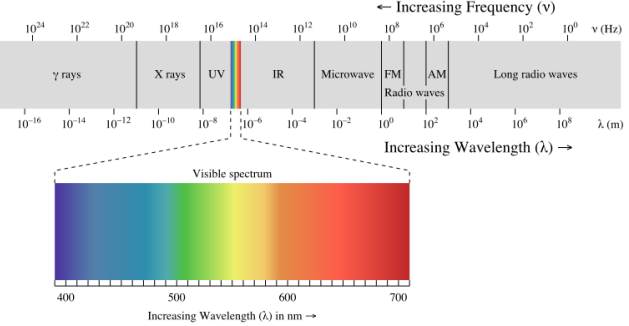
\includegraphics[width=0.9\textwidth]{Figures/electromagneticSpectrum.PNG}
                    \caption{Electromagnetic Spectrum}
                    \label{fig:example}
                \end{figure}
                
                When light travels through space without interacting with an obstacle its energy remains the same. However when light travels through different objects five interactions can take place : Emission,Absorption,Transmission,Scattering and Luminescence. Each phenomena of light depends on its wavelength and the characteristics of the material it interacts with. The material type also determines the type of interaction that will take place. Some materials are better at transmitting light, while others are better at reflecting light. The amount of light that gets absorbed or reflected also depends on the nature of the material and its surface. For example, a rough surface will tend to scatter or diffuse light, while a smooth surface will tend to reflect or transmit light.\par
                \vspace*{1\baselineskip}
                
                \textbf{Emission}
                \vspace*{1\baselineskip}
                
                \hspace{0.5cm}Emission is the process through which a material releases energy as radiation. In this process, the material absorbs energy from its surroundings, which causes the electrons in its atoms to become excited. When the excited electrons return to their original energy state, the energy is released in the form of photons, which is a form of electromagnetic radiation. The wavelength of the emitted radiation is determined by the energy of the electrons, with higher energy resulting in shorter wavelengths and lower energy resulting in longer wavelengths. The energy of the photons emitted by a material is also determined by the material’s temperature, with hotter materials emitting more energy than colder materials.\par
                \vspace*{1\baselineskip}
                
                \textbf{Absorption}
                \vspace*{1\baselineskip}
                
                \hspace{0.5cm}Light absorption is the process in which light is absorbed by matter and converted into energy. In an atom, electrons vibrate at a specific frequency – this is called the natural frequency. If a wave of light hits a material in which the electrons are vibrating at the same frequency as the wave of light, the electrons will absorb the energy and convert it into vibrational motion. This is why objects have different colours – different materials’ electrons will vibrate at different rates, and therefore absorb different frequencies of light. The amount of energy that an electron needs to ”jump” from one energy level to another equals the energy gap between those levels. This energy can be acquired through means of radiation,heat etc. and this phenomena is called absorption.Atoms however have the tendency to remain in low energy levels. So after a while the electron returns back to ground state releasing energy equal to the energy gap.To further understand what is absorption and emission graphical examples are presented.\par  
                
                \begin{figure}[htb]
                    \centering
                    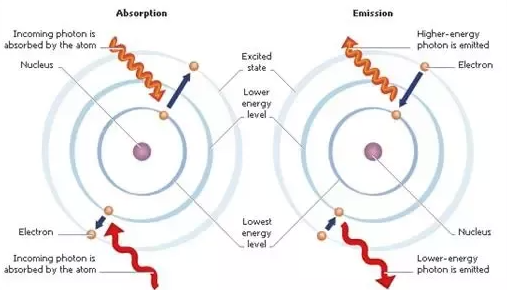
\includegraphics[width=0.9\textwidth]{Figures/atmAbsEm.PNG}
                    \caption{ Absorption - Emission}
                    \label{fig:example}
                \end{figure}
                
                \begin{figure}[htb]
                    \centering
                    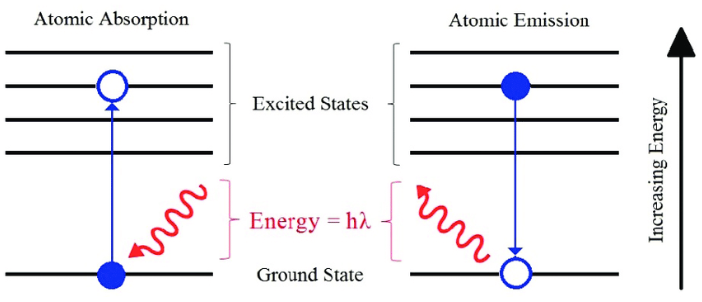
\includegraphics[width=0.9\textwidth]{Figures/AbsorbEm.PNG}
                    \caption{ Absorption - Emission}
                    \label{fig:example}
                \end{figure}
                \newpage
                
                \textbf{Transmission}
                \vspace*{1\baselineskip}
                
                \hspace{0.5cm}Transmission is the process where electromagnetic radiation passes through a material without getting absorbed. In this process, the material acts as a medium through which the radiation can travel and it does not absorb the radiation. The material does not become excited when the radiation passes through it, which means that it stays unchanged and without any energy loss.\par
                \vspace*{1\baselineskip}
                
                \textbf{Scattering}
                \vspace*{1\baselineskip}
                
                \hspace{0.5cm}Scattering of light is the process by which light is reflected in all directions when it interacts with matter. This phenomenon is caused by the individual particles of matter reflecting the light in different directions. This is why we can see objects even when they are not directly illuminated by a light source. For example, when sunlight hits a cloud, it is scattered and reflected in different directions, giving us an illuminated sky even when the sun is not directly visible. There are three main different types of light scattering and are generally differentiated based on the size of the particles relative to the wavelength of light and the presence or absence of a surrounding medium : 1.Rayleigh Scattering: It occurs when light scatters off particles that are much smaller than the wavelength of light leading to weak, uniform scattering in all directions. The color of the scattered light is blue, as seen in the blue of the sky. 2.Mie Scattering: It occurs when light scatters off particles that are larger than the wavelength of light resulting in more intense and directional scattering. Mie scattering is usually seen in clouds, where light scatters off water droplets. 3.Tyndall Scattering: It occurs when light scatters off particles in a colloidal suspension, such as a solution of particles in a liquid.In Tyndall scattering, the particles are still larger than the wavelength of light, but they are suspended in a medium, leading to light scattering that is confined to a specific direction. Tyndall scattering is responsible for the light blue color seen in a glass of milk.\par
                \vspace*{1\baselineskip}
                
                \textbf{Luminescence}
                \vspace*{1\baselineskip}
                
                \hspace{0.5cm}Luminescence is the emission of light produced by means other than heat.Luminescence is caused by the movement of electrons into different energetic states. There are many different types of luminescence including bioluminescence, chemiluminescence, phosphorescence, and fluorescence. Fluorescence and phosphorescence occur when light is emitted by an object exposed to electromagnetic radiation. The main factor that distinguishes fluorescence from phosphorescence is the duration of light emission. In fluorescence, the light emission is short-lived and stops as soon as the excitation light is turned off. The process is usually completed within a few nanoseconds to microseconds. In contrast, phosphorescence is characterized by a longer duration of light emission, often continuing for several milliseconds to seconds after the excitation light is turned off. Another factor that distinguishes the two is the mechanism of light emission. Fluorescence occurs due to a rapid transition of an excited electron from a higher energy state to a lower energy state, while phosphorescence occurs due to a slower transition of an excited electron from a higher energy state to a lower energy state.
                \vspace*{5\baselineskip}
                
                \begin{figure}[htb]
                    \centering
                    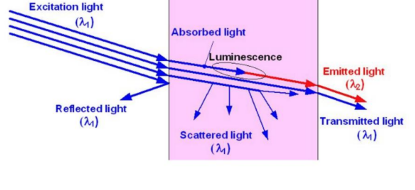
\includegraphics[width=0.8\textwidth]{Figures/lightPhen.PNG}
                    \caption{Light interactions}
                    \label{fig:example}
                \end{figure}
            \newpage
            \subsection{Hyperspectral Imaging}
                \hspace{0.5cm}Hyperspectral imaging (HSI) is a technique that analyzes a wide spectrum of light instead of just assigning primary colors (red, green, blue) to each pixel. The light striking each pixel is broken down into many different spectral bands in order to provide more information on what is imaged.HSI is related to spectroscopy, which is the study of how matter interacts with light to produce a spectrum. Spectroscopy provides a way to identify materials based on their unique spectral signatures and hyperspectral imaging produce two-dimensional images that can be used for mapping, monitoring, and analysis. This results in a ”spectral signature” for each pixel in an image, which can be used to identify specific materials or substances.\par
                A hyperspectral cube can be thought of as a stack of images, one on top of the other, where each image in the stack represents the field of view (FOV) at a particular wavelength-band of light.Thus a two-dimensional image in view is represented by a three-dimensional image-cube where the third dimension represents optical wavelength.\par
                \vspace*{2\baselineskip}
                
                \begin{figure}[htb]
                    \centering
                    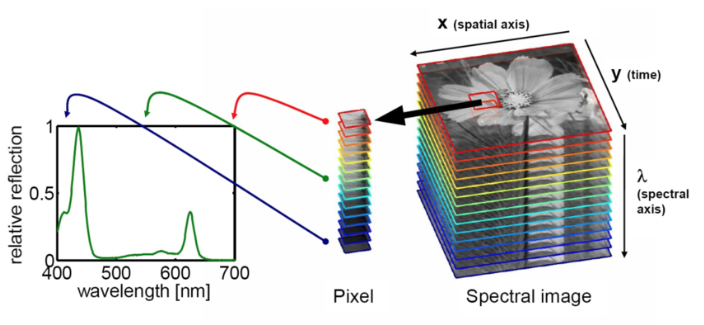
\includegraphics[width=0.72\textwidth]{Figures/HyperspectralCube.PNG}
                    \caption{Hyperspectral Cube}
                    \label{fig:example}
                \end{figure}
                
                An HSI system consist of an imaging sensor,band-pass filters to allow particular segments of the spectrum to pass in, a light source and a computer to process the data and perform the analysis. This data are images acquired from a steady sample targeted by different wavelengths of light (hyperspectral cube). Each pixel of the images contains information about the spectrum of any object and can be either continues or discrete.\par
                The molecular structure of an object determines how it interacts with light because it determines which wavelengths of light are absorbed, transmitted, or reflected by the object. When light interacts with a molecule, it can be absorbed, causing the electrons in the molecule to become excited and move to higher energy levels. The energy of the absorbed light depends on the wavelength, and different molecules absorb different wavelengths of light based on their molecular structure. This absorption can cause the molecule to vibrate or rotate, which can in turn cause the molecule to emit radiation. The reflected and transmitted light also depend on the molecular structure, as the arrangement of atoms and bonds in a molecule can affect how light is scattered or refracted as it passes through or bounces off the object.\par
                \vspace*{2\baselineskip}
                
                \begin{figure}[htb]
                    \centering
                    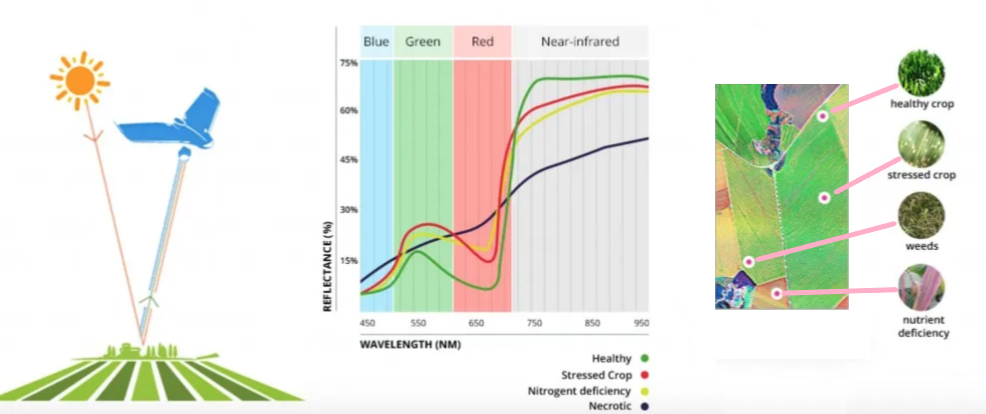
\includegraphics[width=0.75\textwidth]{Figures/spectrumPlant.PNG}
                    \caption{Example of spectrum used in crop industry}
                    \label{fig:example}
                \end{figure}
                
                \vspace*{2\baselineskip}
                
                \begin{figure}[htb]
                    \centering
                    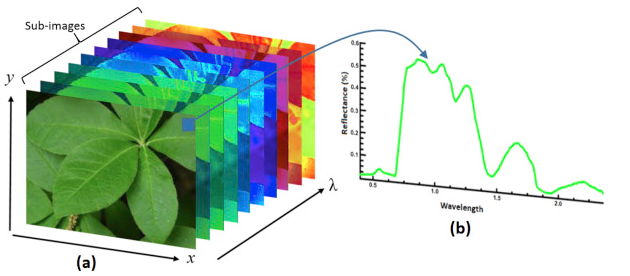
\includegraphics[width=0.72\textwidth]{Figures/pixelCube.PNG}
                    \caption{ A spectral image is a three dimensional data cube with two spatial dimensions (x and y) and one spectral dimension (\λ) resembling the reflection spectrum at every pixel}
                    \label{fig:example}
                \end{figure}
                
                Hyperspectral imaging and classification are closely related, as hyperspectral imaging is a powerful tool for acquiring high-dimensional data, while classification is the process of analyzing this data to identify specific objects or patterns. Hyperspectral imaging collects information across a range of electromagnetic wavelengths, generating a spectrum for each pixel in the image. This provides a wealth of information that can be used to distinguish between different materials, such as crops or minerals, based on their unique spectral signatures. Classification algorithms are then applied to this data to identify and label specific features, such as different crop types, water sources, or land cover types. These algorithms can be trained using various machine learning techniques, to accurately classify the data. In many fields, including agriculture, hyperspectral imaging and classification are used to enable more precise and accurate analysis of complex data sets. The result and the proximity of the classification is inextricably linked with the hsi system used that acquired the data.\par
                There are several steps involved when using a hyperspectral imaging system to acquire and analyze data. The following are the general steps that are typically followed in a hyperspectral imaging process:\par
                 \begin{enumerate}
                 \item Design the Experiment: The first step is to define the research question or objective and design the experiment to achieve that objective. This includes selecting the hyperspectral imaging system, determining the sampling strategy, and identifying the specific parameters to be measured.
                 \item Data Acquisition: The next step is to acquire the hyperspectral data by scanning the target area or object. The hyperspectral imaging system captures data across a range of electromagnetic wavelengths, generating a spectrum for each pixel in the image.
                 \item Data Preprocessing: The acquired data is preprocessed to reduce noise, correct for distortion, and normalize the data to remove any variations in the illumination or reflectance. This step ensures that the data is suitable for further analysis.
                 \item Data Analysis: The preprocessed data is analyzed using various techniques, including machine learning. This step involves identifying patterns and relationships in the data that can be used to extract useful information.
                 \item Interpretation: The final step is to interpret the results and draw conclusions based on the analyzed data. This step involves using domain-specific knowledge to  interpret the patterns and relationships identified in the data and relate them to the research question or objective. It is achieved usually using pseudo maps.
                 \end{enumerate}
                 These steps may vary depending on the specific application of the hyperspectral imaging system, but they generally reflect the general process of acquiring and analyzing hyperspectral data.
                 \newpage
                 
            \subsection{Classification}
                    \hspace{0.5cm}Classification is the process of assigning objects or data to predefined categories or classes based on their attributes. This task is commonly performed in the field of pattern recognition, where meaningful patterns are identified in data, relevant features are extracted, and those features are used to classify new data. This process allows for the automatic assignment of new objects or data to their respective classes based on similarities or differences with existing data. There are two types of classification algorithms: supervised and unsupervised.\par
                
                \textbf{Supervised Classification}
                
                    \hspace{0.5cm}Supervised classification involves training a computer algorithm on labeled data, which is divided into a training set and a testing set. The labeled training set is used to train the model to recognize patterns in the data, and the model is then applied to the testing set to evaluate its accuracy. The goal of supervised classification is to identify predetermined classes or categories in the data. This approach is useful when the desired output is known in advance, as the labeled data provides a clear indication of what the model should be looking for. In various industries, classification algorithms are used to identify entities by utilizing a database containing information on their spectral signature.\par
                
                \textbf{Unsupervised Classification}
                
                    \hspace{0.5cm}Unsupervised classification is where the outcomes (groupings of pixels with common characteristics in this case) are based on the software analysis of an image without using previous knowledge of label data. The computer uses techniques to determine which pixels are related and groups them into classes. The user can specify which algorithms the software will use and the desired number of output classes. Unlike supervised classification, unsupervised classification does not require preexisting labels or categories to be assigned to the data. This approach is used when the desired output is not known or when labeled data is not available. Unsupervised classification can identify hidden structures and relationships in the data, such as clusters or groups of data points that are similar to each other. The goal of unsupervised classification is to explore and discover patterns in the data that may not be immediately visible. Unsupervised classification is a useful technique for exploratory data analysis and can help to reveal patterns that can be used to generate hypotheses for further investigation.\cite{Alpaydin E.}
                    
                    Overall, classification is a crucial task in pattern recognition that allows for the automatic assignment of new data to predefined categories or classes based on their attributes. Both supervised and unsupervised classification have their own advantages and disadvantages, and their use depends on the specific task and available data.
                    
                    \begin{figure}[h]
                        \centering
                        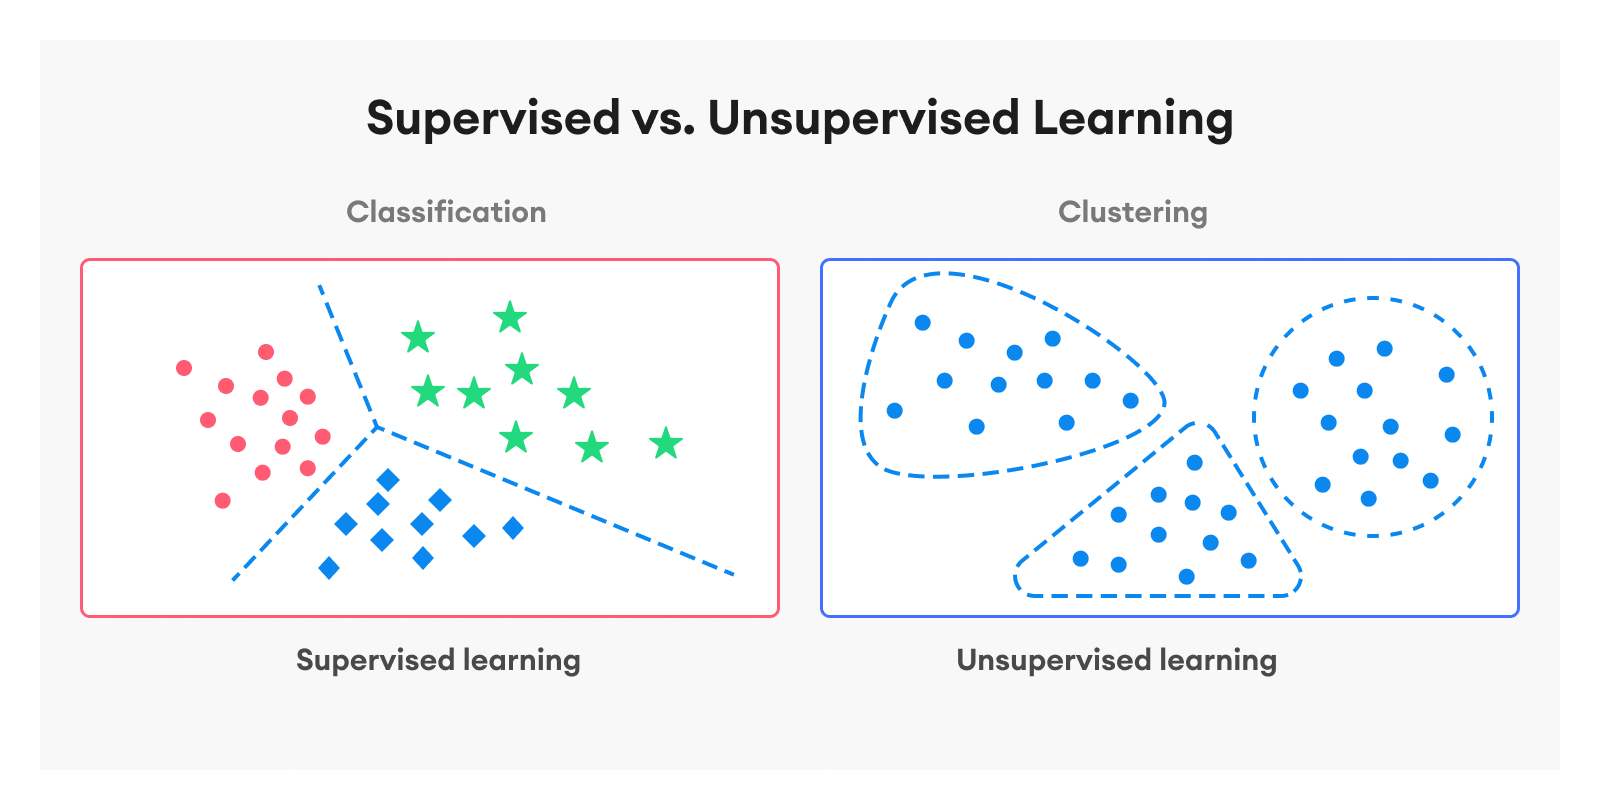
\includegraphics[width=0.8\textwidth]{Figures/supUnsup.png}
                        \caption{Supervised \& unsupervised learning}
                        \label{fig:my_label}
                    \end{figure}
                    \newpage
                    \subsection{K-Means}
                    
                    \hspace{0.5cm}K-means classification is used for a variety of purposes, such as crop yield estimation, crop disease detection, and soil analysis. It is broadly used to group satellite imagery of crop fields into clusters based on crop type, soil type, or plant health. By grouping similar data points together, farmers can better understand the spatial variability within their fields and make more informed decisions about planting, fertilizing, and harvesting. K-means can also be used to analyze soil data, such as nutrient content and texture, to identify areas of the field that may require more or less fertilizer etc. . Overall, it is a powerful tool for uncovering patterns and structure in industries and can help make more efficient and sustainable decisions.\par
                    The k-means algorithm involves 3 steps, starting with the selection of k number of clusters. The algorithm then randomly selects k number of data points to serve as initial centroids. The remaining data points are then assigned to the nearest centroid based on their similarity. The centroids are then updated based on the mean of the data points in each cluster. This process is repeated until the centroids no longer change or a maximum number of iterations is reached. The final result is a set of k clusters, with each data point-pixel assigned to one of them. \par

                    \begin{enumerate}
                        \item Centroid Initialization
                        \item Assigning data points to clusters
                        \item Updating Centroids
                    \end{enumerate}
                    
                    \textbf{Step 1: Centroid Initialization}
                    The first step of the K-Means algorithm is to randomly initialize the centroids for each cluster. The number of centroids is equal to the number of clusters that we want to create. Typically, the centroids are initialized by randomly selecting k data points from the dataset, where k is the number of clusters.\par

                    \textbf{Step 2: Assigning Data Points to Clusters}
                    In the second step, each data point in the dataset is assigned to its nearest centroid. The distance between each data point and the centroids is calculated using a distance metric, such as Euclidean distance. Each data point is assigned to the cluster whose centroid is closest to it. This step creates the initial set of clusters.\par

                    \textbf{Step 3: Updating Centroids}
                    In the third step, the centroids for each cluster are updated. The updated centroid is the mean of all the data points assigned to that cluster. Specifically, the centroid is calculated by taking the average of the values of all the data points assigned to the cluster along each dimension. This step results in a new set of centroids. The second and third steps are repeated iteratively until convergence, meaning the centroids no longer move or the maximum number of iterations is reached.\par
                    
                    \textbf{Centroid:} A table that contains representative values of each cluster - each cell of the table represents a channel (an image of the cube).

                    \textbf{Cluster:}   A group of data with common characteristics.
                    
                    The term nearest centroid is defined by a similarity measure which refers to the metric used to determine how similar or dissimilar two data points are to each other based on an equation. Euclidean, Cosine,Spectral Angle Mapper (SAM) and more similarity measures were compared in order to determine apart from their prerformance,their execution time too since it is also a key factor to help improve the speed and efficiency for in situ analysis and detection of plant pathologies.\par
                    Performance of various classification algorithms was evaluated using a calibration tool designed for use in the digital imaging industry, Macbeth Training Cube MONO.The Macbeth Training Cube MONO is a calibration tool designed for use in the digital imaging industry. It is essentially a color calibration chart that is used to ensure that the colors captured by a digital camera or other imaging device are accurate and consistent. The chart consists of a series of colored squares arranged in a specific pattern, with each square representing a different color. By photographing the chart under controlled lighting conditions, the color values captured by the camera can be compared to the known color values of the chart, allowing for accurate color correction and calibration. It has a total number of 140 patches and 96 unique colors among those patches. The evaluation of the performance was executed in the subsequent manner:
                    
                    \begin{enumerate}
                        \item Classification algorithm (k-means) was executed on the exact same sample (data) using various similarity measures.
                        \item The number of clusters assigned only to patches with unique colors was calculated in proportion to the total number of clusters assigned.
                        \item The resulting two numbers were divided, and the quotient represented the percentage of algorithm performance.
                    \end{enumerate}
                    
                    \vspace*{2\baselineskip}
                    \begin{figure}[h]
                        \centering
                        \subfloat{{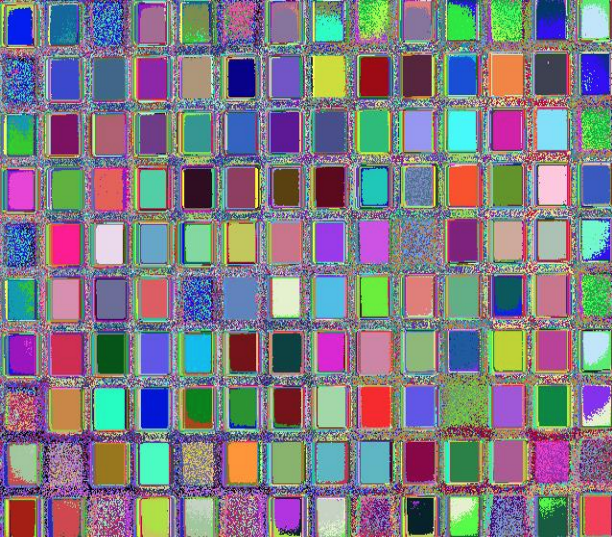
\includegraphics[width=6.5cm,height=4cm]{Figures/MacBethClassed.PNG} }}
                        \qquad
                        \subfloat{{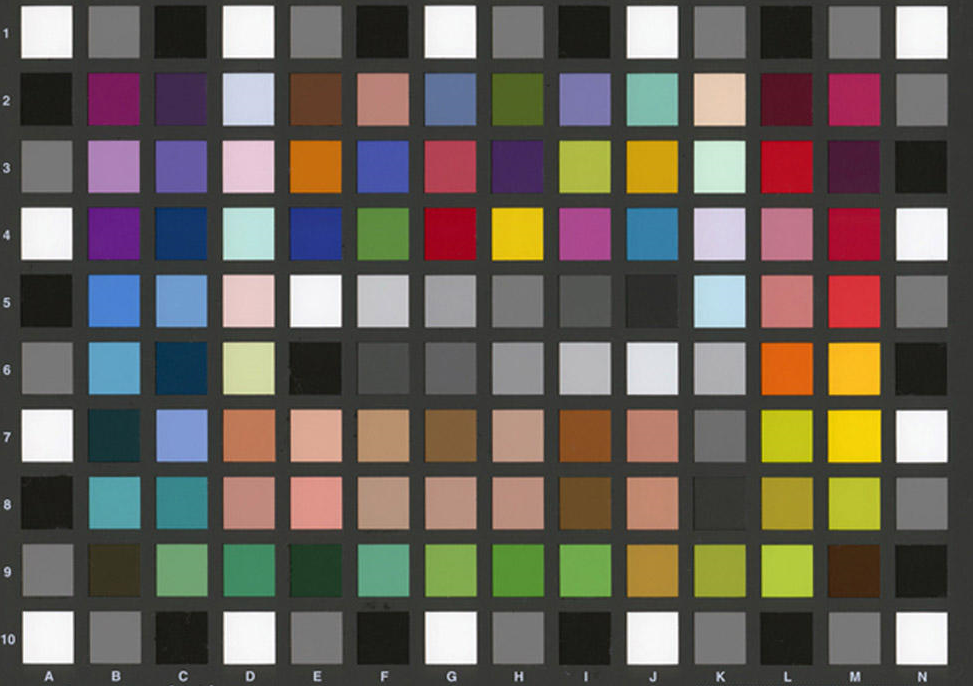
\includegraphics[width=6.5cm,height=4cm]{Figures/macbeth.png} }}
                        \caption{K-Means used on Macbeth Colorchecker (right image) during performance evaluation producing a pseudo-color map (left image)}%
                        \label{fig:example}
                    \end{figure}
                    \vspace*{4\baselineskip}
                    
                    \begin{figure}[h]
                        \centering
                        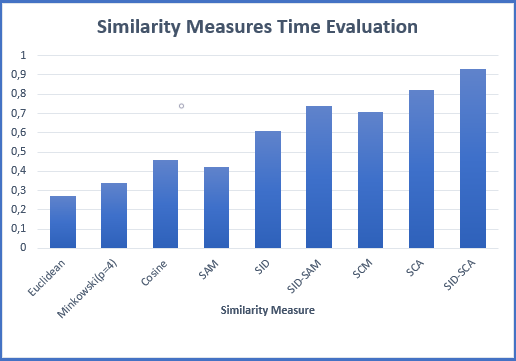
\includegraphics[width=0.75\textwidth]{Figures/ExTime.PNG}
                        \caption{Execution time per iteration for some widely used similarity measures}
                        \label{fig:example}
                    \end{figure}
                
                    \begin{figure}[h]
                        \centering
                        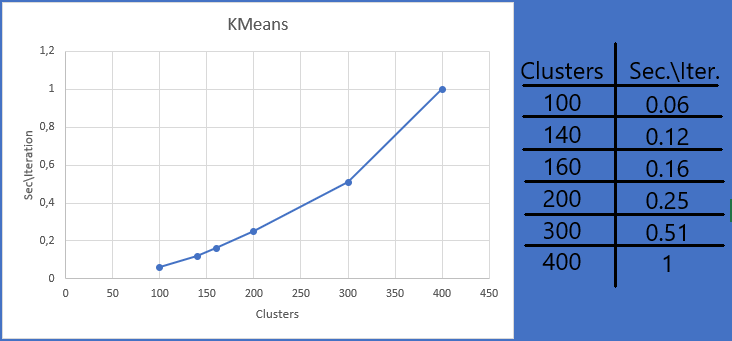
\includegraphics[width=0.75\textwidth]{Figures/KmeansTime.PNG}
                        \caption{Execution time per iteration in regards to the number of clusters}
                        \label{fig:example}
                    \end{figure}
                    \vspace*{10\baselineskip}
                    \newpage
                
                \subsubsection{Initialization Methods}
                \hspace*{0.5cm}Initialization methods in KMeans determine the initial position of the centroid's value that represent the clusters. The choice of initialization method can greatly affect the performance, accuracy and execution time of the algorithm. There are several initialization methods used, and each has its own advantages and disadvantages. Determing the suitable for the application initialization method can save valuable compuational resources,time and unnecessary algorithm iterations.\par
                One of the most commonly used initialization methods is the random initialization method. In this method, the initial centroids are randomly selected from the data points. This approach is simple and easy to implement, but it can result in suboptimal clustering results, as the initial centroids may not be representative of the data distribution. Its key advantage its the zero time consumption.\par
                To address this issue, a more sophisticated initialization method called Kmeans++ was proposed. Kmeans++ works by iteratively selecting the initial centroids based on the distance from the previously selected centroids. This approach ensures that the initial centroids are well-distributed and representative of the data distribution, leading to improved clustering performance.\par
                The farthest point initialization method, also known as the furthest-first traversal method, works by selecting the initial centroids as the data points that are farthest away from each other. This approach ensures that the initial centroids are well-distributed and can provide a good initial estimate of the data distribution. However, this method is computationally expensive, especially when dealing with high-dimensional data.\par
                While both Kmeans++ and the farthest point initialization method aim to choose initial centroids that are well-distributed and representative of the data distribution, there are some key differences between the two methods.\par
                Kmeans++ works by iteratively selecting the initial centroids based on their distances from the previously selected centroids. The first centroid is selected randomly from the data points, and subsequent centroids are selected based on their distances from the previous centroids, with a higher probability of selecting points that are farther away. This approach ensures that the initial centroids are well-distributed and can provide a good initial estimate of the data distribution.\par
                In contrast, the farthest point initialization method works by selecting the initial centroids as the data points that are farthest away from each other. This approach also ensures that the initial centroids are well-distributed, but it can be computationally expensive, especially when dealing with high-dimensional data which we are using (spectral cube).\par
                While both methods aim to provide a good initial estimate of the data distribution, Kmeans++ is more computationally efficient and has been shown to outperform the farthest point initialization method in some scenarios. Additionally, Kmeans++ has been shown to be more robust to noisy data and outliers than the farthest point initialization method.\par
                One disadvantage of Kmeans++ over farthest point initialization is that it requires more computational resources to select the initial centroids. Specifically, Kmeans++ involves multiple iterations of a selection process to find the most optimal initial centroids. This additional computation can be particularly burdensome for large datasets, or for our scenario of real-time in situ mapping.
                On the other hand one major disadvantage of the farthest points initialization method is that it can be sensitive to outliers in the data. If there are outliers in the dataset, the farthest points may be influenced by these points and may not be truly representative of the majority of the data points in each cluster. This can lead to suboptimal or unstable solutions, which can negatively impact the clustering performance.
                Despite the disadvantages, Kmeans++ remains a popular initialization method for Kmeans clustering due to its consistent performance, computational efficiency and overall effectiveness in many scenarios. Its main advantage is that it eliminates unnecessary iterations which occur in the early executions of the algorithm. Ultimately, the choice of initialization method depends on the specific characteristics of the data and the goals of the analysis.In the final chapter of this thesis an evaluation has been conducted in order to asses the suitable initialization method for our experiment.\par
                
                \begin{table}[h]
                \caption{KMeans Initialization Methods}
                \vspace*{2\baselineskip}
                \label{tab:veg-index}
                \resizebox{\textwidth}{!}{
                  \begin{tabular}{|>{\centering\arraybackslash}p{3cm}|p{4cm}|p{5cm}|p{4cm}|}
                    \hline
                    \centering \vspace*{0.01\baselineskip} \textbf{Initialization Method} &\vspace*{0.1\baselineskip} \textbf{\vspace*{0.5cm} \hspace*{0.7cm} Advantages} &\vspace*{0.1\baselineskip} \textbf{\hspace*{1cm} Disadvantages} &\vspace*{0.1\baselineskip} \textbf{\hspace*{0.9cm} Complexity} \\ \hline
                    \centering \vspace*{1\baselineskip}Random Points &\centering \vspace*{0.7\baselineskip} Simple and fast to implement &\centering \vspace*{0.7\baselineskip} May not provide representative initial centroids & \vspace*{1\baselineskip} \hspace{1.4cm} O(kn) \\ \hline
                    \centering \vspace*{2\baselineskip}Kmeans++ &\centering \vspace*{1\baselineskip} Eliminates unnecessary iterations  &\centering \vspace*{0.8\baselineskip} Requires additional computational resources to select initial centroids & \vspace*{1\baselineskip} \hspace{0.8cm} O(kn log n) \\ \hline
                    \centering \vspace*{2\baselineskip}Farthest Points &\centering \vspace*{1\baselineskip} Zero time consumption, does not require any additional computations &\centering \vspace*{1\baselineskip} Sensitive to outliers in the data & \vspace*{1\baselineskip} \hspace{1.4cm}O(kn) \\ \hline
                  \end{tabular}}
                \end{table}
                \newpage
                
                \subsubsection{Similarity Measures}
                    \hspace{0.5cm}Similarity measures are a fundamental concept in classification algorithms, used to compare data instances in order to determine their similarity or dissimilarity. These measures provide a way to quantitatively evaluate the resemblance between two or more objects based on their characteristics. There are various similarity measures that can be used, such as the Euclidean distance or cosine similarity, and the choice of measure depends on the type of data and the specific problem at hand.\par
                    
                    \textbf{Euclidean}\par
                    \vspace*{1\baselineskip}

                    Euclidean similarity measure calculates the straight-line distance between two points and is based on the Pythagorean theorem. It is commonly used in various fields such as data science, image processing, and machine learning.\par
                    
                    \begin{align*}
                        Euclidean Sq. = \left\lVert x - y \right\rVert^2 && \text{(2.4)} \\ 
                    \end{align*}
                    \vspace*{2\baselineskip}
                    
                    \textbf{Cosine}\par
                    \vspace*{1\baselineskip}

                    Cosine similarity measure: measures the cosine of the angle between two vectors and is used to determine how similar they are.Unlike Euclidean distance, cosine similarity measures the orientation of the vectors rather than their magnitude, making it useful for cases where the magnitude of the vectors is not relevant to the comparison. The resulting cosine value ranges from -1 to 1, where 1 indicates that the two vectors are identical, 0 indicates that they are orthogonal (i.e., unrelated), and -1 indicates that they are diametrically opposed.\par
                    
                    \begin{align*}
                        Cosine = \frac{x \cdot y}{\left\lVert x \right\rVert \left\lVert y \right\rVert} && \text{(2.5)} \\
                    \end{align*}
                    \vspace*{2\baselineskip}
                    
                    \vspace*{1\baselineskip}
                    \textbf{Spectral Angle Mapper (SAM)}\par
                    \vspace*{1\baselineskip}

                    Spectral Angle Mapper (SAM) similarity measure: compares the spectral angles between two vectors and is commonly used in remote sensing to classify images based on their spectral signatures.\par
                    
                    
                    \begin{align*}
                        SAM = \cos^{-1}\left(\frac{\sum_{i=1}^n x_i y_i}{\sqrt{\sum_{i=1}^n x_i^2} \sqrt{\sum_{i=1}^n y_i^2}}\right) && \text{(2.6)} \\ 
                    \end{align*}
                    \newpage
                    
        \section{Pathologies in Plants \& Vegetation Indices}
            \setcounter{figure}{0}
            \hspace{0.5cm}This chapter is intended to provide an analysis of the relationship between light and plants. The primary objective is to investigate the mechanisms through which light impacts plant growth and development as well as the various factors that influence these processes. Specifically, the chapter will examine the physiological responses of plants to different types of light, including the effects on photosynthesis, chlorophyll content, and pigmentation. Moreover, the discussion will elaborate on the observable signs of plant stress focusing on stress caused by salinity. To provide a comprehensive overview, the chapter will also introduce the various vegetation indices that are widely used in the industry to assess plant health and vitality.
            \subsection{Light and Plants}
            \hspace{0.5cm}The interaction between light (electromagnetic radiation (EMR)) and plants is a fundamental aspect of plant physiology, as light serves as the primary source of energy for photosynthesis. When light interacts with a plant, it is absorbed by pigments such as chlorophyll and carotenoids, which convert the energy into chemical energy through a series of complex biochemical reactions. These reactions drive photosynthesis and other metabolic processes in the plant.\par
            When light enters the leaf surface, its EM field interacts with the localised EM field of atoms within the surface. The optical properties of leaves and the characteristics of the incident light determine how the light gets affected.\par
            According to the light frequencies the interraction between light and plants differs. Since the leaves are mainly responsible for the photosynthetic activity, the interaction of light with the leaves is of particular interest. Photosynthesis is the process by which plants convert light energy into chemical energy that is used to fuel their growth and development. The process involves the absorption of light by pigments such as chlorophyll, which is located in specialized structures called chloroplasts. During photosynthesis, the energy from light is used to power a series of biochemical reactions that convert carbon dioxide and water into organic compounds, such as glucose and other sugars. Light is used in the crop industry in a variety of ways to enhance plant growth, improve yields, and increase the efficiency of crop production. For green leaves, the relevant regions of EMR are the VIS region (400–700 nm) and depending on the wavelengths absorbed crop industry can predict vital damages.\par
            
            The Calvin cycle is a process that plants use to turn carbon dioxide from the air into sugar. This process happens inside the chloroplasts of plant cells and doesn’t require sunlight. The Calvin cycle happens in three steps: 1) grabbing carbon dioxide, 2) using energy to turn the carbon dioxide into sugar, and 3) making more molecules that are needed for the first step to happen again. The sugar that is made can be used by the plant for energy or stored for later use.\cite{B. Buchanan}\cite{Devlin, P.F.}\par
            \vspace*{2\baselineskip}
            
            \textbf{Step 1 Carbon Fixation} \par
            \vspace*{1\baselineskip}
            In the first step of the Calvin cycle, carbon dioxide from the air is captured by a molecule called ribulose bisphosphate (RuBP), which is found in the chloroplasts of plant cells. An enzyme called Rubisco helps this process happen. The carbon dioxide is then turned into a new molecule called 3-phosphoglycerate (3-PGA).\par
            \vspace*{1\baselineskip}
            \textbf{Step 2 Reduction}\par
            \vspace*{1\baselineskip}
            In the second step of the Calvin cycle, energy which is produced during the light-dependent reactions of photosynthesis (from ATP and NADPH), is used to turn the 3-PGA molecule into a different three-carbon compound called glyceraldehyde 3-phosphate (G3P). Some of the G3P molecules are used to make glucose and other sugars, while others are used to regenerate the original RuBP molecule.\par
            \vspace*{1\baselineskip}
            \textbf{Step 3 Regeneration}\par
            \vspace*{1\baselineskip}
            In the third step of the Calvin cycle, some of the G3P molecules that were made in the previous step are used to regenerate the original RuBP molecule, which is required for the first step of the cycle to happen again. The rest of the G3P molecules are used to produce glucose and other sugars, which can be used by the plant for energy or stored for later use.\par
            \vspace*{1\baselineskip}
            In summary, during the Calvin cycle, carbon dioxide from the air is turned into sugar molecules through a series of chemical reactions that happen inside the chloroplasts of plant cells. The cycle has three main steps: carbon fixation, reduction, and regeneration. This process is essential for plant growth and survival as it provides the plant with the energy it needs to carry out its life processes.\cite{taiz2010}\par
            \vspace*{4\baselineskip}
            
            \begin{figure}[h]
                \centering
                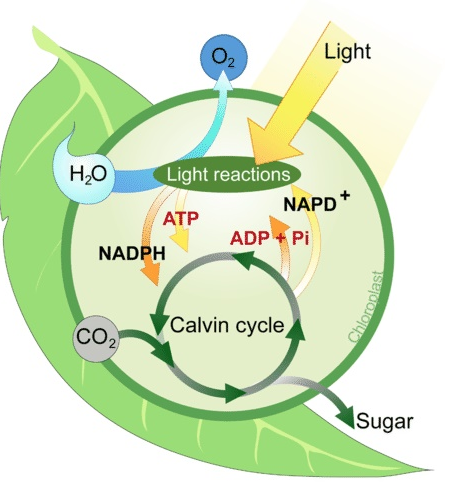
\includegraphics[width=0.5\textwidth]{Figures/CalvinCycle.PNG}
                \caption{Calvin cycle :  The cycle of photosynthesis}
                \label{fig:my_label}
            \end{figure}
            \newpage
            
            \subsection{Pathologies in Plants}
            \hspace{0.5cm}Pathologies in plants refer to any abnormal condition or disease that affects the growth and development of a plant. Pathologies can be caused by a variety of factors, including fungal, bacterial, or viral infections, insect infestations, nutrient deficiencies, and environmental stressors such as drought or temperature extremes.\par
            Plants can be affected by a variety of pathologies that can cause significant damage to crop yields and quality. Some of the most common pathologies include fungal and bacterial infections, viruses, nutrient deficiencies, and environmental stresses such as drought and salinity. Fungal and bacterial infections can cause leaf spots, blights, and wilts, while viruses can lead to stunted growth, yellowing leaves, and poor fruit quality. Nutrient deficiencies can cause a range of symptoms, such as yellowing leaves, poor growth, and reduced yield, depending on the type of nutrient lacking. Environmental stresses can also have a significant impact on plant health, leading to decreased growth, yield, and quality. These pathologies can affect various parts of the plant, such as the leaves, stems, roots, and fruits, and can cause visible symptoms such as discoloration, lesions, and deformations, as well as less visible effects on plant metabolism and physiology. Early detection and diagnosis of these pathologies are essential for effective management and control, as they can significantly impact plant growth, development, and yield.
                \subsubsection{Visible Effects of Plant Pathologies}
                \hspace{0.5cm}In addition to the economic losses that crop industries can experience due to plant pathologies, there are also visible effects that can be observed on the plant itself. For example, plant leaves may exhibit wilting, chlorosis (yellowing), or necrosis (death of tissue). These symptoms can be indicative of a variety of pathologies, including viral, bacterial, and fungal infections. Other visible effects of plant pathologies include reduced growth and yield, as well as deformities in plant structures such as leaves, stems, and fruit. However, not all plant pathologies exhibit visible symptoms, making them difficult to detect. For example, plant viruses can infect plants without causing any obvious signs of disease. This makes it crucial to use non-visible detection methods, such as hyperspectral imaging, to accurately identify the presence of plant pathologies at the tissue level. By detecting the spectral signatures of infected plant tissue, HSI can help farmers and agricultural experts take preventative measures to reduce the spread of plant diseases and optimize crop yield.\par
                \vspace*{1\baselineskip}
                
                 \begin{figure}[h]
                    \centering
                    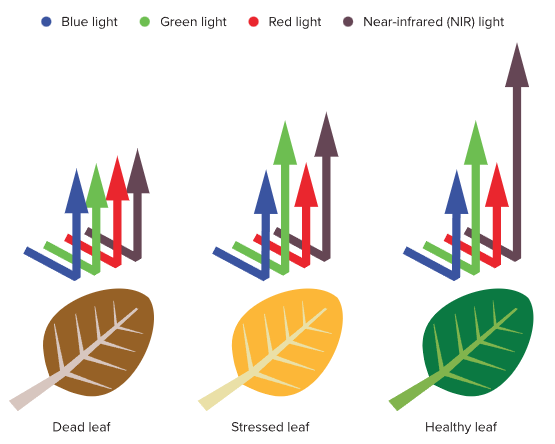
\includegraphics[width=0.6\textwidth]{Figures/leafVis.PNG}
                    \caption{ The color of the leaves in relation to the wavelength of the light absorbed in different states}
                    \label{fig:my_label}
                \end{figure}
                \newpage
                
                \subsubsection{Detection and Diagnosis of Plant Pathologies}
                \hspace{0.5cm}To detect and diagnose plant pathologies, researchers and farmers use a variety of techniques, including visual inspection, laboratory analysis, and remote sensing technologies such as hyperspectral imaging. Hyperspectral imaging uses sensors that can detect wavelengths of light beyond the visible spectrum, allowing researchers to identify subtle changes in plant color and structure that may be indicative of a pathology.\par
                HSI can detect and measure subtle changes in plant growth and development, such as alterations in leaf color, morphology, texture, and plant pigments and nutrients. These changes can be indicators of stress, disease, nutrient deficiencies, or other environmental factors that may impact plant growth. By detecting these changes early on, plant pathologies can be diagnosed and treated more accurately, resulting in better plant health and higher yields.\par
                Specific wavelengths can be used to monitor growth and stress from pathologies inplants. For example, wavelengths in the red and far-red regions of the spectrum areparticularly useful for monitoring plant growth and development, as they are strongly absorbed by chlorophyll and other photosynthetic pigments. Additionally, the blue and green regions of the spectrum are associated with stress responses in plants, and can be used to monitor changes in plant physiology and biochemistry in response to different types of stress. By utilizing these specific wavelengths, researchers and farmers can gain a better understanding of plant health and make informed decisions about crop management practices.\cite{Watterich CB}
                
                \subsubsection{Vegetation Indices in Crop Industry}
                \vspace{1\baselineskip}
                \textbf{Fertilizers}
                
                Fertilizers provide essential nutrients(needed in greater amounts by plants) that affect plant growth and health, such as Nitrogen , Potassium etc.\par
                
                \textbf{Consequences of excess-fertilization }\par
                Over-fertilization on the other hand can cause permanent damage on trees and plants. Excess fertilizer alters the soil by creating high salt concentration and hurt beneficial soil microorganisms. Moreover it can lead to sudden plant growth with insufficient root system to supply the need of water and nutrients of the plant. In addition too much fertilizer can not be naturally dissolved (evaporation & leaching*1occurs) . As a result excess soluble salts*2raise soil salinity and alter soil pH . Finally, excessive fertilization causes plant stress and weakens them, making them susceptible to diseases and insect attacks.\par
                
                \begin{figure}[h]
                    \centering
                    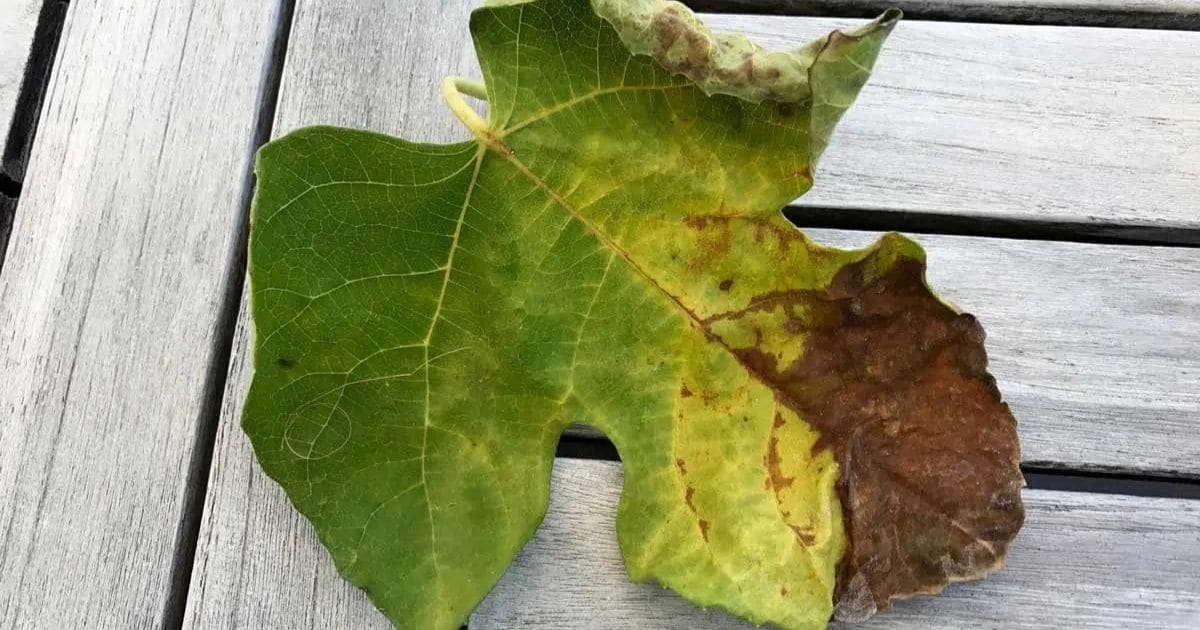
\includegraphics[width=0.7\textwidth]{Figures/excess fertilization.jpg}
                    \caption{Visible effect of excess fertilization}
                    \label{fig:my_label}
                \end{figure}
                
                \newpage
                \textbf{Benefits of quantifying the right amount of fertilizers}\par
                One of the main benefits of quantifying the right amount of fertilizers is improved plant growth and yield. Fertilizers provide essential nutrients such as nitrogen, phosphorus, and potassium, which plants need for growth and productivity. Applying too little fertilizer can lead to nutrient deficiencies, while applying too much can cause nutrient toxicity, both of which can harm plant growth and yield. By quantifying the right amount of fertilizer, farmers can ensure that their crops receive the correct amount of nutrients needed for optimal growth and yield.\par
                Another benefit of quantifying the right amount of fertilizers is improved soil health. Fertilizers can affect soil pH, soil organic matter, and soil microbial activity, which can impact soil health. Applying too much fertilizer can lead to nutrient imbalances, soil acidification, and nutrient runoff, all of which can harm soil health. By quantifying the right amount of fertilizer, farmers can maintain healthy soil that supports plant growth and productivity.\par
                Quantifying the right amount of fertilizers can also help farmers reduce costs and minimize waste. Applying too much fertilizer can be costly, as excess materials may need to be disposed of or can cause environmental problems. By applying the right amount of fertilizer, farmers can reduce the amount of material needed, save money, and reduce waste.\par
                Since NDVI index detects the presence of live green vegetation and is sensitive to chlorophyll absorption we can assess nitrogenlevels. That is because:
                
                \begin{enumerate}
                    \item chlorophyll molecule consists of a central magnesium atom surrounded  by a \textbf{nitrogen-containing}  structure
                    \item nitrogen supply has a large effect on leaf growth because it increases the leaf area of plants
                    \item experiments  have been conducted that verify the strong relation between nitrogen and chlorophyll
                \end{enumerate}
                \vspace*{4\baselineskip}
                
                \begin{figure}[h]
                    \centering
                    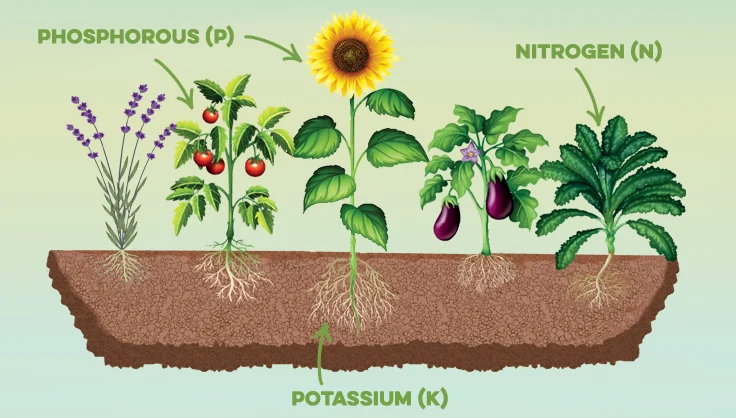
\includegraphics[width=0.8\textwidth]{Figures/fertilizer.png}
                    \caption{Essential plant growth nutrients of fertilizers}
                    \label{fig:my_label}
                \end{figure}
                
                \newpage
                \textbf{Soil Amendments}\par 
                Soil amendments are used to improve the environment for roots and plant growth. That means the improvement of the soil structure, water holding capacity, nutrients availability and living conditions for soil organisms which are important for the plants to grow. Unlike fertilizers, which add nutrients to soil, amendments modify the condition of the soil itself e.g. roots penetrate surrounding soil more easily, water infiltration improves and change soil in ways that affect the availability of plant nutrients.(Note: soil amendments basically help fertilizers do the job they’re intended to do).
                
                \textbf{Consequences of excess use of soil amendments }\par 
                One consequence of excess use of soil amendments is nutrient imbalance. Soil amendments such as manure, compost, and fertilizer can add large amounts of nutrients to the soil. When these nutrients exceed the needs of plants, they can accumulate in the soil, leading to imbalances in the nutrient composition. Excess nutrients can cause environmental problems, such as pollution of water bodies, as they are easily washed away by rainfall or irrigation. Raising soil pH too high sets off a chain of nutrient imbalance.\par
                Another consequence of excess use of soil amendments is soil compaction. Heavy applications of soil amendments can result in the compaction of soil, which reduces the infiltration of water and air into the soil. Compacted soil can lead to poor root development, stunted plant growth, and reduced crop yields.\par
                In conclusion, it is important to use soil amendments in moderation and with care. Excessive use of soil amendments can lead to nutrient imbalances, soil compaction, salinization, and soil contamination. Careful application of soil amendments can help to maintain soil health and support plant growth, while minimizing negative environmental impacts.
                
                \textbf{Benefits of quantifying the right amount of soil amendment }\par
                Soil amendments can improve soil structure by increasing soil porosity, water infiltration, and aeration. This can improve root growth, water retention, and nutrient availability, which can benefit plant growth and overall soil health. Fertilizers, on the other hand, do not improve soil structure.\par
                Some soil amendments, such as lime, can neutralize soil acidity and raise soil pH. This can benefit plant growth by improving nutrient availability and reducing aluminum and manganese toxicity. Fertilizers do not neutralize soil acidity.
                \par
                \begin{figure}[h]
                    \centering
                    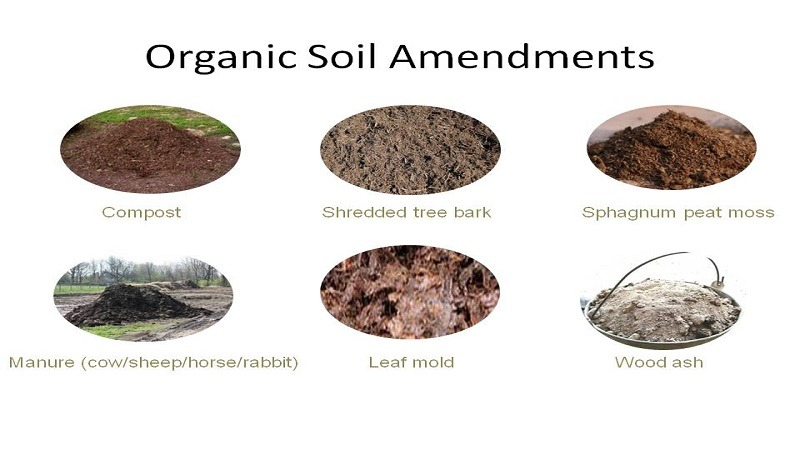
\includegraphics[width=0.8\textwidth]{Figures/soil.jpg}
                    \caption{Organic Soil Amendments}
                    \label{fig:my_label}
                \end{figure}
                \newpage
                
                An increase of GNDVI will be expected from the “no use of soil amendment” plant in comparison with the plant where we used, since it indicates the level of water uptake. Furthermore we expect an increase in GRVI & NDVI index since soil amendment affects plant nutrient intake. 
                
                \subsubsection{Effects of Salinity in Plants}
                The process of plant water uptake is controlled by osmosis, which is the movement of water molecules across a semi-permeable membrane from an area of high water concentration to an area of low water concentration. When salt is present in the soil, it can decrease the water potential of the soil solution, which is the amount of energy required to move water molecules across the membrane. This decrease in water potential can make it harder for plants to absorb water from the soil, as the water molecules must move against a higher concentration of salt ions.\par 
                Salinity is one of the most common abiotic stresses that plants face. Salinity occurs when the concentration of dissolved salts in soil or water exceeds the tolerance threshold of plants. The excess salts create an osmotic imbalance that affects water uptake and stresses the plant. High levels of salinity can also lead to ion toxicity, which can cause leaf burn, necrosis, and other visible symptoms. The effects of salinity on plants can vary depending on the type of plant and the severity and duration of the stress. Some plants are more salt-tolerant than others, but even these plants can suffer reduced growth, yield, and quality when exposed to high levels of salinity. Salinity also affects the nutrient uptake and use efficiency of plants, which can lead to imbalances and deficiencies that further reduce plant health and productivity. Therefore, monitoring and managing salinity is crucial for maintaining plant health and maximizing crop yields.\cite{Munns R}
            \subsection{Vegetation Indices}
            \hspace{0.5cm}Vegetation indices have become an important tool in remote sensing and environmental monitoring, particularly in the field of agriculture and vegetation studies. These indices are mathematical combinations of spectral bands acquired by remote sensing sensors, designed to enhance the contribution of vegetation reflectance and to minimize the effect of other surface features, such as soil or water. By analyzing these indices, researchers can obtain valuable information about plant growth, health, and stress levels, as well as estimate biophysical parameters such as leaf area index, biomass, and vegetation cover.\par
            Moreover, vegetation indices have found applications in the field of plant pathology, as they can be used to detect and monitor diseases and pests in crops. By analyzing changes in vegetation indices over time, researchers can identify abnormal variations in plant growth and detect stress caused by pests or pathogens. Additionally, vegetation indices have been increasingly used in non-destructive techniques to assess plant physiological status, replacing the need for time-consuming and destructive sampling methods used in the past.\par
            In this chapter, we will provide an overview of some of the most widely used vegetation indices, including their theoretical basis, mathematical formulation, and applications. By delving into the analysis of these indices, we will explore how they can be used to provide insights into vegetation dynamics, support decision-making processes in agriculture and forestry management, land use planning, and environmental conservation, as well as their role in plant pathology and non-destructive techniques.
            \vspace*{2\baselineskip}
            \newpage
            
                \textbf{Normalized Difference Vegetation Index (NDVI)}
                \vspace*{1\baselineskip}  
                
                \hspace{0.5cm}The NDVI is a commonly used vegetation index that measures the amount and vigor of green vegetation in an area. The index is calculated using the following formula:\par
                \begin{align*}
                    NDVI = (NIR - Red) / (NIR + Red) \text{\hspace{1cm}(3.1)} 
                \end{align*}
                \vspace*{1\baselineskip}
                where NIR is the near-infrared reflectance value and Red is the red reflectance value. The NDVI ranges from -1 to 1, with values closer to 1 indicating denser and healthier vegetation, while values closer to -1 indicate sparse or stressed vegetation.\par
                The NDVI is widely used in agriculture, forestry, and ecology. In agriculture, it is used to monitor crop growth and detect stress or disease. It can also be used to estimate crop yield and predict harvest timing. In forestry, the NDVI can be used to monitor tree growth and detect areas of deforestation or forest degradation. In ecology, the NDVI is used to measure vegetation cover and assess habitat quality for wildlife.\par
                \vspace*{1\baselineskip}  
                
                \textbf{Enhanced Vegetation Index (EVI)}
                \vspace*{1\baselineskip}  
                
                \hspace{0.5cm}The EVI is a vegetation index that corrects for atmospheric interference and canopy background effects in the NDVI calculation. The formula for calculating the EVI is as follows :\par
                \begin{align*}
                    EVI = 2.5 * ((NIR - Red) / (NIR + 6 * Red - 7.5 * Blue + 1)) \text{\raggedright(3.2)} 
                \end{align*}
                \vspace*{1\baselineskip}
                where NIR is the near-infrared reflectance value, Red is the red reflectance value, and Blue is the blue reflectance value. The EVI has a range from -1 to 1, with higher values indicating denser and healthier vegetation.\par
                The coefficients are used to adjust the contribution of each spectral band to the overall EVI value. Here's a breakdown of what each coefficient represents:\par
                2.5: This coefficient is used to normalize the EVI value so that it falls within a range of -1 to 1. The EVI formula produces values that can range from -∞ to +∞, but by multiplying the result by 2.5, we ensure that the final value is always within the desired range.\par
                6: This coefficient is used to reduce the influence of the red band on the final EVI value. The red band is sensitive to atmospheric scattering, and its contribution to the EVI formula can be affected by the amount of aerosols present in the atmosphere. By reducing the weight of the red band in the formula, the EVI value is less affected by atmospheric interference.\par
                7.5: This coefficient is used to reduce the influence of the blue band on the final EVI value. The blue band is sensitive to atmospheric scattering, and its contribution to the EVI formula can be affected by the amount of aerosols present in the atmosphere. By reducing the weight of the blue band in the formula, the EVI value is less affected by atmospheric interference.\par
                1: This coefficient is used to ensure that the EVI value remains positive. In some cases, the denominator of the EVI formula can be negative, which would result in a negative EVI value. By adding 1 to the denominator, we ensure that the final result is always positive.\par
                The EVI is widely used in agriculture, forestry, and land cover mapping. It is particularly useful in areas with high aerosol content, such as tropical regions, where the NDVI may be affected by atmospheric interference. The EVI can also be used to detect changes in vegetation cover due to land use changes or natural disasters.\par
                \vspace*{1\baselineskip}  
                
                \textbf{Photochemical Reflectance Index (PRI)}
                \vspace*{1\baselineskip}  
                
                \hspace{0.5cm}The PRI is a vegetation index that measures changes in the xanthophyll cycle pigments, which are involved in protecting the photosynthetic machinery from excessive light. The formula for calculating the PRI is as follows:
                \begin{align*}
                    PRI = (Green - Red) / (Green + Red) \text{\hspace{1cm}(3.3)} 
                \end{align*}
                \vspace*{1\baselineskip}
                where Green is the green reflectance value and Red is the red reflectance value. The PRI has a range from -1 to 1, with higher values indicating higher photosynthetic activity.\par
                The PRI is used to monitor vegetation stress and damage, particularly in areas affected by drought, heat stress, or pollution. It can also be used to detect changes in vegetation phenology, such as the onset of senescence or the timing of leaf emergence.\par
                \vspace*{1\baselineskip}  
                
                \textbf{Green/Red Vegetation Index (GRVI)}
                \vspace*{1\baselineskip}  
                
                \hspace{0.5cm}The GRVI is a vegetation index that measures the greenness of vegetation by comparing the reflectance in the green and red bands. The formula for calculating the GRVI is as follows:\par
                \begin{align*}
                    GRVI = Green / Red\ \text{\hspace{1cm}(3.4)} 
                \end{align*}
                \vspace*{1\baselineskip}
                where Green is the green reflectance value and Red is the red reflectance value. The GRVI has a range from 0 to infinity, with higher values indicating denser and healthier vegetation.\par
                The GRVI is commonly used in precision agriculture to monitor crop growth and detect stress or disease. It can also be used to estimate crop yield and predict harvest timing.\par
                \vspace*{1\baselineskip}  
                
                \textbf{Green Normalized Difference Vegetation Index (GNDVI)}
                \vspace*{1\baselineskip}  
                
                \hspace{0.5cm}The Green Normalized Difference Vegetation Index (GNDVI) is a modification of the NDVI, which uses the green band instead of the red band. The GNDVI is calculated as:\par
                \begin{align*}
                    GNDVI = (Green – NIR) / (Green + NIR) \text{\hspace{1cm}(3.5)} 
                \end{align*}
                \vspace*{1\baselineskip}
                \vspace*{1\baselineskip}
                where Green is the green band and NIR is the near-infrared band.\par
                The GNDVI has been shown to be useful for vegetation monitoring in areas where the red band is contaminated by soil, shadows or other non-vegetated features. GNDVI has been applied in studies of forests, grasslands and agricultural crops, such as wheat and maize.\par
                In general, the GNDVI values range from -1 to 1, where positive values indicate vegetation and negative values indicate non-vegetated surfaces.\par
            \vspace*{1\baselineskip}
            Vegetation indices are powerful tools for monitoring vegetation health and growth. NDVI, EVI, PRI, Green/Red and GNDVI are some of the commonly used indices for vegetation analysis.\par
            NDVI is widely used in agriculture and forestry to assess vegetation cover, biomass, and productivity. EVI and PRI are sensitive to plant stress, and have been used for detecting plant stress caused by drought, heat, and other environmental factors. Green/Red is used for measuring chlorophyll content in vegetation, while GNDVI is an alternative to NDVI, useful for areas where the red band is contaminated by nonvegetated features.\par
            The use of vegetation indices in remote sensing has revolutionized our ability to monitor the earth’s vegetation cover and health, and will continue to play a critical role in future research and applications.\par
            \newpage
            \vspace*{3\baselineskip}
            \begin{table}[h]
                \caption{Vegetation Index Applications}
                \vspace*{2\baselineskip}
                \label{tab:veg-index}
                \resizebox{\textwidth}{!}{
                \begin{tabular}{|p{2cm}|p{4cm}|p{5cm}|p{4cm}|}
                    \hline
                    \textbf{Vegetation Index} & \textbf{Application} & \textbf{Used Formula} & \textbf{Description} \\ \hline
                    \centering \vspace*{2\baselineskip}NDVI &\centering \vspace*{2\baselineskip} Agriculture, Forestry &\centering \vspace*{2\baselineskip} $\frac{NIR - RED}{NIR + RED}$ & Measures the difference between near-infrared (NIR) and red light reflectance to estimate the amount and vigor of vegetation. \\ \hline
                    \centering \vspace*{2\baselineskip}GNDVI &\centering \vspace*{2\baselineskip} Agriculture, Ecology &\centering \vspace*{2\baselineskip} $\frac{NIR - GREEN}{NIR + GREEN}$ & Similar to NDVI but uses green light instead of red. Can be used to estimate vegetation cover and photosynthetic activity. \\ \hline
                    \centering \vspace*{2\baselineskip}EVI &\centering \vspace*{2\baselineskip} Coastal Ecosystems &\centering \vspace*{2\baselineskip} $\frac{BLUE - GREEN}{BLUE + GREEN}$ & Measures the difference between blue and green light reflectance to estimate the presence and health of vegetation in coastal ecosystems. \\ \hline
                    \centering \vspace*{2\baselineskip}PRI &\centering \vspace*{2\baselineskip} Terrestrial Ecosystems &\centering \vspace*{2\baselineskip} $\frac{NIR - GREEN}{NIR + GREEN}$ & Measures the difference between near-infrared and green light reflectance to estimate photosynthetic pigments and stress levels in plants. \\ \hline
                    \centering \vspace*{1\baselineskip}Green/Red &\centering \vspace*{1\baselineskip} Agriculture, Horticulture &\centering \vspace*{1\baselineskip} $\frac{GREEN}{RED}$ & Measures the ratio of green to red light reflectance to estimate plant health and stress levels. \\ \hline
                    \centering \vspace*{2\baselineskip}SAVI &\centering \vspace*{2\baselineskip} Agriculture, Forestry &\centering \vspace*{1\baselineskip} $\frac{(NIR - RED)(1+L)}{NIR + RED + L}$ & A modification of NDVI that adjusts for soil brightness, which can affect the accuracy of NDVI in some environments. \\ \hline
                    \centering \vspace*{2\baselineskip}OSAVI &\centering \vspace*{2\baselineskip} Agriculture, Forestry &\centering \vspace*{2\baselineskip} $\frac{NIR - RED}{NIR + RED + a}(1 + a)$ & Another modification of NDVI that adjusts for soil brightness and produces a more accurate estimate of vegetation cover and vigor. \\ \hline
                \end{tabular}}
            \end{table}
            
        \newpage
            \subsection{Remote Sensing in Plants}
            \hspace{0.5cm}Hyperspectral Imaging is a remote sensing technique that involves measuring the properties of an object from a distance. This can be accomplished using a variety of platforms such as satellites, planes, or field-based equipment. In the realm of plant research, remote sensing is applied in three key areas: quality assessment of fruits, vegetation identification, and plant pathology. While the fundamental principles of remote sensing are the same across these areas, there are differences in methodology, available data, and field-specific limitations that must be considered.\par
            To better understand these differences, we can examine the experimental procedures, lighting conditions, and sources of data used in eachapplication. Additionally, it is important to recognize that the economic impact of these fields of research varies based on their relevance to agriculture and food production.\par
            The combination of hyperspectral imaging and other technologies has the potential to bring significant benefits to agriculture and food production. These include reducing fertilizer usage, automating production and packaging, providing targeted treatment for damaging factors, enabling efficient water management, and enhancing the quality of food production.\par Another important application of remote sensing in plant research is the identification and monitoring of vegetation. Hyperspectral imaging can be used to map and quantify vegetation cover, biomass, and growth patterns. This information is critical for understanding ecosystem dynamics, land use planning, and environmental monitoring. Remote sensing can also be used to detect changes in vegetation due to factors such as climate change, land use change, or natural disasters. By analyzing changes in vegetation, scientists can gain valuable insights into the health and sustainability of ecosystems.\par
            In addition to vegetation identification, remote sensing can also be used to detect and monitor plant diseases and pests. Hyperspectral imaging can detect subtle changes in plant reflectance that are indicative of disease or pest infestation before they become visible to the naked eye. This early detection allows for timely interventions and targeted treatment, reducing crop losses and minimizing the use of pesticides. Remote sensing can also be used to monitor the effectiveness of pest and disease management strategies over time, allowing for adjustments to be made as needed.\par
            Overall, remote sensing has the potential to revolutionize the way we understand and manage plant systems. By providing detailed information on plant health, growth, and environmental interactions, hyperspectral imaging can help to optimize agricultural practices, reduce waste, and improve food quality and safety. As technology advances and data analysis techniques improve, remote sensing is likely to become an even more essential tool for plant research and management.In the upcoming chapter, we will explore the research approaches and findings in each of these areas, with a particular focus on plan pathology.\cite{Thenkabail}
                \subsubsection{Advancements in Spectral Imaging for Food Quality Control}
                \hspace{0.5cm}Quality assessment of food is a rapidly growing field due to its importance in society. Consumers have become increasingly concerned about the safety and quality of the food they consume. Consequently, there is a growing interest in providing better food and adhering to high quality standards that people can trust. In addition, automated production processes are becoming more sophisticated and necessary, and technology is being used to ensure that quality standards are met.\par
                In food production, it is essential to differentiate between good and bad produce, such as fruits and meat. Currently, quality control in food production is a human task, which can be tedious and repetitive. There is no room for mistakes, and a certain pace must be maintained throughout the shift. To address this issue, many research groups are focusing on identifying damaged objects using an automated machine that sorts ”good” and ”bad” produce. This technology provides the versatility of a human’s ability to make decisions while also being efficient.\par
                Another reason for implementing spectral imaging in food quality control is its ability to identify different types of damage. By distinguishing between good and bad food, as well as the type of damage, valuable information can be gleaned regarding the source and nature of the problem. For example, Fig.3.12 shows defects and diseases in french fries, illustrating the unique spectral characteristics of a damaged area. Analogous examples can be found in the case of tomatoes, apples, and chickens.\par
                \vspace*{3\baselineskip}
                
                 \begin{figure}[h]
                    \centering
                    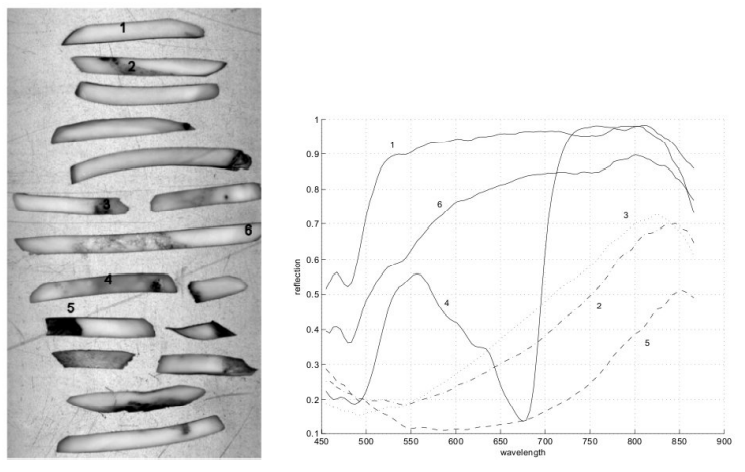
\includegraphics[width=0.72\textwidth]{Figures/potatoParts.PNG}
                    \caption{Several typical French fries defects and diseases with their corresponding spectra. 1=potato flesh, 2=peel, 3=damage,4=greening, 5=external rot, 6=browning}
                    \label{fig:my_label}
                \end{figure}
                
                Initial attempts used simple RGB cameras and computers in a basic machine vision system to assess the quality of produce. The system showed promise, but lacked the required level of accuracy. However, researchers [18], [9], and [19] found that hyperspectral imaging approaches outperformed RGB images since many defects are not visible in color images. Hyperspectral imaging provides more information, allowing researchers to differentiate between different states of maturity, types of damage, diseases, and defects. Labeling and classification accuracy is significantly improved.\par
                While applying hyperspectral imaging in food production has been proven effective, there are some drawbacks. The system must be able to provide real-time results and process a vast amount of information to maintain an acceptable rate in the distinguishing machine, successfully and efficiently identifying stress factors and defects. Researchers are currently focusing on improving accuracy by leveraging various spectra signatures, such as the ripeness of tomatoes, certain stress impacts, and more. The following table (Tab.1) depicts various attempts at food quality evaluation, taken from \cite{DuSun}.\par
                
                \begin{table}[h]
                \centering
                \caption{CCD Camera Applications for Food Quality Evaluation}
                \vspace*{2\baselineskip}
                \label{tab:food-quality}
                \resizebox{\textwidth}{!}{
                \begin{tabular}{|p{2cm}|p{4cm}|p{5cm}|p{4cm}|}
                \hline
                    
                    \centering \textbf{Category} &\centering \textbf{Products} &\centering \textbf{Applications} & \textbf{\hspace{24pt} References} \\ \hline
                    \centering \vspace{0.2cm}Fishery & \centering \vspace{0.2cm} Bivalve Crassostrea Fish &Study of larval growth, Detection of hinge lines, Sorting fish & Pontual et al. (1998), Jung and Fred (2002), Zion et al. (1999) \\ \hline
                     \centering \vspace*{1\baselineskip}Fruit & \centering \vspace*{1\baselineskip} Apple Cherry Orange Pistachio nuts & Defect segmentation, Analysing fruit shape, Location and characterization of the stem-calyx area, Detection of early split & Leemans et al. (1999), Beyer et al. (2002), Ruiz et al. (1996), Pearson and Slaughter (1996) \\ \hline
                     \centering \vspace{0.1cm}Grain & \centering \vspace{0.1cm}Rice Wheat & Quality classification, Classification & Wan et al. (2002), Utku and Koksel (1998) \\ \hline
                     \centering \vspace*{1\baselineskip}Meat & \centering \vspace*{1\baselineskip} Beef Pork Poultry carcasses & Using image texture features as indicators of tenderness, Color evaluation, Classification & Li et al. (1999), Lu et al. (2000), Park et al. (2002) \\ \hline
                     \centering \vspace*{0.1cm}Vegetable & \centering \vspace*{0.1cm} Asparagus Chicory & Defect inspection, Study of visual preference & Rigney et al. (1992), Coppenolle et al. (2002) \\ \hline
                     \centering \vspace*{2\baselineskip}Other & \centering \vspace*{1\baselineskip} Cheese Noodle Pizza Sausage & Evaluation of the functional properties, Influence of sprout damage on appearance, Quality evaluation, Estimation of sensory properties & Wang and Sun (2001), Hatcher and Symons (2000), Sun and Brosnan (2003a, 2003b), Ioannou et al. (2002) \\ \hline
                \end{tabular}}
                \end{table}
                
                Overall, implementing hyperspectral imaging technology in food quality assessment has the potential to significantly improve food safety and quality. By automating the process, reducing human error, and providing valuable information on the source and nature of defects, hyperspectral imaging can play a critical role in the future of food production.\cite{Kumar}
                \newpage
                
                \subsubsection{Advances in Vegetation Identification Using Remote Sensing Techniques}
                \hspace{0.5cm}Vegetation Identification using remote sensing techniques has emerged as an important field for extracting valuable information about the quality and physiological status of plant matter. By analyzing the reflectance and absorbance spectra of chlorophyll and carotenes, researchers have been able to develop methods for assessing chlorophyll content in leaves quickly and non-destructively. Large-scale projects like AVIRIS,MODIS and Landsat-8 have successfully used remote sensing to identify vegetation over vast areas.\par

                \begin{figure}[htp]
                    \centering
                    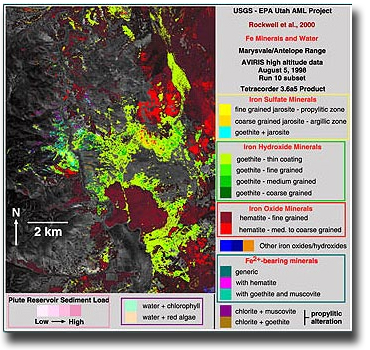
\includegraphics[width=0.5\textwidth]{Figures/AVIRIS.png}
                    \caption{Example of research conducted by the United States Geological Survey using AVIRIS data.}
                    \label{fig:aoua}
                \end{figure}
            
                Airborne remote sensing has the advantage of covering large areas, but still faces limitations in terms of resolution and accuracy. However, it remains a promising tool for vegetation identification and disease diagnosis, and has proven more effective than satellite remote sensing in certain applications. As research continues in this field, we can expect to see continued advancements in the use of remote sensing for vegetation identification and assessment, as well as disease diagnosis and monitoring.\par
                While remote sensing has proven effective for identifying and discriminating different types of vegetation, efforts are being made to expand its capabilities and improve the quality of information extracted. Spectral bands that show high correlation with chlorophyll concentration are being used to develop indices that can estimate pigment concentrations directly from spectral information. Several indices have been defined, such as the Enhanced Vegetation Index (EVI), that have been validated across different species. However, there is still debate over which bands provide the best results, since spectral responses can differ between species and are also influenced by factors like leaf structure and physiology.\par
                To develop indices that are more generic and provide immunity across species, it is crucial to define means of estimating concentrations and pathologies that are not as strongly affected by such factors. In addition, remote sensing techniques are increasingly being used to diagnose plant pathologies, such as nutrient deficiencies, water stress, and disease outbreaks. By analyzing spectral signatures associated with specific pathologies, researchers have been able to develop methods for detecting and monitoring these conditions over large areas. In the next subchapter we will analyze how spectroscopy is used in crop industry to prevent major loses via early identification of contagious or not pathologies.
                \newpage
            \subsection{Pigments}
            \hspace{0.5cm}Pigments play a crucial role in the coloration of fruits, and their degradation or production can indicate the ripening process. Chlorophyll, a green pigment responsible for photosynthesis, is found in most fruits and absorbs blue and red light while reflecting green light. As fruits ripen, the degradation rate of chlorophyll is enhanced, leading to color changes that are sometimes due to the production of carotenoids or flavonoids, two other common groups of pigments in nature responsible for yellow to red and red or purple colors, respectively.\par
            \vspace*{1\baselineskip}
            
            \begin{figure}[h]
                \centering
                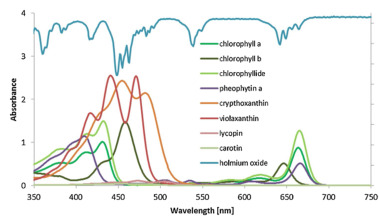
\includegraphics[width=0.7\textwidth]{Figures/pigmentWav.PNG}
                \caption{ Absorption spectra of pigments}
                \label{fig:my_label}
            \end{figure}
            
            \vspace*{1\baselineskip}
            Researchers have developed various methods to predict the ripening process of fruits based on pigment analysis. For instance, Saputro et al. (2018) used hyperspectral imaging to detect the ripening of bananas by predicting the amount of chlorophyll pigment in the fruit peel. The study yielded good results in predicting chlorophyll content and determining the ripening level of bananas. Similarly, Permata et al. (2017) reported similar results in predicting the ripening level of bananas by estimating carotenoid pigment. In another study, Cho et al. (2021) used hyperspectral imaging to predict anthocyanins, a pigment responsible for the red coloration of strawberries, at different stages of maturity. The study achieved high accuracy using spectral information to create spatial distribution maps of the pigment on the surface of the strawberries.\par
            Overall, the analysis of pigments in fruits can provide valuable information about the ripening process and the fruit’s nutritional content. The use of hyperspectral imaging and other techniques can help to accurately predict the ripening level of fruits and detect changes in their pigmentation. These methods could have important applicationsin the food industry and could help to reduce food waste by improving fruit quality control.
            \newpage
        \section{Experiment \& Research}
            \setcounter{figure}{0}
            The upcoming section will outline the experimental methodology employed in the study, including the equipment used and the enhancements made to the Classification Algorithms and the Software utilized by the HSI system.
            \subsection{Hyperspectral Imaging System }
                    \hspace{0.5cm}Our experiment involved setting up two groups of tomato plants: one group was subjected to excess salinity, while the other group was not. The purpose of this experiment was to determine if spectroscopy could prevent the stressful effects of salinity on plants. To ensure accuracy, we added balances under each plant to ensure they had the same amount of soil, and water was carefully added in precisely measured amounts. After carefully monitoring the plants for 17 days using the spectroscopy tool, our measurements mainly focused on the plant’s branches rather than its leaves. The equipment used in this experiment will be further analyzed later in this chapter.
                    \vspace*{1\baselineskip}
                    
                    \textbf{Experiment Initialization}
                    \vspace*{1\baselineskip}
                    
                        \hspace{0.5cm}The first stage of the experiment was conducted at Mediterranean Agronomic Institute of Chania (MAICH), with a specific area being designated for this purpose. The correct initialization of the experiment was paramount, and so the lighting for the plants was carefully set up since they were not exposed to sunlight. In order to ensure consistency, exact same amount of soil was measured and used for each plant, for both the groups that were to receive salinity and those that were not. The same variety of tomato was planted in each pot, and scales were used to assess the homogeneity of the plants. Although weight may not necessarily indicate uniformity, the scales allowed us to verify that each plant received the same amount of soil and water. Salinity was then added to the first group of plants, while the second group was kept as a control.\par
                        To keep track of each plant and its treatment, small tags were attached to their pots with labels indicating the group and plant number. The plants subjected to excess salinity were labeled ExcS(N) and the plants that were not SalC(N), where N represents the plant number (1, 2, or 3). Moreover, ExcS-iW & SalC-iW are the same groups but over exposed to water where i is the number of the plant and W stands for water. By using these labels, we were able to accurately monitor the condition of each plant throughout the experiment.\par
                        \vspace*{1\baselineskip}
                        $\cdot $ExcS$: ExcessSalinity \par
                        \vspace*{1\baselineskip}
                        $\cdot $SalC$: SalinityControl \par
                        \vspace*{1\baselineskip}
                        $\cdot $ExcS-W$: ExcessSalinity \& Water \par
                        \vspace*{1\baselineskip}
                        $\cdot $SalC-W$: SalinityControl,Excess Water \par
                        \newpage
                        \vspace*{1\baselineskip}
                        
                    \textbf{Hyperspectral Imaging Technology for In-situ Diagnosis}
                    \vspace*{1\baselineskip}
                    
                        \hspace{0.5cm}HSI systems, or hyperspectral imaging systems, consist of a camera that can detect and analyze the spectral properties of objects and surfaces in great detail.     These systems can be used for a variety of applications, including crop monitoring and stress detection.\par
                        The HSI system used in our study is QCELL’s PhenoCheck camera and is an electrooptic device that is specifically designed for in situ monitoring of crops. It enables   real-time monitoring of plant health and stress detection, making it a valuable tool for precision agriculture. The system features a powerful spectral imaging system that can capture multiple critical spectral bands simultaneously and at video rate.
                        \textbf{Some of QCELL's PhenoCheck camera key features are :}\par
                        \renewcommand{\theenumi}{\roman{enumi}}%
                        \begin{enumerate}
                            \item  Imaging spectral range: 400-1100nm
                            \item  Illumination spectral range: broad-band 400-1100nm and narrow-band 365nm or 405nm for fluorescence excitation
                            \item  Illumination technology: diffusive dome Illumination eliminating glare
                            \item  Imaging modes: reflectance and fluorescence
                            \item  Real-time simultaneously displayed images: 410nm, 464nm, 542nm, 639nm, 780nm, 880nm, (30nm FWHM), color reflectance, color fluorescence, vegetation index maps        and unsupervised classification maps.
                            \item  HyperSpectral Imaging: 50 bands with machine learning spectral estimation
                            \item  Spatial resolution: 6 megapixels for every acquired/estimated image and map
                            \item  Field-of-View: 23X15 mm
                            \item  Magnification X30 and X50 (with window magnification)
                            \item  Hours of battery operation: 4
                            \item  Weight: 800g
                            \end{enumerate}
                        One of the system’s primary advantages is its ability to operate in dual mode, allowing for both diffuse reflectance and fluorescence imaging in the visible and near-infrared spectral bands. It provides real-time color images, spectral images, vegetation index heat maps, and spectral maps side-by-side, which provide objective and quantitative information for stress detection and crop analysis.\par
                        The HSI system used in our study, QCELL’s PhenoCheck camera , is capable of detecting and classifying plant pathologies, nutrient and water stress, and fruit ripening assessment in situ. By utilizing various spectral bands and vegetation indices, it can accurately and objectively detect any abnormalities or stress factors affecting crops. One of the commonly used vegetation indices in the crop industry is the Normalized Difference Vegetation Index (NDVI), which measures the difference between near-infrared (NIR) and red light reflected by plants.\par
                        Apart from its imaging capabilities, the system can perform in situ classification for plant pathologies, water and nutrient stress, and fruit ripening assessment. It is a plug-and-play system that can be easily interfaced with a dedicated tablet PC, making it convenient for on-the-spot diagnostics.\par
                        Overall, the PhenoCheck camera offers a comprehensive solution for crop monitoring and stress detection, utilizing common vegetation indices used in the crop industry via its usefull function for live classification. Its advanced features and capabilities make it an essential tool for precision agriculture and crop management.
                    \vspace*{1\baselineskip}
                    
                    \textbf{Analysis}
                    \vspace*{1\baselineskip}
                    
                        \hspace{0.5cm}Following the setup of our experiment and the installation of the HSI equipment, we proceeded to take measurements for each plant group, focusing mainly on the stem since it plays a crucial role in plant growth. Our measurements included live monitoring of the vegetation indices provided by the HSI system. Experiment was focused on finding deficiencies between two groups of tomato plants via spectral classification and mapping. The data collected from the measurements were saved in the HSI system and later analyzed using a self-developed clustering software at QCELLS headquarters. The following chapter will provide a detailed examination of the software and algorithms developed during the experiment to classify the data for further analysisspo.
                        
                    \subsection{Software \& Algorithm Development}
                    This sub-chapter focus on the software developed for analyzing the results of our experiment and was implemented using the Qt Framework. In the following sections, we will elaborate on the modifications made to the k-means classification algorithm. Specifically, we implemented a variant of the algorithm that was well-suited for our experiment and made several adjustments to reduce the execution time of the algorithm, which will be discussed in detail.\par
                    As it is mentioned in the previous chapter K-Means is a clustering algorithm that separates our data into k groups. The way we select the number of groups in which our data will be divided is either manually selected (the user defines the number of different groups) or through a convention that answers the question: when do we consider creating a new group of data (new cluster) and we are not satisfied with the existing clusters?\par
                    The primary challenge with the first option of manually selecting the number of clusters for K-Means is that in scenarios such as research experiments, the optimal number of clusters may not be known beforehand. To overcome this, the K-Rms algorithm was developed, which involves a small complexity algorithm to compare data and determine the appropriate number of clusters.
                    
                    \begin{align*}
                        RMSE = \sqrt{\frac{\sum_{i=Channel_1}^{i=Channel_N} (Pixel[i]-Centroid[i])^2}{N}} && \text{(4.1)} 
                    \end{align*}
                    
                    The K-Rms algorithm begins by randomly selecting a point or pixel as the first cluster. Next, it compares this cluster to the remaining points or pixels and evaluates whether the RMSE distance is bigger or lesser from a predetermined parameter value. As the value increases, the algorithm will produce fewer clusters since it becomes more challenging to identify greater distances between points in each iteration. If the RMSE distance is greater than the predetermined value, a new cluster is created. The algorithm then repeats the same process by comparing the remaining points or pixels to the first and new clusters. Only if the RMSE distance of a point is larger than that of all existing clusters will a new cluster be created.This modification to the original K-Means algorithm was essential in identifying any underlying patterns or unexpected results that may not be immediately apparent to the naked eye over time.\par
                    \newpage
                    One major disadvantage of using K-Rms is that it can produce noise clusters, which greatly affects the execution time and performance of the algorithm. This is because noise pixels have a spontaneous and unpredictable spectrum, which can be mistakenly taken as clusters because their rmse value may be larger than that of the existing clusters. By lowering the value of rmse, we can achieve a more detailed classification, but at the cost of creating even more noise clusters for the rest of the algorithm's execution. To mitigate this issue, a simple method can be implemented to remove clusters that contain only a small percentage of points before running the second part of the algorithm. However, this also means that krms may not be suitable for immediate use in situ applications and instead requires processed data where noise has been eliminated prior to being fed into the K-Rms algorithm.A comparative study was conducted to evaluate the execution time of K-Rms centroids initialization,  the performance of both algorithms and lastly the execution time of the algorithm using various similarity measures in regards with the rmse value.\par
                    \vspace*{2\baselineskip}
                    
                    
                    \begin{figure}[h]
                        \centering
                        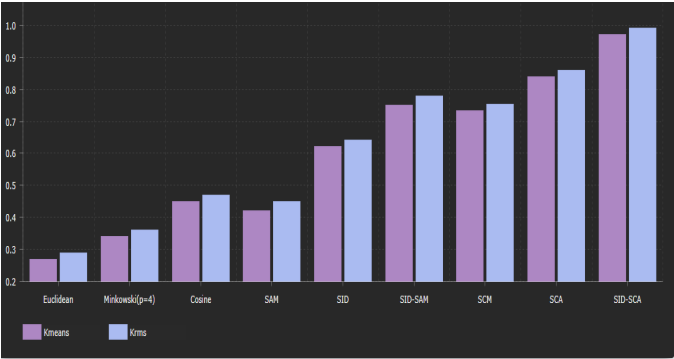
\includegraphics[width=1\textwidth]{Figures/km-krms.PNG}
                        \caption{Bar chart comparing the execution time per iteration of KMeans \& Krms for broadly used similarity measures}
                        \label{fig:my_label}
                    \end{figure}
                    
                    As anticipated, Krms was found to take more time than Kmeans for all similarity measures, owing to the additional algorithm required for initializing centroid clusters. This algorithm is more time-consuming than any of the initialization methods used in Kmeans, including random, farthest, and kmeans++. In this comparison study, KMeans centroids were initialized using kmeans++ method.\par
                    \vspace*{1\baselineskip}
                    
                    
                
                    The exponential increase in execution time in accordance to the the decrease in RMSE values are observed due to the formation of new centroids in response to small differences from existing centroids. As the number of centroids increases with each iteration, the computational effort required to compare each point-pixel to the new centroids also increases, leading to longer execution times.\par
                    
                    \begin{figure}[h]
                        \centering
                        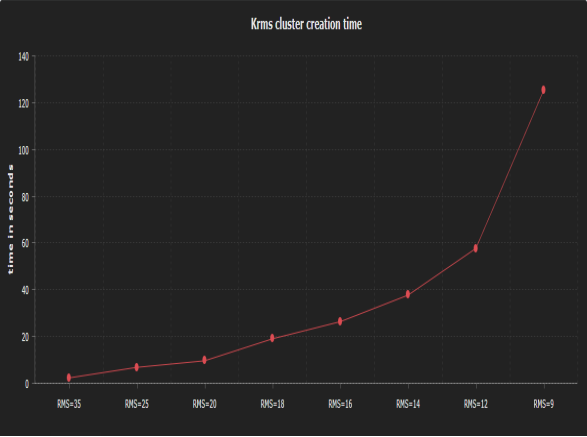
\includegraphics[width=0.8\textwidth]{Figures/KrmsClusterCreationTime.PNG}
                        \caption{K-Rms centroids initialization time}
                        \label{fig:my_label}
                    \end{figure}
                    
                    \begin{figure}[h]
                        \centering
                        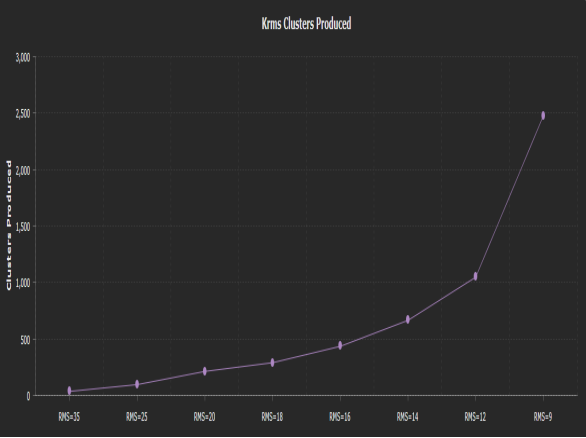
\includegraphics[width=0.8\textwidth]{Figures/K-RmsClusterProd.PNG}
                        \caption{Clusters produced for the various values of RMSE}
                        \label{fig:my_label}
                    \end{figure}
                    
                    \begin{figure}[h]
                        \centering
                        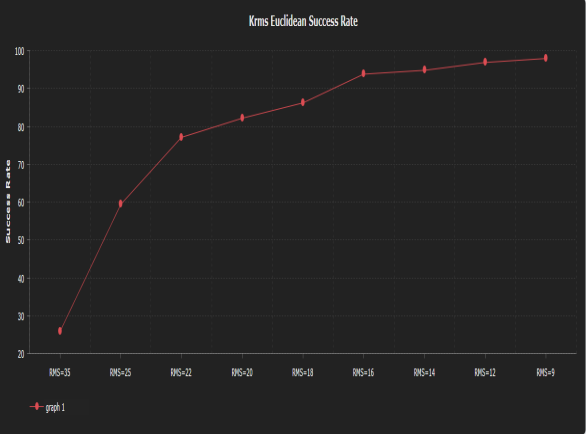
\includegraphics[width=0.8\textwidth]{Figures/krmsEuclSuc.PNG}
                        \caption{K-Rms Euclidean success rate}
                        \label{fig:my_label}
                    \end{figure}
                    
                    \begin{figure}[h]
                        \centering
                        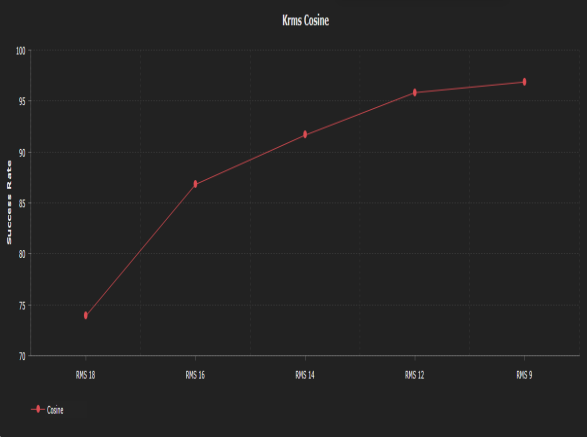
\includegraphics[width=0.8\textwidth]{Figures/krmsCosSuc.PNG}
                        \caption{K-Rms Cosine success rate}
                        \label{fig:my_label}
                    \end{figure}
                    
                    \begin{figure}[h]
                        \centering
                        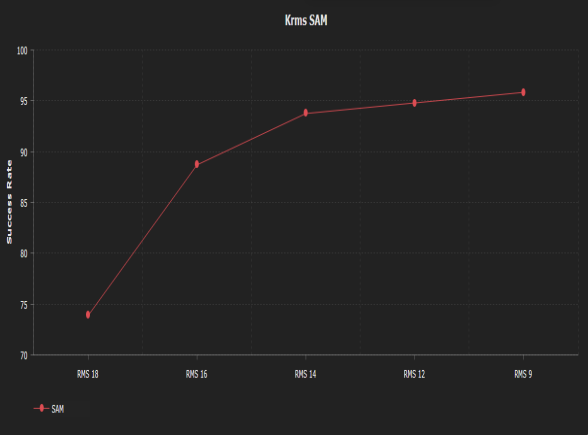
\includegraphics[width=0.8\textwidth]{Figures/krmsSamSuc.PNG}
                        \caption{K-Rms SAM success rate}
                        \label{fig:my_label}
                    \end{figure}
                    
                    \begin{figure}[thb]
                        \centering
                        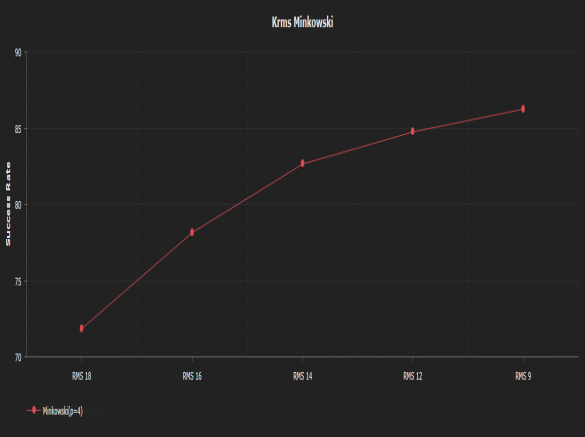
\includegraphics[width=0.8\textwidth]{Figures/krmsMink.PNG}
                        \caption{K-Rms Minkowsky success rate}
                        \label{fig:my_label}
                    \end{figure}
                    \clearpage
                    \newpage
                    After the initializing step is complete, both for K-Means algorithm and the KRms algorithm which was used in this experiment, a 3D array is produced. The rows of this array represent the number of centroids or clusters produced which as we mentioned for K-Means is predefined and for KRms is not, while the columns represent the spectra used in the analysis. The size of the columns depends on the number of wavelengths in the hyperspectral cube that was subjected for analysis. The third dimension of the array contains the intensity values in each wavelength of the corresponding pixel which was selected as representative of the cluster after the centroid initialization process.\par
                    In the following step, the 3D array of clusters obtained from the previous step is passed as a parameter to initiate the deletion of "noise clusters". As the number of clusters increases or the RMSE value decreases, more noise clusters tend to emerge. These noise pixels have unpredictable spectra, characterized by sudden and sharp changes, which may easily be mistaken for a separate cluster. To solve this issue, a minimum percentage of the total number of pixels present in the image is set as a threshold for cluster selection. If a cluster fails to meet this minimum criterion, it is considered as noise and removed from the final classification result.\par
                    By employing the above approach, the likelihood of misclassification of noise pixels as a separate cluster is significantly reduced. The minimum percentage threshold acts as a safeguard to ensure that only well-defined and significant clusters are retained in the classification result. It also helps in reducing the computational complexity and memory usage by avoiding the inclusion of noise clusters in the final classification output. The process of noise cluster removal is an essential step in the classification process, which significantly enhances the overall accuracy and robustness of the classification algorithm.\par
                    After the initial assignment of pixels to clusters, the next step of the K-Means algorithm is to re-calculate the centroids' values. This is necessary because the centroids' values change after every iteration, and recalculating them ensures that the right pixels are assigned to the correct cluster. The number of iterations needed to achieve the desired accuracy can vary, and there are various methods and research papers available that explain how to determine the optimal number of clusters.
                    In the K-Rms algorithm, a function is called after each iteration of centroid reassignment to check if the cluster values have changed from the previous iteration. If the values remain the same, it indicates that the algorithm has converged, and no further iterations are required. This approach helps to optimize the algorithm's performance and speed up the classification process.\par
                    
                    For Instance where RMSE = 40
                    
                    
                    \begin{figure}[h]
                        \centering
                        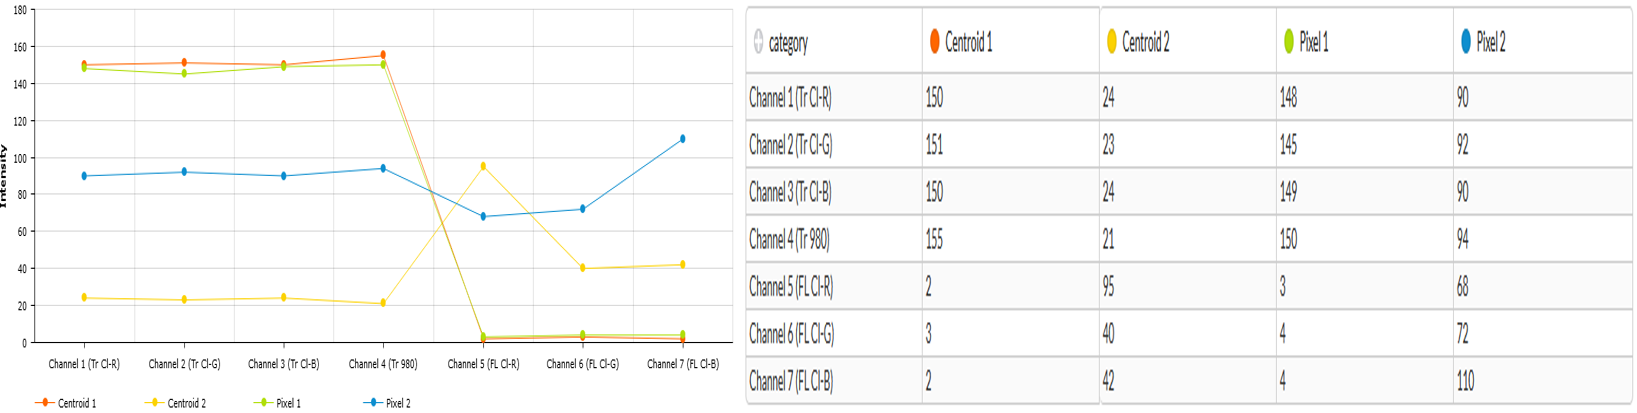
\includegraphics[width=1\textwidth]{Figures/SpectraChannels.PNG}
                        \caption{Spectrum of Centroids \& Pixels}
                        \label{fig:my_label}
                    \end{figure}
                    
                    
                    Figure 4.8 displays the spectra of centroid 1, centroid 2, pixel 1, and pixel 2. The spectrum of centroid 2 is remarkably similar to that of pixel 2, indicating that it will be assigned to the corresponding cluster. However, it is uncertain which centroid pixel 2 belongs to, and thus the RMSE formula (4.1) is utilized to determine which centroid is closer to pixel 2 or even if we have to create another cluster.
                    \newpage
                    \vspace*{3\baselineskip}
                    
                    \begin{table}[h]
                      \centering
                      \caption{Centroids \& Pixel 1 values}
                      \vspace*{2\baselineskip}
                      \label{tab:result-table}
                      \renewcommand{\arraystretch}{2.5} % adjust cell height
                      \resizebox{\textwidth}{!}{
                      \begin{tabular}{|p{2cm}|p{3cm}|p{3cm}|p{3cm}|p{3cm}|p{3cm}|p{3cm}|p{3cm}|}
                        \hline
                        \textbf{} & \centering \textbf{Channel 1} & \centering  \textbf{Channel 2} & \centering \textbf{Channel 3} & \centering \textbf{Channel 4} & \hspace{0.2cm} \textbf{Channel 5} & \hspace{0.2cm} \textbf{Channel 6} & \hspace{0.2cm} \textbf{Channel 7} \\ 
                        \hline
                        \centering Pixel 1 & \hspace*{1.1cm} 148 &  \hspace*{1.1cm} 145 & \hspace*{1.1cm} 149 &  \hspace*{1.1cm} 150 &  \hspace*{1.1cm} 3 &  \hspace*{1.1cm} 4 &  \hspace*{1.1cm} 4 
                        \\
                        \hline
                        
                        \centering Centroid 1 &  \hspace*{1.1cm} 150 &  \hspace*{1.1cm} 151 &  \hspace*{1.1cm} 150 &  \hspace*{1.1cm} 155 &  \hspace*{1.1cm} 2 &  \hspace*{1.1cm} 3 &  \hspace*{1.1cm} 2  
                        \\
                        \hline
                        
                        \centering Centroid 2 &  \hspace*{1.2cm} 24 &  \hspace*{1.2cm} 23 &  \hspace*{1.2cm} 24 &  \hspace*{1.2cm} 21 &  \hspace*{1.1cm} 95 &  \hspace*{1.1cm} 40 &  \hspace*{1.1cm} 42  \\
                        \hline
                       \end{tabular}}
                    \end{table}
                    \begin{itemize}
                        \item Calculation of RMS for Pixel 1 and Centroid 1 $<$ 40
                        \item Calculation of RMS for Pixel 1 and Centroid 2 $>$ 40
                    \end{itemize}
                    
                    As the RMS distance must be greater than 40 for all Centroids, which is not the case for Pixel 1 as we can see, Pixel 1 will not become a Centroid and thus a new Cluster will not be created.
                    \vspace*{3\baselineskip}
                    
                    \begin{table}[h]
                      \centering
                      \caption{Centroids \& Pixel 2 values}
                      \vspace*{2\baselineskip}
                      \label{tab:result-table}
                      \renewcommand{\arraystretch}{2.5} % adjust cell height
                      \resizebox{\textwidth}{!}{
                      \begin{tabular}{|p{2cm}|p{3cm}|p{3cm}|p{3cm}|p{3cm}|p{3cm}|p{3cm}|p{3cm}|}
                        \hline
                        \textbf{} & \centering \textbf{Channel 1} & \centering  \textbf{Channel 2} & \centering \textbf{Channel 3} & \centering \textbf{Channel 4} & \hspace{0.2cm} \textbf{Channel 5} & \hspace{0.2cm} \textbf{Channel 6} & \hspace{0.2cm} \textbf{Channel 7} \\ 
                        \hline
                        \centering Pixel 2 & \hspace*{1.1cm} 90 &  \hspace*{1.1cm} 92 & \hspace*{1.1cm} 90 &  \hspace*{1.1cm} 94 &  \hspace*{1.1cm} 68 &  \hspace*{1.1cm} 72 &  \hspace*{1.1cm} 110 
                        \\
                        \hline
                        
                        \centering Centroid 1 &  \hspace*{1.1cm} 150 &  \hspace*{1.1cm} 151 &  \hspace*{1.1cm} 150 &  \hspace*{1.1cm} 155 &  \hspace*{1.1cm} 2 &  \hspace*{1.1cm} 3 &  \hspace*{1.1cm} 2  
                        \\
                        \hline
                        
                        \centering Centroid 2 &  \hspace*{1.2cm} 24 &  \hspace*{1.2cm} 23 &  \hspace*{1.2cm} 24 &  \hspace*{1.2cm} 21 &  \hspace*{1.1cm} 95 &  \hspace*{1.1cm} 40 &  \hspace*{1.1cm} 42  \\
                        \hline
                       \end{tabular}}
                    \end{table}
                    \begin{itemize}
                        \item Calculation of RMS for Pixel 2 and Centroid 1 $>$ 40
                        \item Calculation of RMS for Pixel 2 and Centroid 2 $>$ 40
                    \end{itemize}
                    
                    The RMS distance between Pixel 2 and all Centroids is greater than 40 in each case. Therefore, Pixel 2 will become Centroid 3, where Centroid 3 will include the values of Pixel 2 for each Channel, and a new Cluster will be created.\par
                    As it is mentioned in KMeans subchapter the next step after initialization is to assign all pixels to their "closest" centroid. The closest centroid is defined as the centroid with the smallest distance difference from the respective pixel.After all the pixels are assigned to the closest cluster the mean value of each channel is calculated for each Centroid, based on the assigned pixels.
                    
                    \newpage
                    \begin{figure}[h]
                        \centering
                        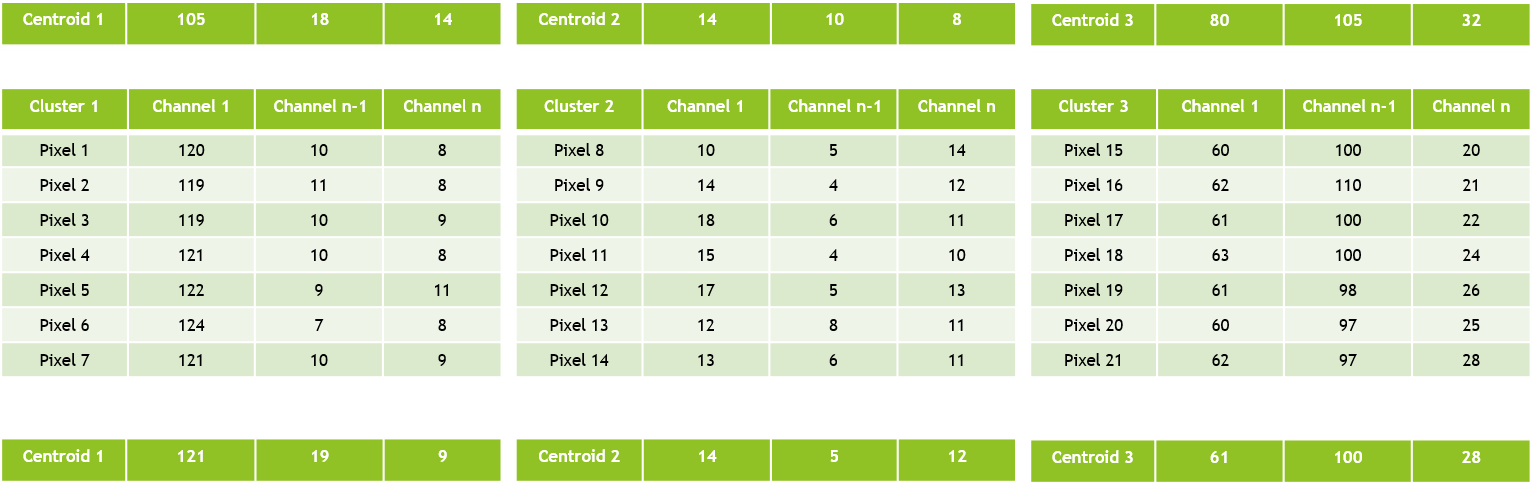
\includegraphics[width=\textwidth]{Figures/pinaxCentrs.png}
                        \caption{Centroids Recalculation}
                        \label{fig:my_label}
                    \end{figure}
                    
                    Finally, we repeat steps 2 and 3 n times, as by recalculating the means in each iteration, different pixels are assigned to the centroids compared to those assigned in the previous iteration.
                    
        \section[Results \& Conclusions]{}
            \setcounter{figure}{0}
                \begin{landscape} % This starts the landscape page for the Results chapter
                    \subsection{Data}\par
                    \vspace*{-3.8\baselineskip}
                    \hrule
                    
                    \thispagestyle{lscape}
                    \pagestyle{lscape}
                    
                    \textbf{Gradient-Based Color Mapping for Vegetation Indices}
                    \vspace*{3\baselineskip}
                    
                    \begin{tabularx}{\linewidth}{>{\arraybackslash}X>{\arraybackslash}X}
                    \toprule
                    \textbf{\hspace{2cm} Vegetation Index} & \hspace{4cm}  \textbf{Color Mapping} \\
                    \midrule
                    
                    \vspace*{3\baselineskip}
                    \textbf{NDVI} (Normalized Difference Vegetation Index) & \vspace*{3\baselineskip} \begin{minipage}[t]{\linewidth}
                                                                                                            \vspace{-10pt}
                                                                                                            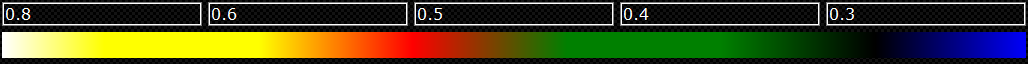
\includegraphics[width=\linewidth]{Figures/1.png}
                                                                                                         \end{minipage}\\
                    \vspace*{3\baselineskip}
                    \textbf{EVI} (Enhanced Vegetation Index) & \vspace*{2\baselineskip} \begin{minipage}[t]{\linewidth}
                                                                                                     \vspace{0pt}
                                                                                                     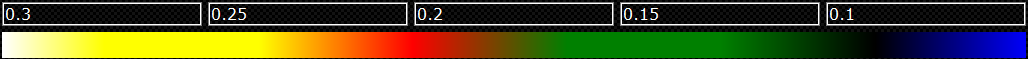
\includegraphics[width=\linewidth]{Figures/2.png}
                                                                                                  \end{minipage} \\
                    \vspace*{3\baselineskip}
                    \textbf{PRI} (Photochemical Reflectance Index) & \vspace*{1.7\baselineskip} \begin{minipage}[t]{\linewidth}
                                                                                                     \vspace{0pt}
                                                                                                     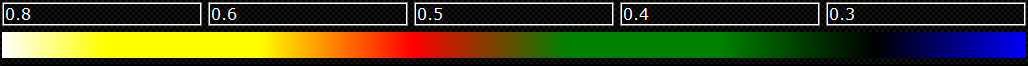
\includegraphics[width=\linewidth]{Figures/3.png}
                                                                                                  \end{minipage}\\
                    \vspace*{3\baselineskip}
                    \textbf{GRVI} (Green-Red Vegetation Index) &\vspace*{2\baselineskip} \begin{minipage}[t]{\linewidth}
                                                                                                     \vspace{0pt}
                                                                                                     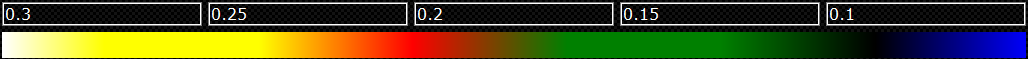
\includegraphics[width=\linewidth]{Figures/2.png}
                                                                                                  \end{minipage}
                                                \\
                    \vspace*{3\baselineskip}
                    \textbf{GNDVI} (Green Normalized Difference Vegetation Index) & \vspace*{2\baselineskip} \begin{minipage}[t]{\linewidth}
                                                                                                                   \vspace{0pt}
                                                                                                                   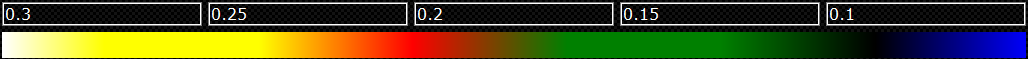
\includegraphics[width=\linewidth]{Figures/2.png}
                                                                                                                \end{minipage}\\   
                    \addlinespace[55] 
                    %\bottomrule
                    \end{tabularx}
                    \newpage
                   \vspace*{-3.8\baselineskip}
                    \hrule
                    \vspace*{3\baselineskip}
                    
                    \begin{center}
                        \textbf{Comparison study between salinity and control plants from 31st of March to 16th of April}
                    \end{center}
                    
                    \begin{figure}[h]
                      \centering
                      \begin{subfigure}[b]{0.72\textwidth}
                        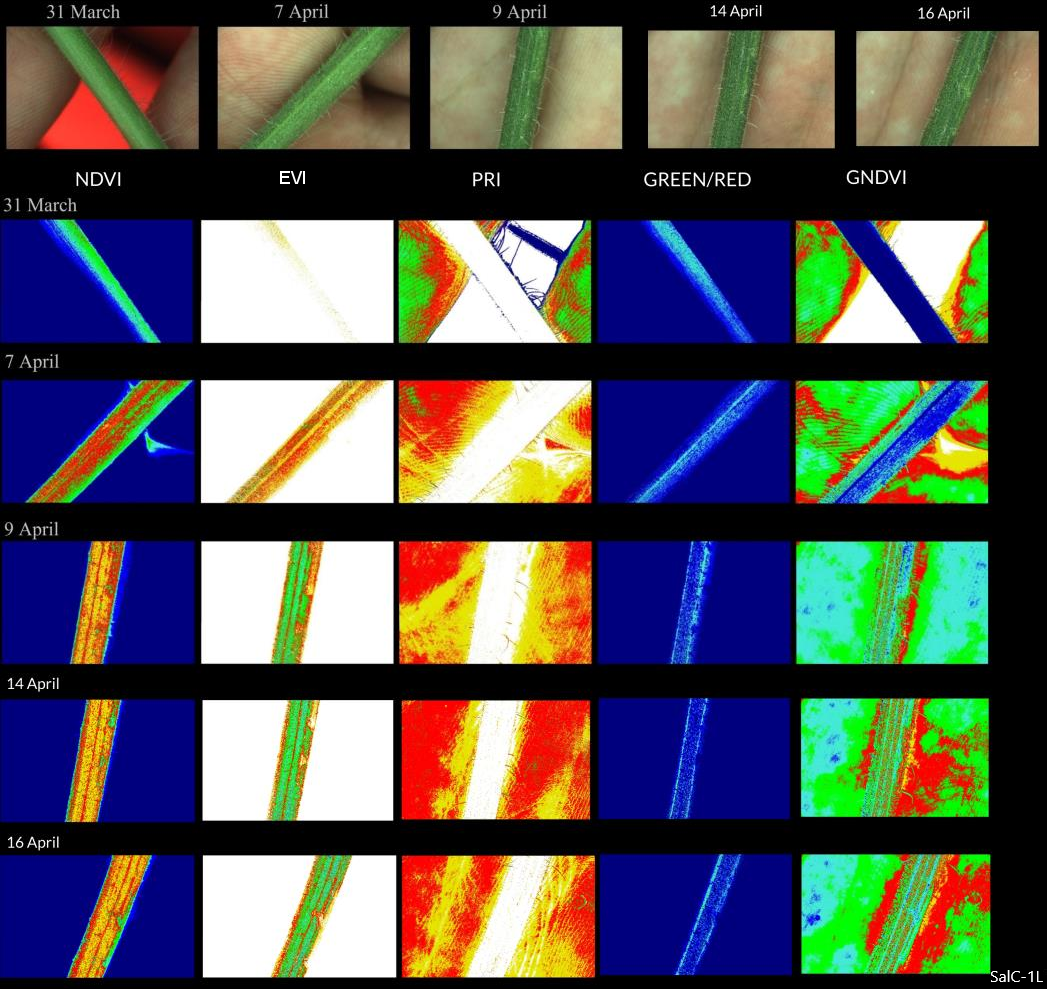
\includegraphics[width=\textwidth,height=0.5\textheight]{Figures/SalC1L.png}
                      \end{subfigure}
                      \qquad
                      \begin{subfigure}[b]{0.72\textwidth}
                        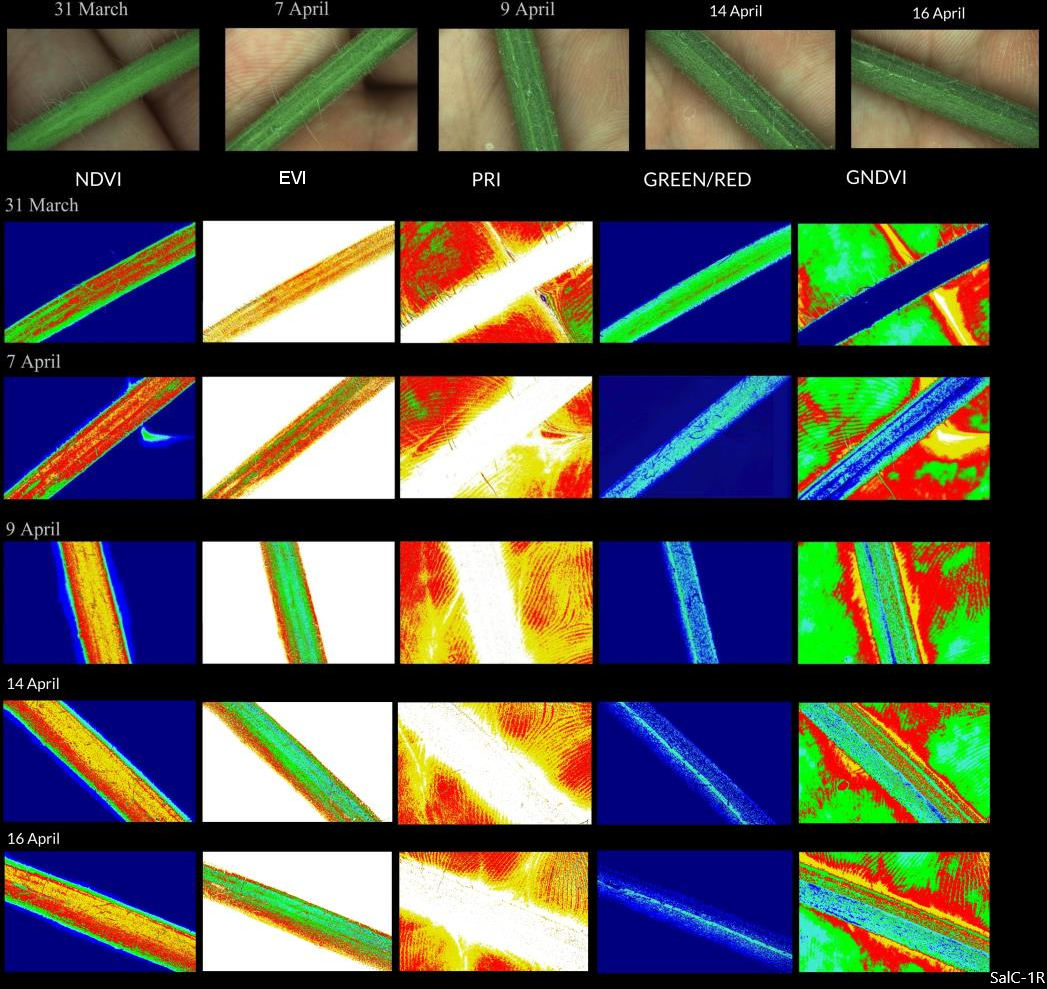
\includegraphics[width=\textwidth,height=0.5\textheight]{Figures/SalC1R.png}
                      \end{subfigure}
                      \caption{SalC1}
                      \label{fig:example}
                    \end{figure}
                    \vspace*{2\baselineskip}
                    
                    \begin{itemize}
                       \item NDVI index changed rapidly from 7th of April to 9th of April, indicating an increase in chlorophyll.
                       \item EVI has a worth mentioning decrease between 7th-9th of April and then it stabilizes.
                       \item GNDVI index shows an increase in water and nitrogen uptake into the plant. Major difference can be observed from 7th to 9th of April.
                       \item PRI index indicates, a good overall health state of the plant.
                       \item As we can observe in the above figures there an no crucial differences between different leaves of this plant.
                    \end{itemize}
                    \newpage
                    \vspace*{-3.8\baselineskip}
                    \hrule
                    \vspace*{3\baselineskip}
                    
                    \begin{figure}[h]
                        \centering
                        \subfloat{{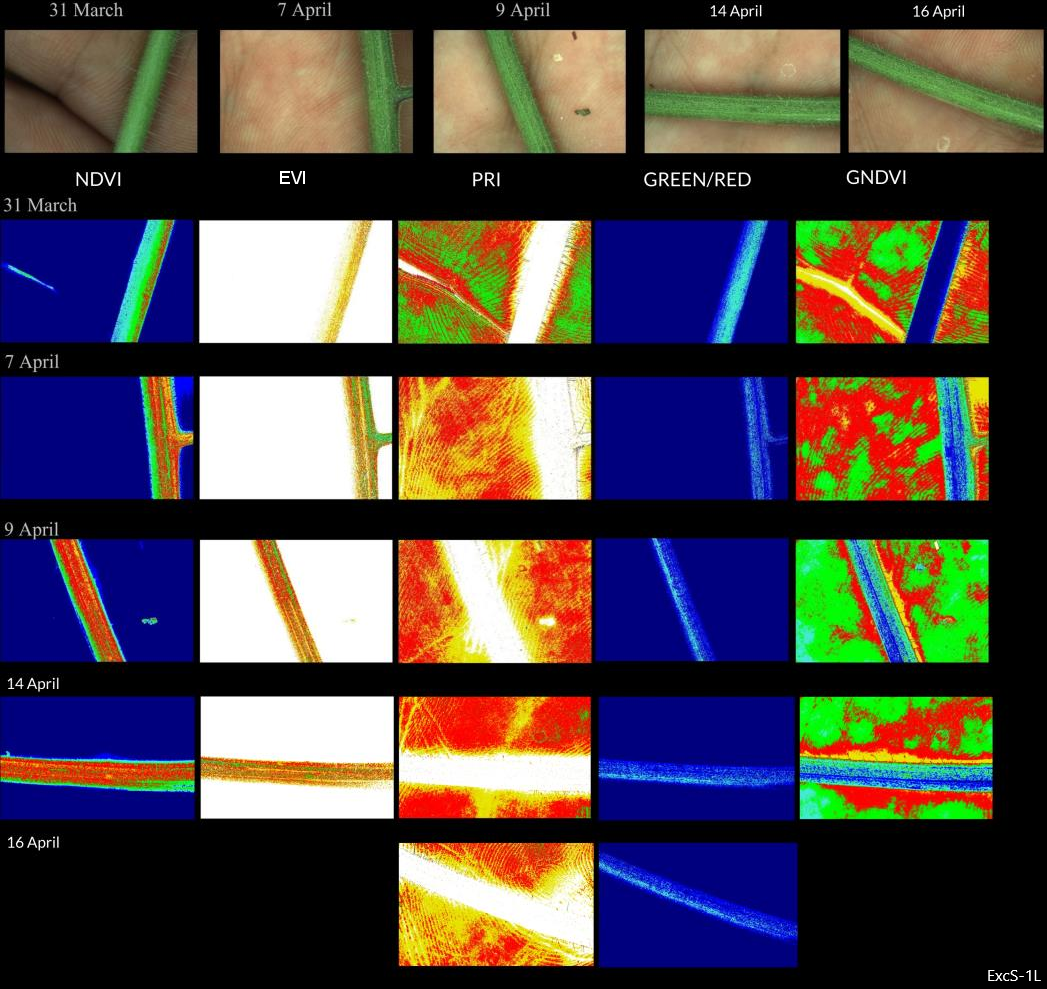
\includegraphics[width=0.72\textwidth,height=0.5\textheight]{Figures/Exc1L.png} }}
                        \qquad
                        \subfloat{{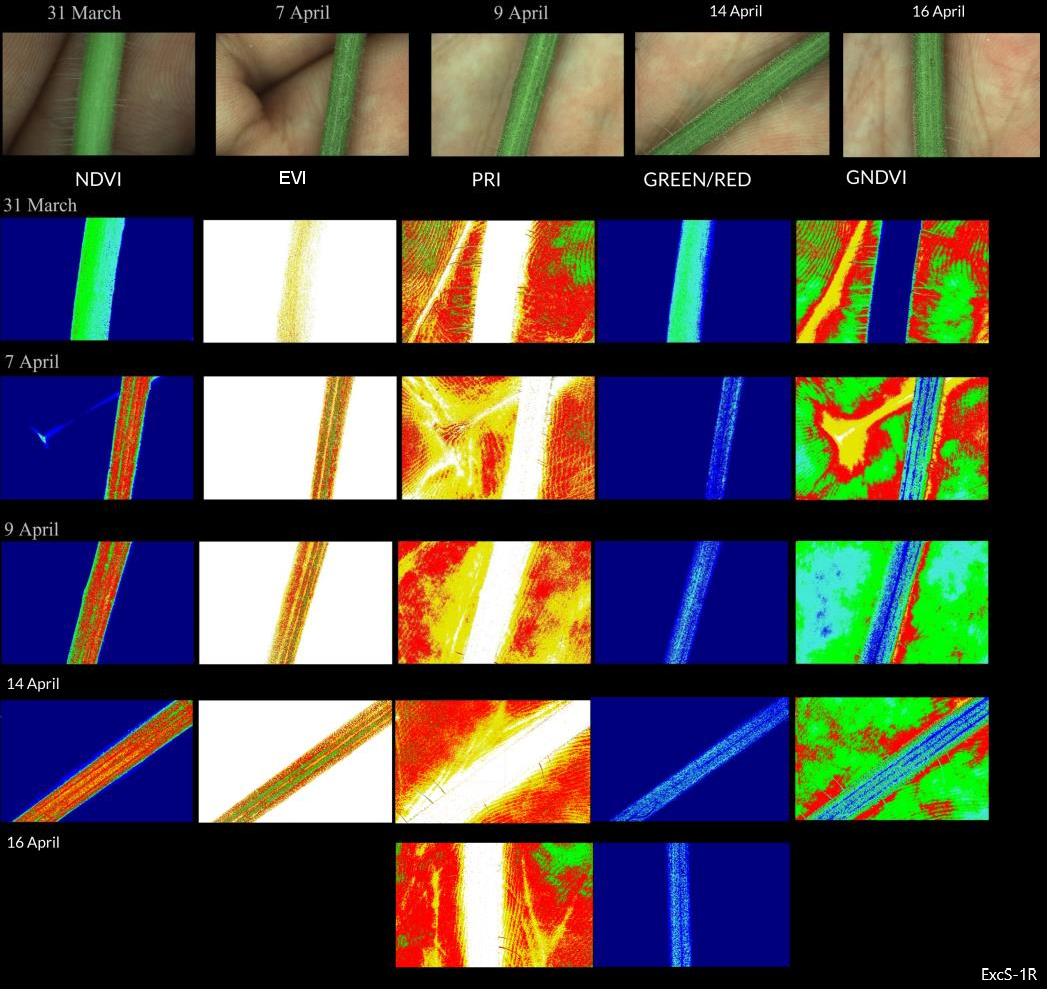
\includegraphics[width=0.72\textwidth,height=0.5\textheight]{Figures/Exc1R.png} }}
                        \caption{ExcS1}%
                        \label{fig:example}
                    \end{figure}
                    \vspace*{2\baselineskip}
                    
                    \begin{itemize}
                       \item  Compared to the equivalent aforementioned plant, we can observe an alteration in NDVI index. Specifically due to salinity, chlorophyll concentration of the plant has been dropped. This causes a decrease in photosynthetic rate since chlorophyll is the primary pigment used in photosynthesis.
                       \item  Photochemical reflectance index (PRI) indicates the efficiency in which carotenoid pigments can harvest light for photosynthesis .However there is no obvious difference as it should be since PRI index could be used as a reliable water-stress index.
                        \item  GRVI (Green Red Vegetation Index) , shows a decrease in chlorophyll from the first days of our experiment. For that reason it is a great index to assess the levels of chlorophyll and thus the light-levels and water-nutrients parameters of photosynthetic rate.
                        \item  As we expected GNDVI decreases in comparison with SalC1 and reaches a certain level. Water and nitrogen uptake declines with the presence of salinity. That verifies GRVI as nitrogen is a vital component of chlorophyll.

                    \end{itemize}
                    \newpage
                    \vspace*{-3.8\baselineskip}
                    \hrule
                    \vspace*{3\baselineskip}
                    
                    \begin{figure}[h]
                        \centering
                        \subfloat{{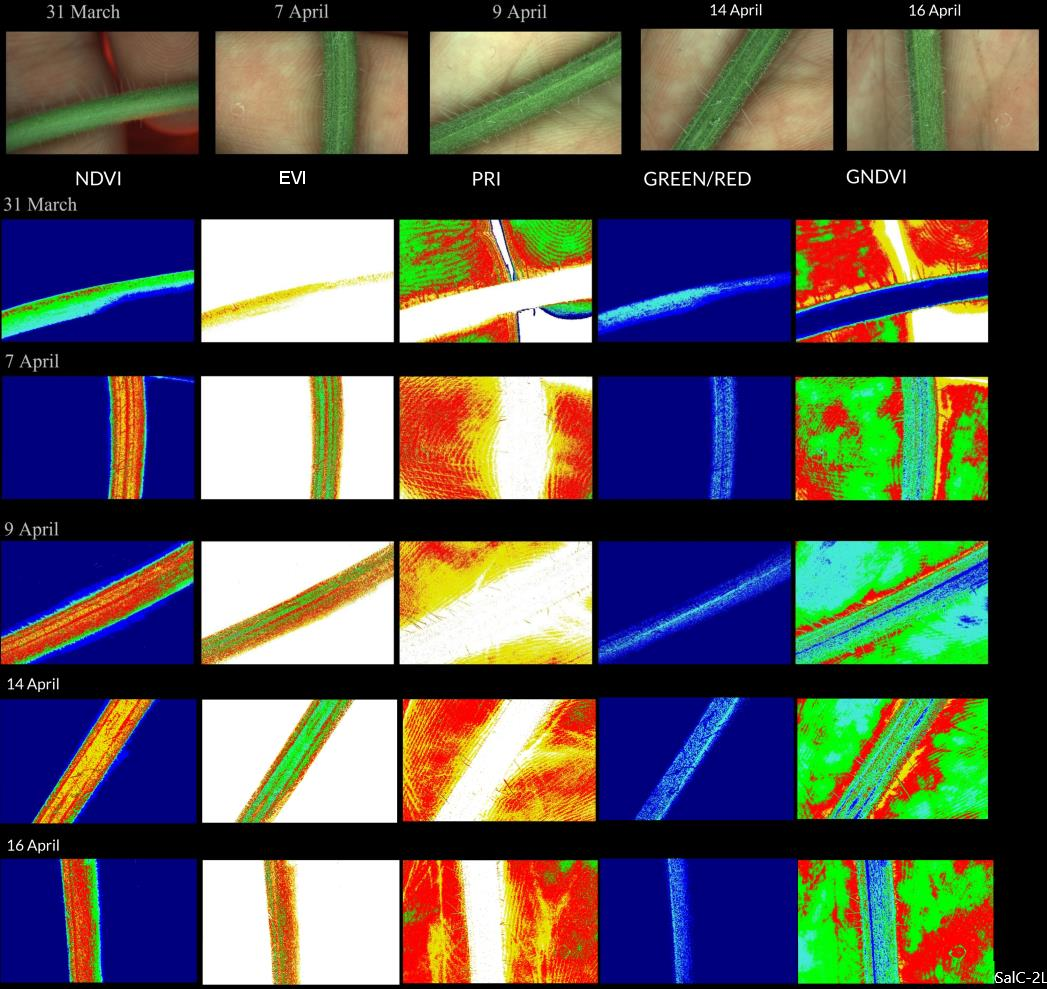
\includegraphics[width=0.72\textwidth,height=0.5\textheight]{Figures/SalC2L.png}}}
                        \qquad
                        \subfloat{{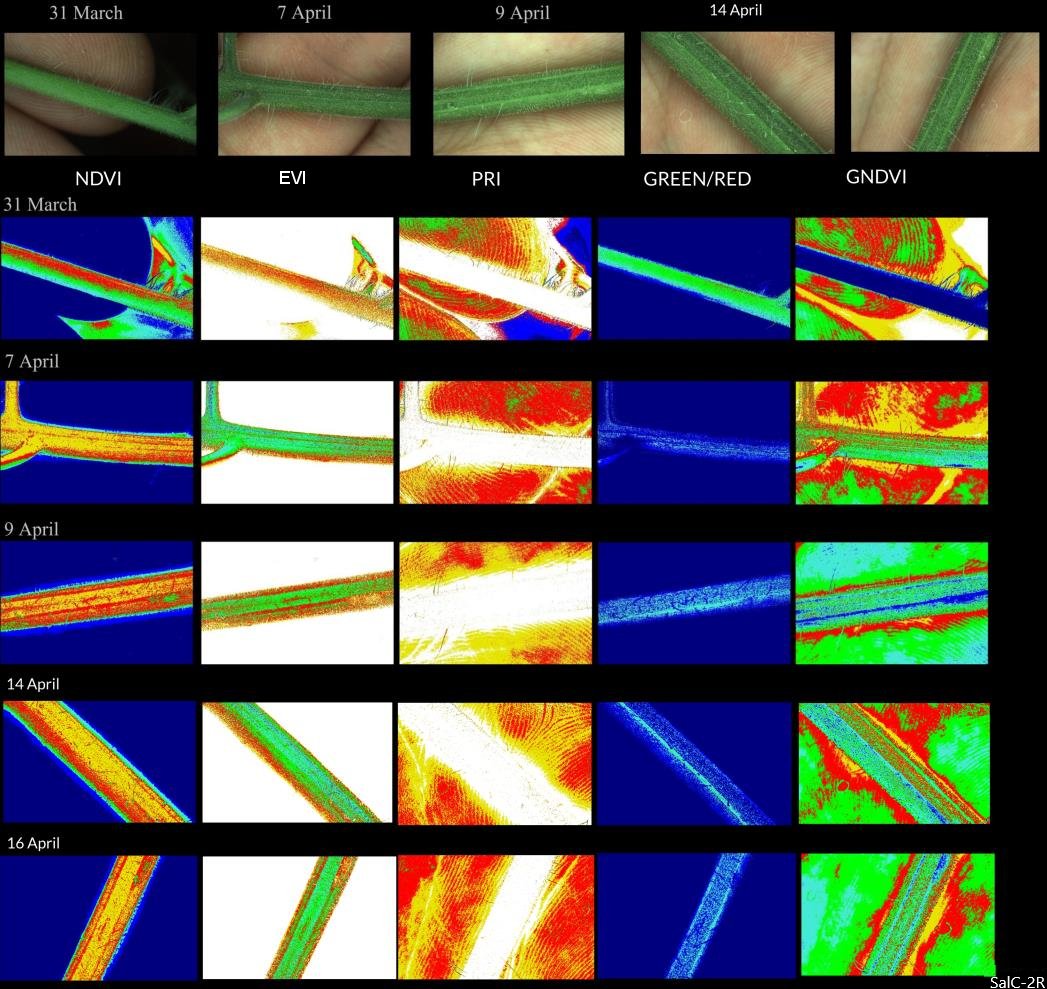
\includegraphics[width=0.72\textwidth,height=0.5\textheight]{Figures/SalC2R.png}}}
                        \caption{SalC2}%
                        \label{fig:example}
                    \end{figure}
                    \vspace*{2\baselineskip}
                    
                    \begin{itemize}
                       \item In comparison with SalC1, it is worth mentioning that there is a difference in NDVI, EVI & GREEN/RED index between different leaves of the same plant (31th of March, 16th of April). This could be a useful information since it indicates that vegetation indices can differ from leaf to leaf.
                       \item In broad terms both SalC1 and SalC2 have no major differences except the one that I have prementioned.
                    \end{itemize}
                    \newpage
                    \vspace*{-3.8\baselineskip}
                    \hrule
                    \vspace*{3\baselineskip}
                    
                    \begin{figure}[h]
                        \centering
                        \subfloat{{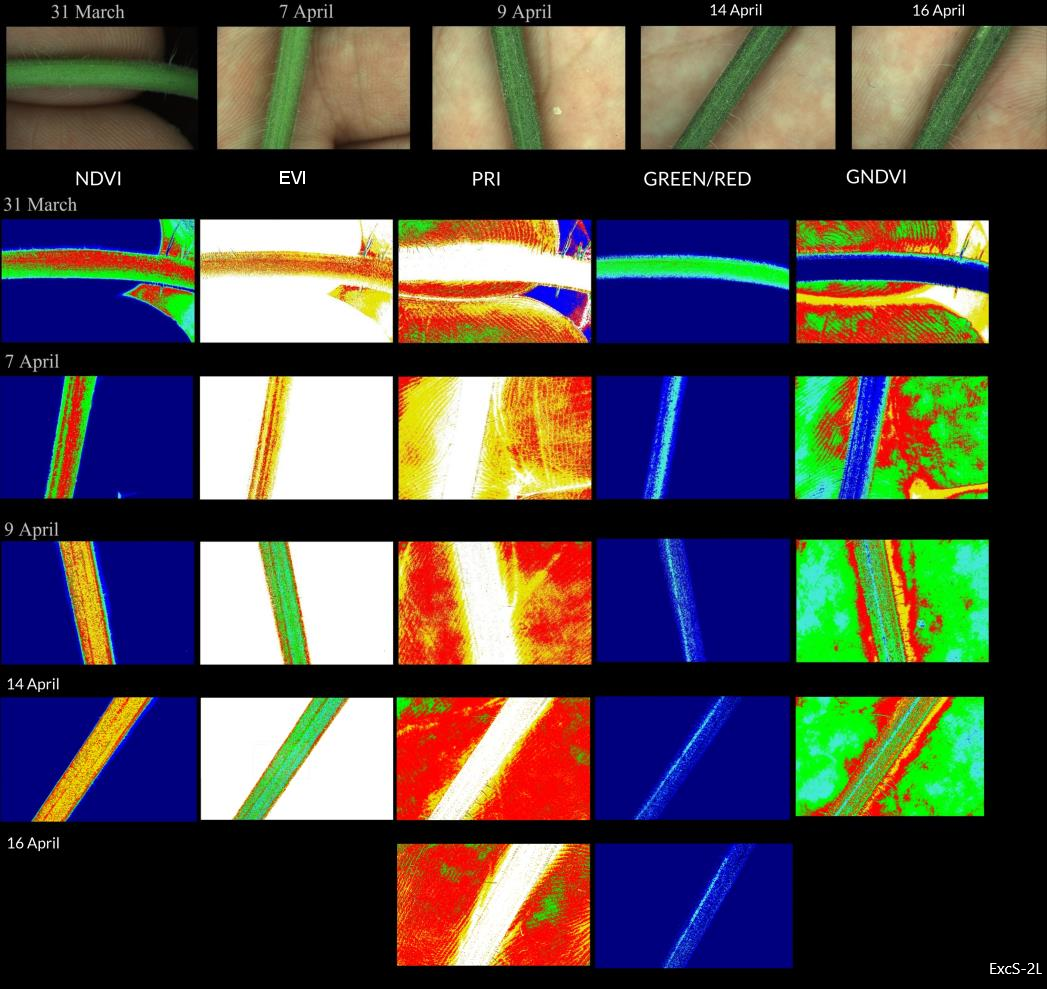
\includegraphics[width=0.72\textwidth,height=0.5\textheight]{Figures/Exc2L.png}}}
                        \qquad
                        \subfloat{{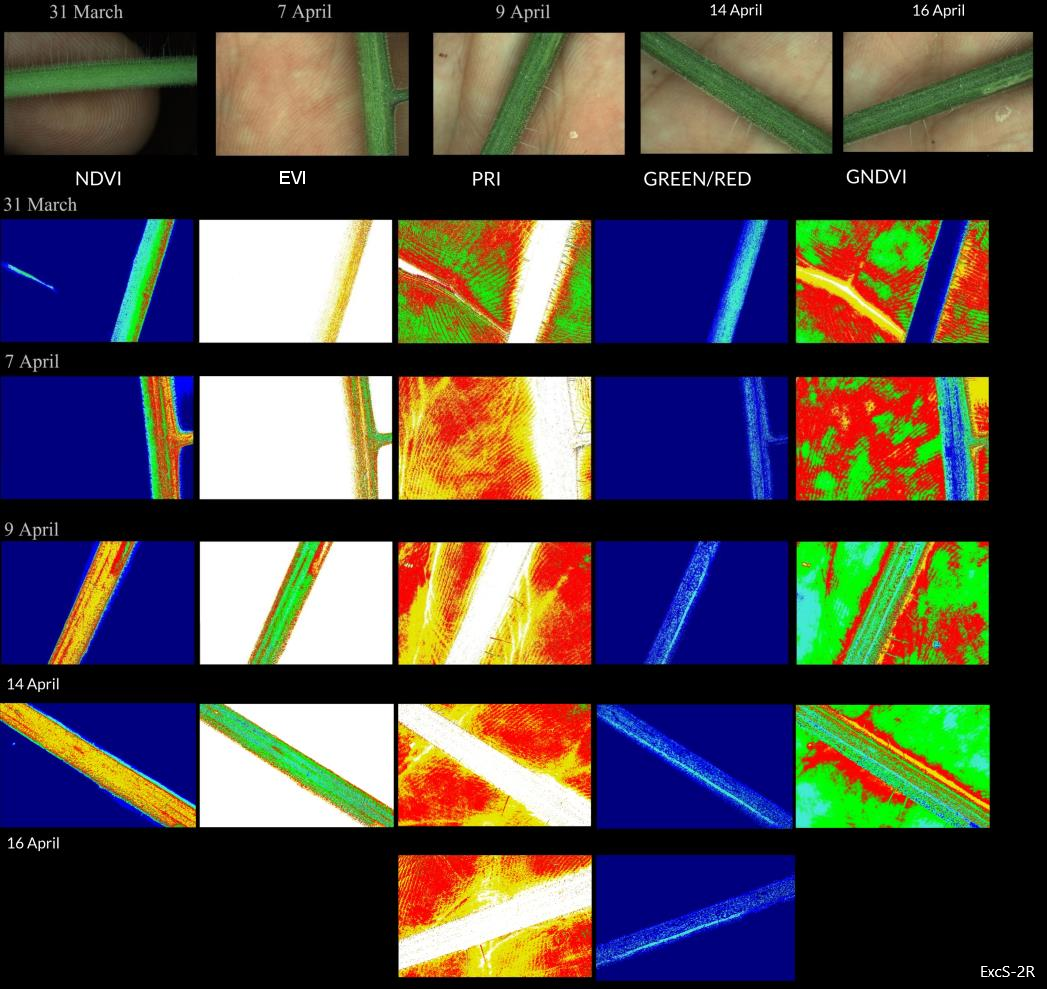
\includegraphics[width=0.72\textwidth,height=0.5\textheight]{Figures/Exc2R.png}}}
                        \caption{ExcS2}%
                        \label{fig:example}
                    \end{figure}
                    \vspace*{2\baselineskip}
                    
                    \begin{itemize}
                       \item Although ExcS2 is exposed to salinity , NDVI & GNDVI show a greater value than ExcS1 and hence high concentration of chlorophyll (almost the same levels of concentration with ExcS2) and nitrogen.
                       \item Vegetation indices in ExcS2 plant have high values, identical with ExcS2 plants. This is not indicative of the presence of salinity, as we would expect for a "salinity" plant. However ExcS2 is the only "salinity" plant which shows such great values.
                    \end{itemize}
                    \newpage
                    \vspace*{-3.8\baselineskip}
                    \hrule
                    \vspace*{3\baselineskip}
                    
                    \begin{figure}[h]
                        \centering
                        \subfloat{{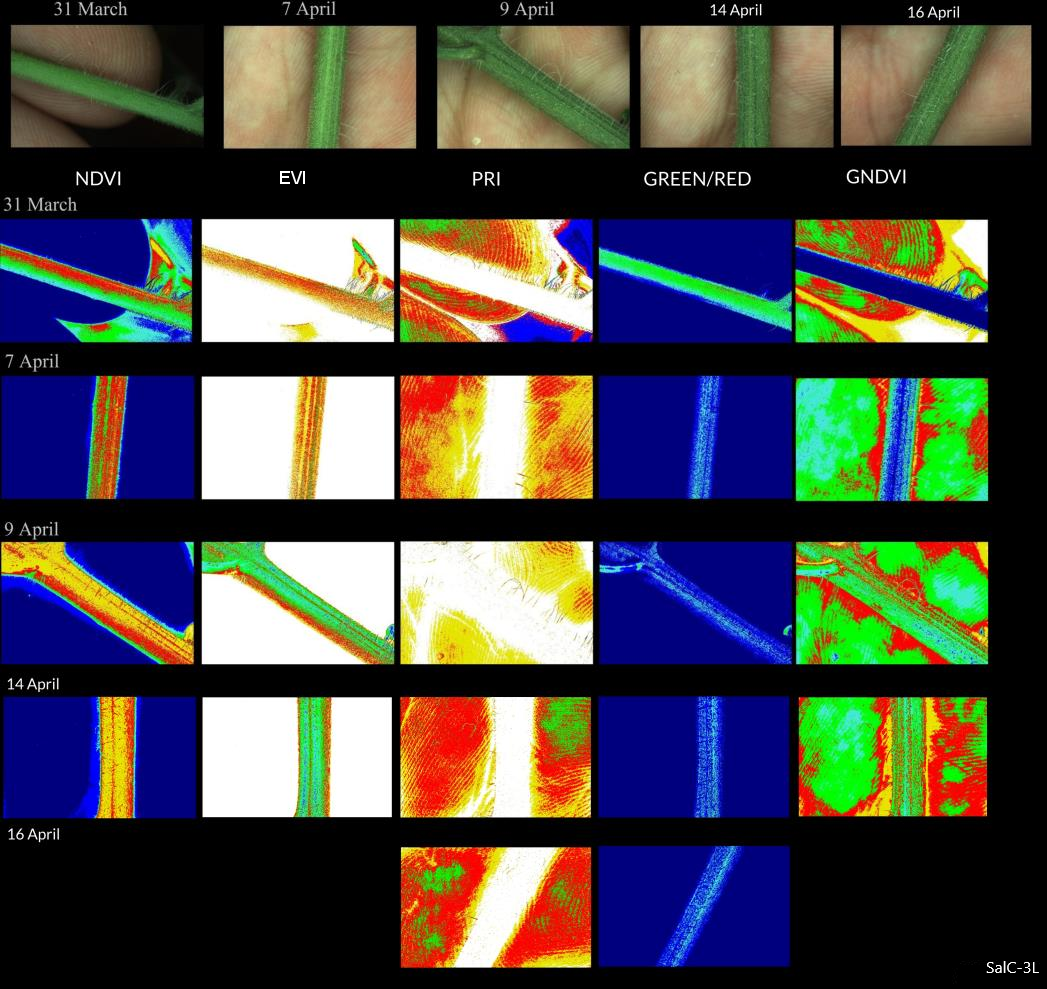
\includegraphics[width=0.72\textwidth,height=0.5\textheight]{Figures/SalC3L.png}}}
                        \qquad
                        \subfloat{{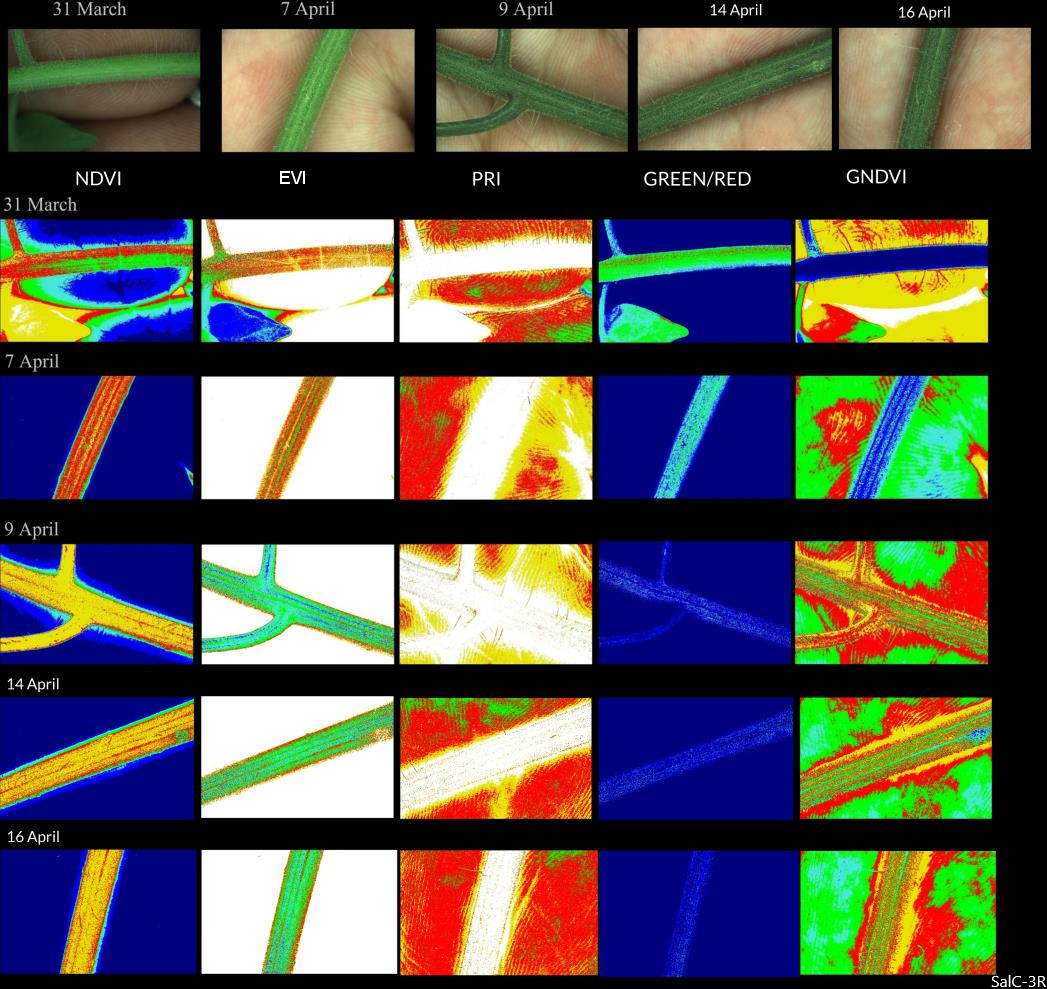
\includegraphics[width=0.72\textwidth,height=0.5\textheight]{Figures/SalC3R.png}}}
                        \caption{SalC3}%
                        \label{fig:example}
                    \end{figure}
                    \vspace*{2\baselineskip}
                    
                    \begin{itemize}
                       \item SalC3 indices comport with the ones of SalC1 & SalC2.
                      % \item GRVI levels however are significantly lower in SalC3 in comparison with the afore mentioned plants, something that does not occur in SalC4.

                    \end{itemize}
                    \newpage
                    \vspace*{-3.8\baselineskip}
                    \hrule
                    \vspace*{3\baselineskip}
                    
                    \begin{figure}[h]
                        \centering
                        \subfloat{{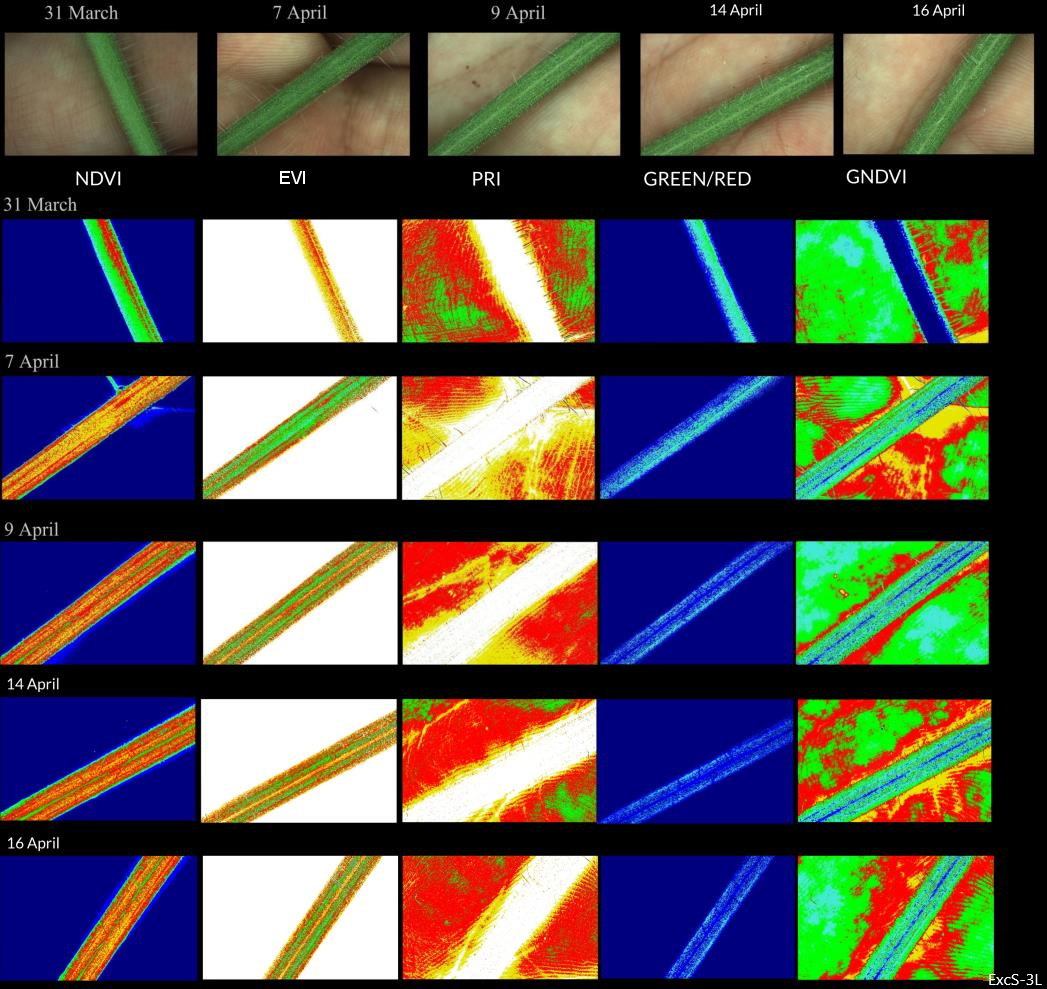
\includegraphics[width=0.72\textwidth,height=0.5\textheight]{Figures/Exc3L.png} }}
                        \qquad
                        \subfloat{{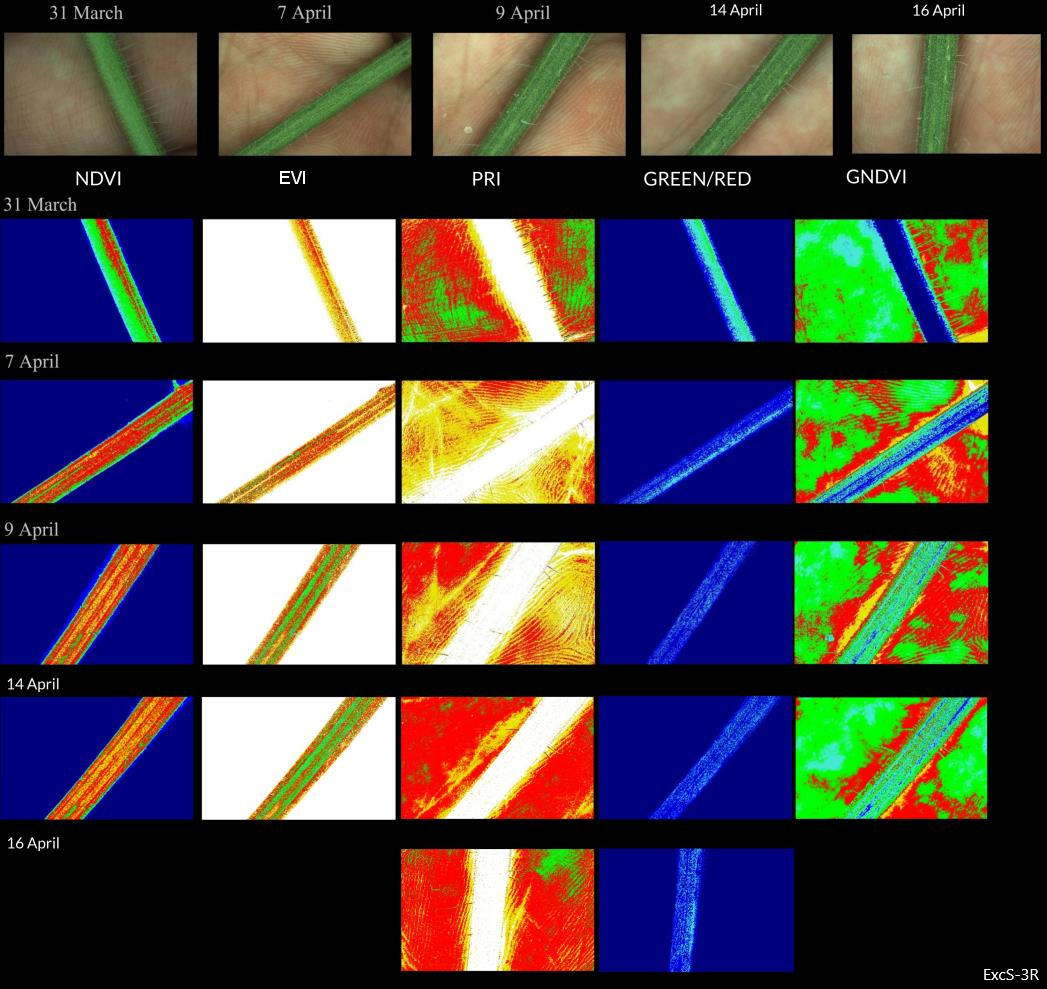
\includegraphics[width=0.72\textwidth,height=0.5\textheight]{Figures/ExcS3R.png} }}
                        \caption{ExcS3}%
                        \label{fig:example}
                    \end{figure}
                    \vspace*{2\baselineskip}
                    
                    \begin{itemize}
                       \item ExcS3 shows the same decreases in response with ExcS1 & ExcS2 (except from the increase of NDVI & GNDVI of ExcS2)
                    \end{itemize}
                    \newpage
                    \vspace*{-3.8\baselineskip}
                    \hrule
                    \vspace*{3\baselineskip}
                    
                    \begin{figure}[h]
                        \centering
                        \subfloat{{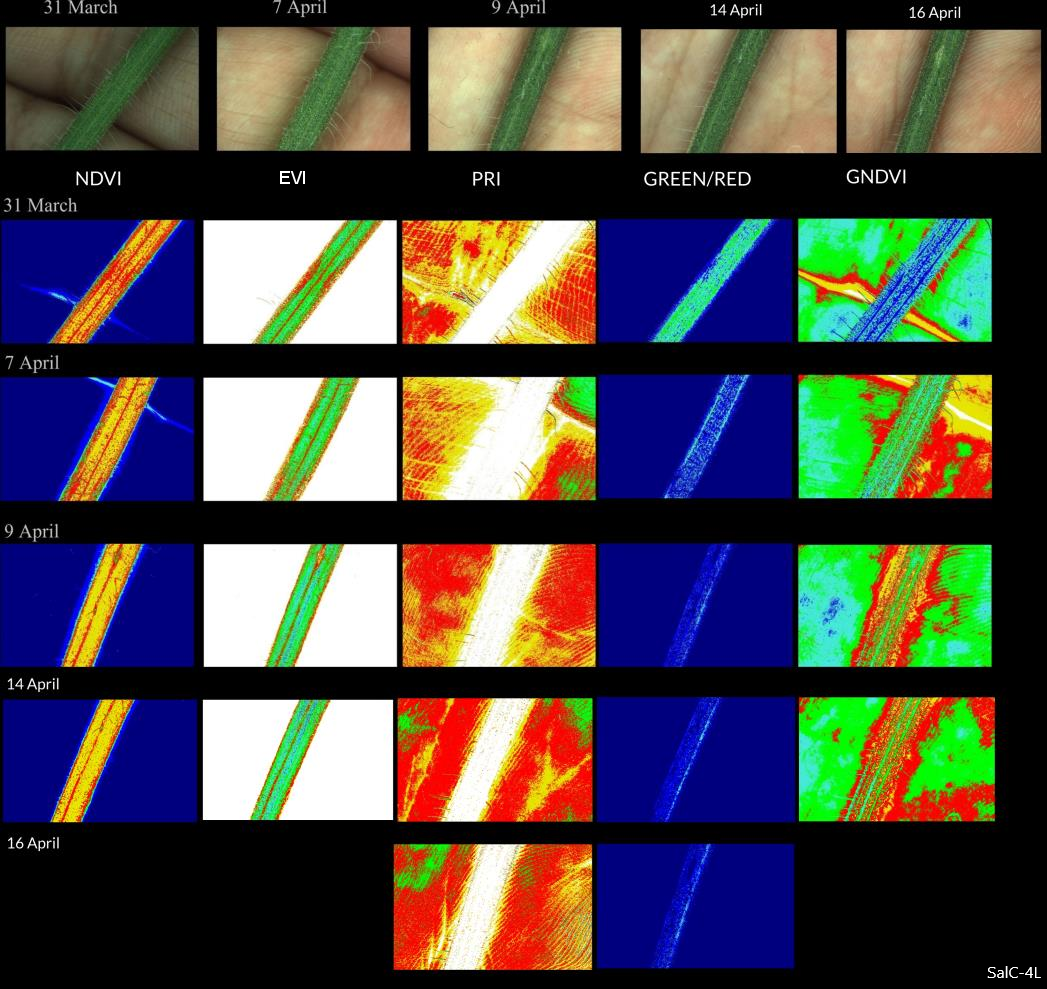
\includegraphics[width=0.72\textwidth,height=0.5\textheight]{Figures/SalC4L.png} }}
                        \qquad
                        \subfloat{{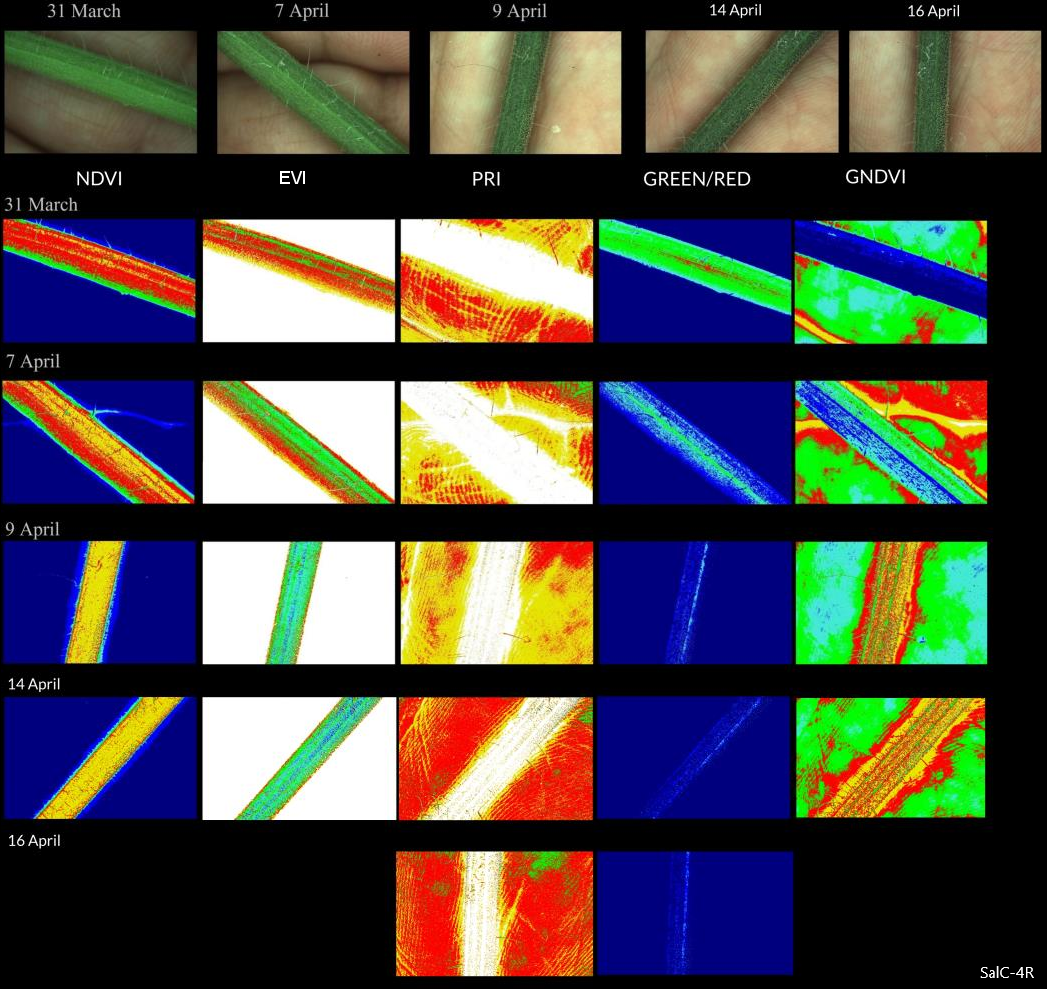
\includegraphics[width=0.72\textwidth,height=0.5\textheight]{Figures/SalC4R.png} }}
                        \caption{SalC4W}%
                        \label{fig:example}
                    \end{figure}
                    \vspace*{2\baselineskip}
                    
                    \begin{itemize}
                       \item GNDVI values show water and nitrogen uptake , thus W (SalC-iW, ExcS-iW)  plants should have lower values than Exc & SalC 1-3 plants cause they were over exposed to water. Every sample was planted in the same type of soil (same nitrogen concentration) and the only difference concerning GNDVI was the amount of water provided to each plant. This is the reason why we can not conclude about water intake using GNDVI.

                    \end{itemize}
                    \newpage
                    \vspace*{-3.8\baselineskip}
                    \hrule
                    \vspace*{3\baselineskip}
                    
                    \begin{figure}[h]
                        \centering
                        \subfloat{{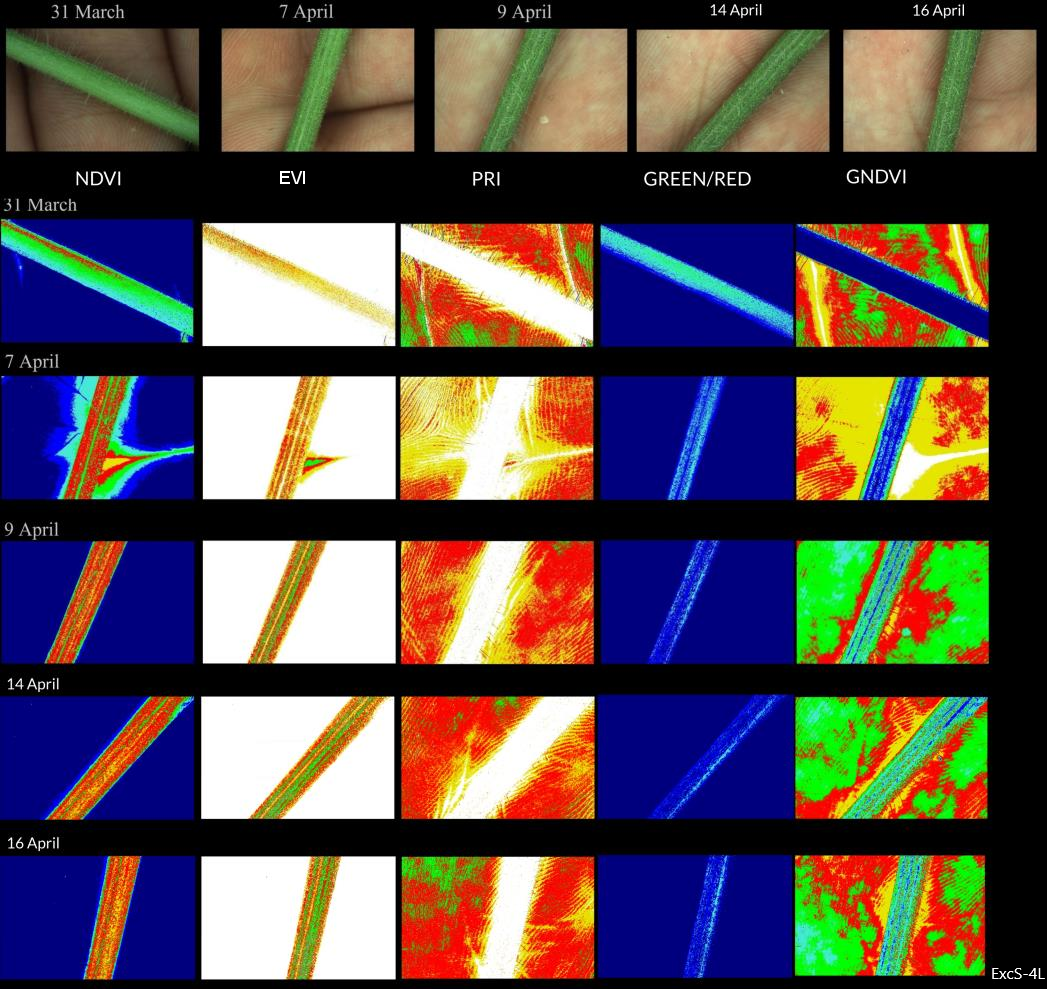
\includegraphics[width=0.72\textwidth,height=0.5\textheight]{Figures/Exc4L.png} }}
                        \qquad
                        \subfloat{{\includegraphics[width=0.72\textwidth,height=0.5\textheight]{Figures/Exc4R.png} }}
                        \caption{ExcS4W}%
                        \label{fig:example}
                    \end{figure}
                    \vspace*{2\baselineskip}
                    
                    \begin{itemize}
                       \item Apart from W plants, NDVI & GNDVI indices have lower values due to salinity.
                    \end{itemize}
                    \newpage
                    \vspace*{-3.8\baselineskip}
                    \hrule
                    \vspace*{3\baselineskip}
                    
                    \begin{figure}[h]
                        \centering
                        \subfloat{{\includegraphics[width=0.72\textwidth,height=0.5\textheight]{Figures/SalC5L.jpg} }}
                        \qquad
                        \subfloat{{\includegraphics[width=0.72\textwidth,height=0.5\textheight]{Figures/SalC5R.jpg} }}
                        \caption{SalC5W}%
                        \label{fig:example}
                    \end{figure}
                    \vspace*{2\baselineskip}
                    
                    \begin{itemize}
                       \item  NDVI index has lower values in comparison with the previous "Control" plants and instead of increasing through time like the other plants , it decreases.
                    \end{itemize}
                    \newpage
                    \vspace*{-3.8\baselineskip}
                    \hrule
                    \vspace*{3\baselineskip}
                    
                    \begin{figure}[h]
                        \centering
                        \subfloat{{\includegraphics[width=0.72\textwidth,height=0.5\textheight]{Figures/Exc5L.png}}}
                        \qquad
                        \subfloat{{\includegraphics[width=0.72\textwidth,height=0.5\textheight]{Figures/Exc5R.png}}}
                        \caption{ExcS5W}%
                        \label{fig:example}
                    \end{figure}
                    \vspace*{2\baselineskip}
                    
                    \begin{itemize}
                       \item  SalC4W and ExcS4W have obvious dissimilarities in their indices. SalC5W and ExcS5W have no crucial differences between them.
                    \end{itemize}
                    
                    \newpage
                    \vspace*{-3.8\baselineskip}
                    \hrule
                    \vspace*{1\baselineskip}
                    
                    \subsection{Results}
                    
                    \begin{table}[h]
                      \centering
                      \caption{Result Table}
                      \vspace*{2\baselineskip}
                      \label{tab:result-table}
                      \renewcommand{\arraystretch}{2.5} % adjust cell height
                      \resizebox{\textwidth}{!}{
                      \begin{tabular}{|p{2cm}|p{4cm}|p{5cm}|p{4cm}|p{4cm}|p{4cm}|}
                        \hline
                        \textbf{} & \centering \textbf{CHLOROPHYLL CONCENTRATION} & \centering  \textbf{NITROGEN LEVELS} & \centering \textbf{SALINITY} & \centering \textbf{PHOTOSYNTHETIC RATE} & \hspace{0.2cm} \textbf{WATER UPTAKE} \\ 
                        \hline
                        \centering \vspace{0.4cm}NDVI & \cellcolor{green!30}  & \cellcolor{green!30}  & \cellcolor{green!30} &         \cellcolor{green!30}  & \cellcolor{red!30}
                        \\
                        \hline
                        
                        \centering \vspace*{1\baselineskip}PRI & \cellcolor{red!30}  & \cellcolor{red!30}  & \cellcolor{red!30} & \cellcolor{red!30}   & \cellcolor{red!30} 
                        \\
                        \hline
                        
                        \centering \vspace{0.1cm}GRVI & \cellcolor{green!30} & \cellcolor{green!30}  &\centering \vspace{-0.4cm} not very informative & \cellcolor{green!30}    & \cellcolor{red!30} \\
                        \hline
                        
                        \centering \vspace*{1\baselineskip}GNDVI & \cellcolor{green!30}  & \cellcolor{green!30}  & \cellcolor{green!30}  &       \cellcolor{green!30}& \cellcolor{red!30}                               \\
                            \hline
                       \end{tabular}}
                    \end{table}
                    \vspace*{2\baselineskip}
                    
                    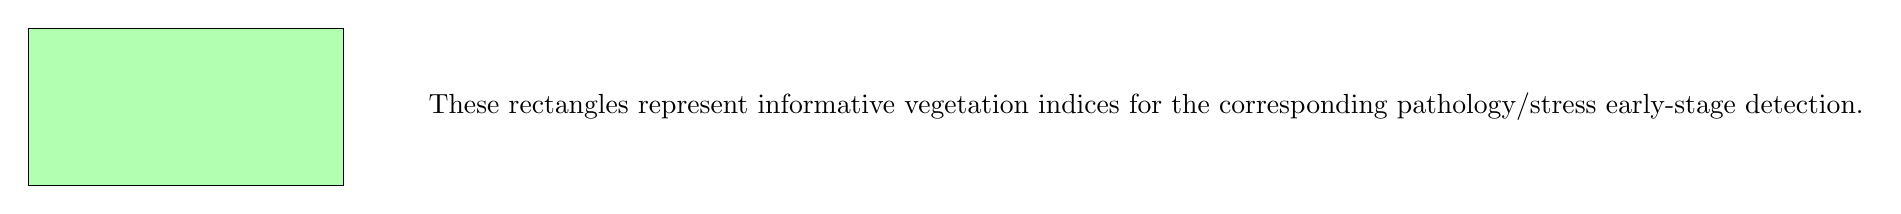
\begin{tikzpicture}
                        \filldraw[green!30, draw=black] (0,0) rectangle (4,2);
                        \node[right] at (4,1) {\hspace{2\baselineskip} These rectangles represent informative vegetation indices for the corresponding pathology/stress early-stage detection.};
                    \end{tikzpicture}
                    \vspace{2\baselineskip}

                    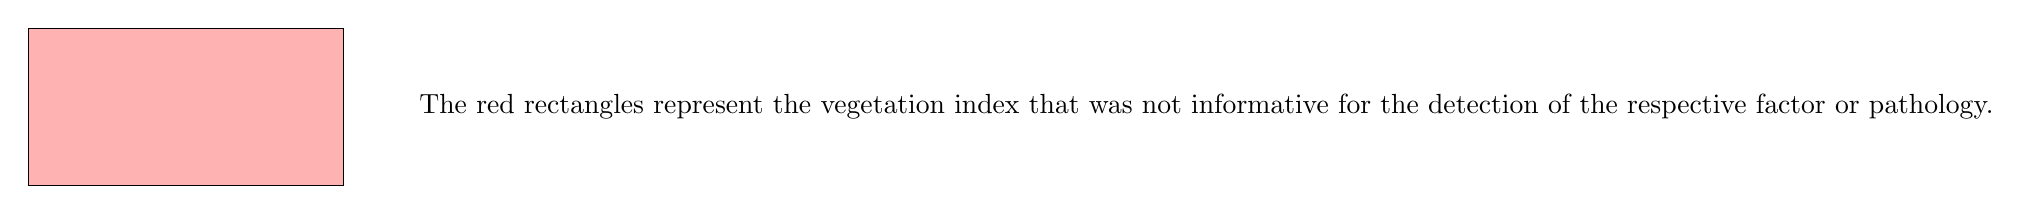
\begin{tikzpicture}
                        \filldraw[red!30, draw=black] (0,0) rectangle (4,2);
                        \node[right] at (4,1) {\hspace{2\baselineskip}The red rectangles represent the vegetation index that was not informative for the detection of the respective factor or pathology.};
                    \end{tikzpicture}
                    
               \end{landscape}}
                    The table presented above provides a summary of the results obtained from using four vegetation indices to detect the presence of different stress factors affecting plant growth. The cells of the table are color-coded to indicate the informative value of each vegetation index for a particular stress factor. In this context, red cells indicate that the vegetation index did not provide any detectable results in identifying the stress factor, while green cells show that the index was informative about the specific stress factor.\par
                    \vspace*{1\baselineskip}
                    
                    It is important to note that the indices that produced green cells in the table were able to detect the stress factor in question with a certain level of accuracy. For example the Normalized Difference Vegetation Index (NDVI) and Green Normalized Difference Vegetation Index (GNDVI) indices were mostly informative in identifying the majority of stress factors. On the other hand, indices that produced more red cells such as the Green-Red Vegetation Index(GRVI) and Photochemical Reflectance Index (PRI) were part useful or not useful at all in detecting any stress factors that we included in our experiment accordingly. In the following paragraphs, we will delve deeper into the findings of our study regarding the informativeness of each row, column and cell of the table.\par
                    \vspace*{1\baselineskip}
                    
                    \subsubsection{Pathologies}
                    
                     As the results were analyzed, we found that each vegetation index in the table provided some level of information on various plant pathologies and stress factors with the exception of PRI index. However, no measurement can provide a complete picture of plant growth and health, and it is crucial to consider multiple factors when assessing plant health. By combining multiple measurements and considering various factors such as nutrient availability, water availability and lighting, we could better understand plant health and develop more effective strategies for improving crop yield and sustainability.\par
                    \vspace*{1\baselineskip}

                    Overall, our study has provided important insights into real-time in situ detection and mapping of plant pathologies. By utilizing hyperspectral imaging combined with in situ mapping via Classification, we can detect early signs of stress or disease in plants and monitor their growth and health. These findings have significant implications for agriculturalists and plant pathologists, as they can develop spectral libraries for different pathologies and stress factors and automate plant monitoring. Our work contributes to the ongoing efforts to develop more efficient and sustainable methods for crop production,through in situ and non destructive crop monitoring which is critical to ensuring food security for the growing global population.\par
                    \vspace*{1\baselineskip}
                    
                    \textbf{CHLOROPHYLL CONCENTRATION} was detectable for the vast majority of the V.I. used. Measuring chlorophyll concentration can be useful in determining plant health and detecting early signs of stress or disease. This is because chlorophyll is essential for photosynthesis, and any decrease in concentration can indicate a decrease in plant health. However, chlorophyll concentration alone may not provide a complete picture of plant health, as other factors such as nutrient deficiencies, disease, and environmental stressors can also impact plant growth and health.\par
                    \vspace*{1\baselineskip}
                    
                    \textbf{NITROGEN LEVELS} changes were mostly visible even from the early stages of plant growth as chlorophyll concentration. Nitrogen is a critical nutrient for plant growth and is essential for protein synthesis, chlorophyll production, and overall plant health. Measuring nitrogen levels can provide valuable information on plant nutrition status and help identify potential deficiencies. However, nitrogen levels alone may not be sufficient to fully understand plant health as we have already prementioned, as other factors such as water availability, soil pH, and temperature can also affect plant growth and health.\par
                    \vspace*{1\baselineskip}
                    
                    \textbf{SALINITY LEVELS} , were difficult to identify for the majority of our V.I.. Salinity is a stress factor for plants, and measuring salinity levels can provide valuable information on the degree of salt stress in the soil. However, salinity alone may not be a reliable indicator of plant health, as plants can adapt to salt stress through various mechanisms such as osmotic adjustment and ion exclusion which have to be taken into consideration. Therefore, while salinity measurements can be useful in identifying areas of high salt stress, other factors such as nutrient availability and water availability should also be considered to fully understand the impact of salinity on plant health.\par
                    \vspace*{1\baselineskip}
                    
                    \textbf{PHOTOSYNTHETIC RATE} is highly informative in assessing plant health and was highly detectable. Photosynthesis is the process by which plants convert sunlight into energy, and measuring photosynthetic rate can provide valuable information on plant growth and health as we described in chapter 2. A higher photosynthetic rate indicates that the plant is producing more energy and is likely healthier than a plant with a lower photosynthetic rate. Therefore, measuring photosynthetic rate is crucial in understanding the overall health of the plant and detecting early signs of stress or disease.\par
                    \vspace*{1\baselineskip}
                    
                    Finally, \textbf{WATER UPTAKE} was not traceable by any of the V.I. used. Water is an essential nutrient for plant growth, and measuring water uptake can provide valuable information on plant water use efficiency and drought tolerance. A plant with a high water uptake rate is likely more efficient at using water and more tolerant to drought stress than a plant with a low water uptake rate. Therefore, measuring water uptake is crucial in understanding plant health and drought tolerance.\par
                    \vspace*{1\baselineskip}
                    
                    
                    The results presented highlight the importance of carefully selecting the appropriate vegetation index for the stress factor being studied. If an index is not informative for a particular stress factor, it may be necessary to explore other indices or more complex methods to detect the stress or the pathology. This information can help guide future research efforts and inform agricultural practices aimed at improving plant growth in challenging environments.\par
                    \vspace*{1\baselineskip}
                    
                    In conclusion, the table provided valuable information on various vegetation indices and plant stress factors. Each cell had its own level of informativeness in assessing plant health, with some cells providing more valuable information than others. However, it is important to consider multiple factors when assessing plant health, as no single measurement can provide a complete picture of plant growth and health. By combining multiple measurements and considering various factors, researchers can better understand plant health and develop more effective strategies for improving crop yield and sustainability.\par
                    
                    \newpage
                    
                    \subsubsection{Vegetation Indices}
                    
                    NDVI is an effective vegetation index for assessing the chlorophyll concentration, nitrogen levels, salinity, and photosynthetic rate of plants. However, it is not informative for assessing water uptake. This is because NDVI is primarily sensitive to the amount of chlorophyll in the leaves, which is directly related to the amount of light absorbed by the plants for photosynthesis. While water is also necessary for photosynthesis, NDVI does not directly measure the amount of water that plants take up, making it less useful for evaluating water stress in plants.\par
                    \vspace*{1\baselineskip}

                    PRI, on the other hand, is not a particularly informative vegetation index for any of the five plant health parameters considered here. It is primarily sensitive to changes in the carotenoid pigments in leaves, which can be affected by stressors such as drought, but its relationship to plant health is not as straightforward as the other indices. Therefore, it may not be the best choice for assessing the health or stress of plants in most situations.\par
                    \vspace*{1\baselineskip}

                    GRVI is informative for assessing chlorophyll concentration, nitrogen levels, and photosynthetic rate, but it is not particularly useful for assessing salinity or water uptake. This is because it is primarily sensitive to the greenness of the leaves, which is related to chlorophyll concentration, but does not directly measure other parameters that influence plant health. However, its sensitivity to chlorophyll makes it a useful index for assessing the overall health and vigor of plants.\par
                    \vspace*{1\baselineskip}

                    GNDVI is an effective vegetation index for assessing chlorophyll concentration, nitrogen levels, and salinity in plants. Like NDVI, it is sensitive to the amount of chlorophyll in the leaves, which makes it useful for evaluating the health and stress of plants under various conditions. However, it is not particularly informative for assessing water uptake, which limits its usefulness in some situations where water stress is a concern.\par
                    \vspace*{1\baselineskip}

                    Overall, the choice of vegetation index depends on the specific plant health parameter being assessed and the conditions under which the plants are growing. NDVI and GNDVI are good choices for assessing chlorophyll concentration, nitrogen levels, and salinity, while GRVI is useful for evaluating overall plant health and vigor. However, none of these indices are particularly informative for assessing water uptake, so alternative methods may need to be used in those situations.Results from the experiment were not so informative. Although NDVI and GNDVI decreased from the presence of salinity, in one case NDVI and GNDVI were identical in SalC and ExcS plants, which should not occur. Furthermore PRI did not alter through the experiment as it should be as water uptake was reduced and water provided was not the same for every plant.
                    \newpage
                    
                    \subsubsection{Table Clarification}
                    
                            \vspace*{3\baselineskip}
                            \textbf{CHLOROPHYLL CONCENTRATION}\par
                            \vspace*{1\baselineskip}
                            \begin{enumerate}
                                \item  NDVI index changed rapidly from 7th of April to 9th of April, indicating an increase in chlorophyll. This may be due to new growth or increased photosynthesis activity.\par
                                \vspace*{1\baselineskip}
                                
                                \item   Compared to the equivalent aforementioned plant, we can observe an alteration in NDVI index. Specifically due to salinity, chlorophyll concentration of the plant has been dropped. This causes a decrease in photosynthetic rate since chlorophyll is the primary pigment used in photosynthesis. Salinity can cause stress to plants and affect their ability to absorb nutrients and water, leading to a decrease in chlorophyll concentration and photosynthetic rate.\par
                                \vspace*{1\baselineskip}
                                
                                \item   NDVI index shows a gradual increase from the first day of our experiment until it reaches its maximum value on the 13th of April. This gradual increase may be due to the plant's growth and development, as well as an increase in photosynthetic activity and chlorophyll concentration.\par
                                \vspace*{1\baselineskip}
                                
                                \item   NDVI index shows a gradual increase from the 31st of March to the 9th of April, followed by a sudden decrease on the 16th of April. This sudden decrease may be due to environmental stress factors, such as drought, nutrient deficiency, or disease, that negatively affect the plant's photosynthetic activity and chlorophyll concentration.\par
                            \vspace*{1\baselineskip}

                            \end{enumerate}
                           
                            \vspace*{3\baselineskip}
                            \textbf{NITROGEN LEVELS}\par
                            \vspace*{1\baselineskip}
                            
                            \begin{enumerate}
                                \item  EVI has a worth mentioning decrease between 7th-9th of April and then it stabilizes. By bibliography this could be due to environmental changes such as a change in temperature or humidity, or a change in the amount of available nutrients.\par
                                \vspace*{1\baselineskip}
                                \item Photochemical reflectance index (PRI) indicates the efficiency in which carotenoid pigments can harvest light for photosynthesis .However there is no obvious difference as it should be since PRI index could be used as a reliable water-stress index. The lack of difference in PRI index between plants may indicate that they are not experiencing significant water stress, or that other environmental factors are masking the effects of water stress on the PRI index.\par
                                \vspace*{1\baselineskip}
                                \item  EVI GREEN/RED index shows a slight decrease from the 31st of March to the 7th of April, followed by a gradual increase until the end of the experiment. This fluctuation may be due to changes in environmental conditions, such as changes in temperature, humidity, or nutrient availability, as well as the plant's growth and development.\par
                                \vspace*{1\baselineskip}
                                \item EVI GREEN/RED index shows a slight increase from the 31st of March to the 9th of April, followed by a gradual decrease until the end of the experiment. This fluctuation may be due to changes in environmental conditions, such as changes in temperature, humidity, or nutrient availability, as well as the plant's growth and development.\par
                                \vspace*{1\baselineskip}
                            \end{enumerate}

                            \newpage
                            \textbf{SALINITY}
                            \vspace*{1\baselineskip}
                            
                            \begin{enumerate}
                                \item GNDVI index shows an increase in water and nitrogen uptake into the plant. Major difference can be observed from 7th to 9th of April. This increase in water and nitrogen uptake may be due to increased precipitation or irrigation, or due to the plant becoming more mature and able to absorb more nutrients.\par
                                \vspace*{1\baselineskip}

                            
                                \item GRVI (Green Red Vegetation Index), shows a decrease in chlorophyll from the first days of our experiment. For that reason it is a great index to assess the levels of chlorophyll and thus the light-levels and water-nutrients parameters of photosynthetic rate. A decrease in chlorophyll concentration can be an indication of stress or poor environmental conditions, and the GRVI index is able to capture these changes in chlorophyll levels.\par
                                \vspace*{1\baselineskip}

                                \item GNDVI index shows a gradual increase from the first day of our experiment until it reaches its maximum value on the 13th of April. This increase may be due to an increase in water and nutrient uptake as the plant grows and develops, as well as an increase in photosynthetic activity and chlorophyll concentration.\par
                                \vspace*{1\baselineskip}
                            
                                \item GNDVI index shows a gradual increase from the 31st of March to the 9th of April, followed by a sudden decrease on the 16th of April. This sudden decrease may be due to environmental stress factors, such as drought, nutrient deficiency, or disease, that negatively affect the plant's water and nutrient uptake and chlorophyll concentration.\par
                             \vspace*{3\baselineskip}
                            \end{enumerate}
                            
                            \textbf{PHOTOSYNTHETIC RATE}
                            \vspace*{1\baselineskip}

                            \begin{enumerate}
                                \item PRI index indicates, a good overall health state of the plant. This is because the PRI index is closely correlated with photosynthetic efficiency, and a healthy plant will have higher photosynthetic efficiency.\par
                                \vspace*{1\baselineskip}
                            
                                \item As we expected GNDVI decreases in comparison with SalC1 and reaches a certain level. Water and nitrogen uptake declines with the presence of salinity. That verifies GRVI as nitrogen is a vital component of chlorophyll. The decrease in GNDVI index may indicate reduced water and nutrient uptake due to salinity stress, which is also supported by the decrease in chlorophyll concentration (as indicated by the GRVI index).\par
                                \vspace*{1\baselineskip}
                    
                                \item PRI index shows a slight increase from the 31st of March to the 7th of April, followed by a gradual decrease until the end of the experiment. This fluctuation may be due to changes in environmental conditions, such as changes in temperature, humidity, or nutrient availability, as well as the plant's growth and development.Still not informative at all.\par
                                \vspace*{1\baselineskip}
                            
                                \item The PRI index shows a sharp increase from March 15 to March 25, indicating a significant increase in photosynthetic efficiency. This could be due to optimal growing conditions, such as the right balance of sunlight and nutrients, or due to the plant undergoing a growth phase where it requires more energy for photosynthesis.\par
                                \vspace*{1\baselineskip}
                                \end{enumerate}
                            
                            \newpage
                            \textbf{WATER UPTAKE}
                            \vspace*{1\baselineskip}
                            \begin{enumerate}
                                \item As we can observe in the above figures there an no crucial differences between different leaves of this plant. This suggests that the plant is relatively uniform in terms of its health and growth, and that any differences observed in the indices are likely due to environmental factors rather than genetic variability.\par
                                
                                \item  In comparison with SalC1, it is worth mentioning that there is a difference in NDVI, EVI GREEN/RED index between different leaves of the same plant (31th of March, 16th of April). This could be a useful information since it indicates that vegetation indices can differ from leaf to leaf.\par
                                
                                 \item  Overall, the vegetation indices for this plant show a relatively stable pattern of growth and development over the course of the experiment, with gradual increases in NDVI, GNDVI, and EVI GREEN/RED index, and slight fluctuations in PRI index. This suggests that the plant is growing and developing in a healthy and consistent manner.\par
                                \vspace*{1\baselineskip}
                                
                                \item In comparison with the other plants, this plant shows a relatively high PRI index throughout the experiment, indicating good overall health and photosynthetic efficiency. This may be due to optimal growing conditions, such as the right balance of sunlight and nutrients, or due to effective pest management practices.\par
                            \end{enumerate}

                           
                            
                        
                            
                            
                            \newpage
                            
                    \subsection{Conclusions}
                    The analysis of hyperspectral imaging cubes through classification has proven to be an effective means of estimating chlorophyll content and other deficiencies that cause plant stress and identifying subtle differences in spectra for various pathologies. Our work suggests that Euclidean classification provides greater efficiency across different species and stress factors, outperforming other classification methods in regards to performance,results and execution time.\par
                    \vspace*{1\baselineskip}
                    
                    In terms of application field, our results indicate that a non destructive hyperspectral imaging system could be deployed in an automated plant monitoring environment, such as greenhouses or in situ on a movable-platform. As a tool for agriculturalists or plant pathologists, a spectral library could be developed. Experiments on different species and stress factors could lead to the extraction of unique spectral signatures that characterize the pathogen. In addition to the pathogen’s spectral signature, information regarding the growth and expansion of the damage can be collected, providing the basis for modeling and simulating various diseases.\par
                    \vspace*{1\baselineskip}
                    
                    By using spectral data to identify and classify different types of plant stress or defects, we can detect these issues in real-time and create detailed maps of their location and extent. Our findings suggest that some spectral bands are more informative than others for detecting specific types of stress or defects, which could be further explored in future research. Additionally, our work has demonstrated the potential of using automated monitoring systems, such as those in greenhouses or mounted on movable platforms, to continuously collect and analyze hyperspectral data for early detection and management of plant pathologies. These advancements have significant implications for the agricultural industry, enabling more efficient and effective plant management practices and ultimately contributing to food security and sustainability.
                    
                    
                    \newpage
                    \addcontentsline{toc}{section}{Bibliography}
                    \begin{thebibliography}{3}
                    \bibitem{Kumar}               Kumar, P., Kim, M. S., & Chao, K. (2009).  Application of hyperspectral imaging technique for evaluating food  quality: a review of recent developments. Journal of food science,  74(4), R67-R75. 
                    \bibitem{Thenkabail}          Thenkabail, P. S., Lyon, J. G., & Huete,  A. (2012). Hyperspectral remote sensing of vegetation and agricultural  crops. Photogrammetric Engineering & Remote Sensing, 78(8), 853-856. 
                    \bibitem{L. L. Richardson }L. L. Richardson and Kruse F. A. Identication and classication of mixed phytoplankton assemblages using aviris image-derived spectra.
                    Summaries of the 8th JPL Airborne Earth Science Workshop., 1998.
                    \bibitem{H. Tamhankar}H. Tamhankar, L. Mann Bruce, B. Henry, and D. Shaw. Detection of moisture stress eects on plants using hyperspectral data. Geoscience
                    and Remote Sensing Symposium, 2002. IGARSS '02. 2002 IEEE International, 3:1529{1531 vol.3, June 2002.
                    \bibitem{Hamed Hamid Muhammed}Hamed Hamid Muhammed. Using hyperspectral reectance data for discrimination between healthy and diseased plants, and determination
                    of damage-level in diseased plants. In 31st Applied Imagery Pattern Recognition Workshop, volume 0-7695-1863-X/02, 2002.
                    \bibitem{J.E. McMurtrey} J.E. McMurtrey, E.M. Middleton, L.A. Corp, P.K.E. Campbell, L.M. Butcher, and C.S.T. Daughtry. Optical reectance and fluorescence for detecting nitrogen needs in zea mays l. Geoscience and Remote Sensing Symposium, 2003. IGARSS '03. Proceedings. 2003 IEEE International, 7:4602{4604 vol.7, July 2003.
                    \bibitem{ P.J. Komi}   P.J. Komi, M.R. Jackson, and R.M. Parkin. Plant classication combining colour and spectral cameras for weed control purposes. Industrial Electronics, 2007. ISIE 2007. IEEE International Symposium on, pages 2039{2042, June 2007.
                    \bibitem{Munns R}             Munns, R., & Tester, M. (2008). Mechanisms  of salinity tolerance. Annual review of plant biology, 59, 651-681. 
                    \bibitem{DuSun}               Du, H.J. and Sun, D.W., 2002. Recent  developments in the applications of image processing techniques for food  quality evaluation. Trends in Food Science & Technology, 13(3),  pp.90-100. 
                    \bibitem{Watterich CB}        Wetterich, C.B., Demetrio, C.G.B., Junior,  J.F., Barbedo, J.G.A., and Rabelo, G.F. (2017). Hyperspectral imaging  applied to plant disease detection: a review. Comput. Electron. Agric.  142, 283– 298. doi: 10.1016/j.compag.2017. 
                    \bibitem{taiz2010}          L. Taiz and E. Zeiger, "Photosynthesis: From  Light to Calvin Cycle," in Plant Physiology, 5th ed., Sunderland, MA:  Sinauer Associates, 2010, ch. 8, sec. II, pp. 167-200.
                    \bibitem{Cheng-Jin Du } Cheng-Jin Du and Da-Wen Sun. Recent developments in the applications of image processing techniques for food quality evaluation. Food Science & Technology, 2004.
                    \bibitem{Sebastiano B.}Sebastiano B. Serpico and Gabriele Moser. Extraction of spectral channels from hyperspectral images for classication purposes. IEEE Transactions on Geoscience and Remote Sensing, 45, 2007.
                    \bibitem{Alpaydin E.}       Alpaydin, E. (2010). \textit{Introduction to  Machine Learning} (2nd ed.). Cambridge, MA: MIT Press. 
                    \bibitem{Devlin, P.F.}        Devlin, P.F., Journal of experimental  botany, Plant photobiology: past, present, and future. 
                    \bibitem{Chun-Chieh Yang}Chun-Chieh Yang, Kuanglin Chao, and Yud-Ren Chen. Development of multispectral image processing algorithms for identication of wholesome,septicemic, and in ammatory process chickens. Journal of Food Engineering, 69:225{234, 2005.
                    \bibitem{B. Buchanan}        Buchanan, B., Gruissem, W., & Jones, R.  (2015). Biochemistry & molecular biology of plants. Wiley-Blackwell. 
                    \bibitem{Sandor Lenk}Sandor Lenk, Laury Chaerle, Erhard E. Pfundel, Gabriele Langsdorf, Dik Hagenbeek, Hartmut K. Lichtenthaler, Dominique Van DerStraeten, and Claus Buschmann. Multispectral fluorescence and reectance imaging at the leaf level and its possible applications. Journal
of Experimental Botany, 58:807{814, 2007.
                   \end{thebibliography}
\end{document} 